\documentclass[8pt]{beamer}
\usepackage[utf8]{inputenc}
\usepackage[english]{babel}
\usepackage[T1]{fontenc}
\usepackage{multimedia}
\usepackage[absolute,overlay]{textpos}
\usepackage{graphicx}
\usepackage{tikz}
\usepackage{times}
\usepackage{textcomp}
\usepackage{amsmath}
\usepackage{amssymb}
\usepackage{verbatim}
\usepackage{xcolor}
\usepackage{textpos}
\usepackage{eulervm}
\usepackage{caption}
\usepackage{amsbsy}
\usepackage{feynmp-auto}
\usepackage{hepnicenames}
\usepackage{amsmath}
\usepackage{amssymb}
\usepackage{color}
\usepackage{slashed}
\usepackage{bbold}
\usepackage{array}
\usepackage{xcolor}
\usepackage{colortbl}
\definecolor{verdebbello}{RGB}{10,130,22}
\usefonttheme[onlymath]{serif}

\captionsetup{labelformat=empty}

\let\oldmb\mathbold
\protected\def\mathbold{\oldmb}
\usetikzlibrary{arrows,shapes}
\usetikzlibrary{patterns,arrows,decorations.pathreplacing}
\usetheme{Madrid}
\usecolortheme{dolphin}

\newcommand{\pt}{p_\text{T}}

\newcommand{\nologo}{\setbeamertemplate{logo}{}} % command to set the logo to nothing

%per diagrammi di Feynman
\usepackage[pscoord]{eso-pic}% The zero point of the coordinate systemis the lower left corner of the page (the default).

\newcommand{\placetextbox}[3]{% \placetextbox{<horizontal pos>}{<vertical pos>}{<stuff>}
  \setbox0=\hbox{#3}% Put <stuff> in a box
  \AddToShipoutPictureFG*{% Add <stuff> to current page foreground
    \put(\LenToUnit{#1\paperwidth},\LenToUnit{#2\paperheight}){\vtop{{\null}\makebox[0pt][c]{#3}}}%
  }%
}%
\author[Fabrizio Grosa]%
{
  {Universit\`{a} degli Studi di Torino} - Dipartimento di Fisica \\[3mm] 
\includegraphics[scale=0.25]{logounito.png} \\[3mm]
  {Candidato: Fabrizio Grosa \\[2mm] Relatore: Prof. Stefania Beolè\\ [2mm] Primo correlatore: Dott. Francesco Prino \\[2mm] Secondo correlatore: Prof. Silvia Masciocchi\\[2mm] Controrelatore: Prof. Ernesto Migliore
  }
}
\date{\vspace{-10ex} 22 Luglio 2016}

\title[Misura dei mesoni D$^+$]{\huge{Misura dei contributi primario e secondario nella produzione di mesoni D$^+$ con l'esperimento ALICE a LHC}}

\begin{document}

{\nologo
\begin{frame}
\maketitle
\end{frame}
}

\section{Heavy Flavours}
\begin{frame}
\frametitle{Produzione di \textit{heavy flavours} in collisioni di ioni pesanti}
\begin{picture}(320,250)

\put(0,110){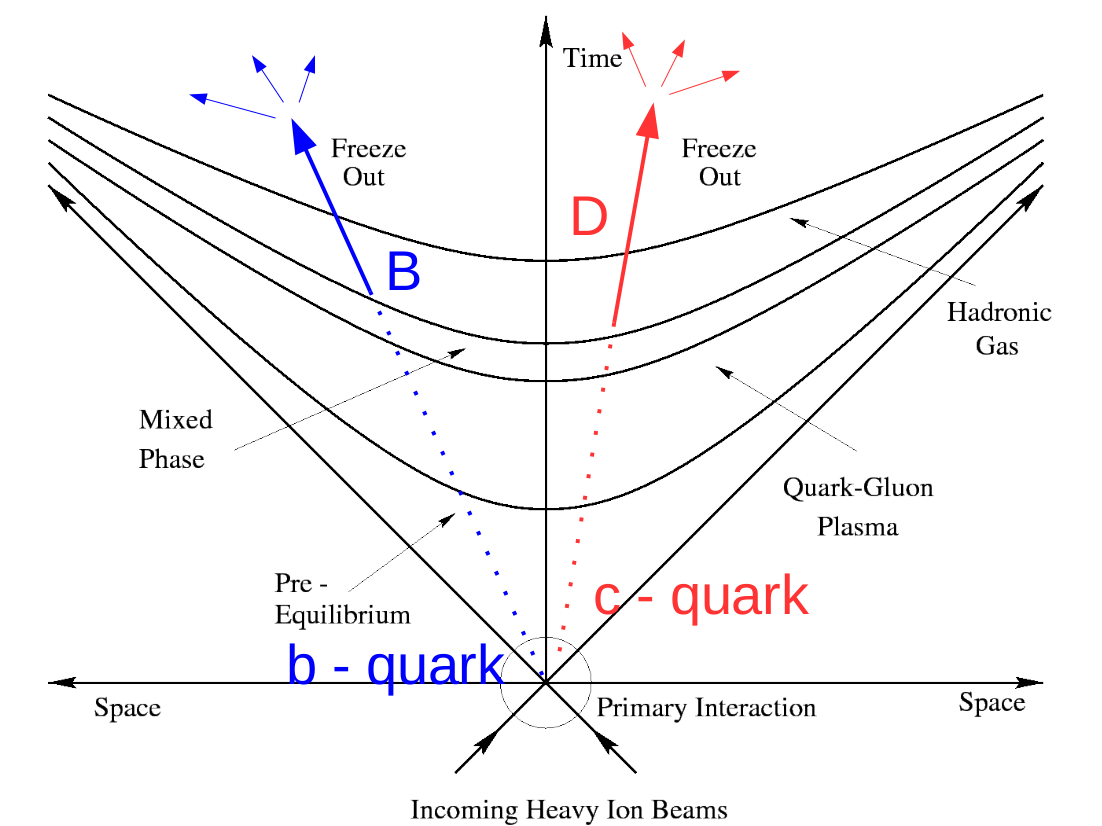
\includegraphics[scale=0.21]{st_cone_hf.png}}

\put(185,245){\captionsetup{labelformat=empty}
\begin{minipage}[t]{0.44\linewidth}
\begin{block}{}
\begin{center}
Gli \textit{heavy flavours} (quark $c$ e $b$) a causa dell'elevata massa 
\[m_c \simeq 1.5 \text{ GeV/c}^2, \text{ } m_b \simeq 4.5 \text{ GeV/c}^2\]
vengono prodotti nella fase iniziale della collisione (\textit{fase di pre-equilibrio}) 
\[\tau_{prod} \sim \frac{\hslash}{m_{b,c}} \sim 0.05-0.1 \text{ fm/c} \]
\end{center}
\end{block}
\end{minipage}}

\put(-5,90){\captionsetup{labelformat=empty}
\begin{minipage}[t]{0.55\linewidth}
\begin{center}
Se nella collisione si crea un mezzo deconfinato (\textit{Quark-Gluon Plasma}), gli heavy flavours interagiscono con esso perdendo energia a causa di scattering elastici con i partoni del mezzo stesso e per radiazione di gluoni (\textit{gluonsstrahlung})
\[\langle \Delta E \rangle \propto \alpha_s C_R \hat{q}L^2\]
\end{center}
\end{minipage}}

\put(230,75){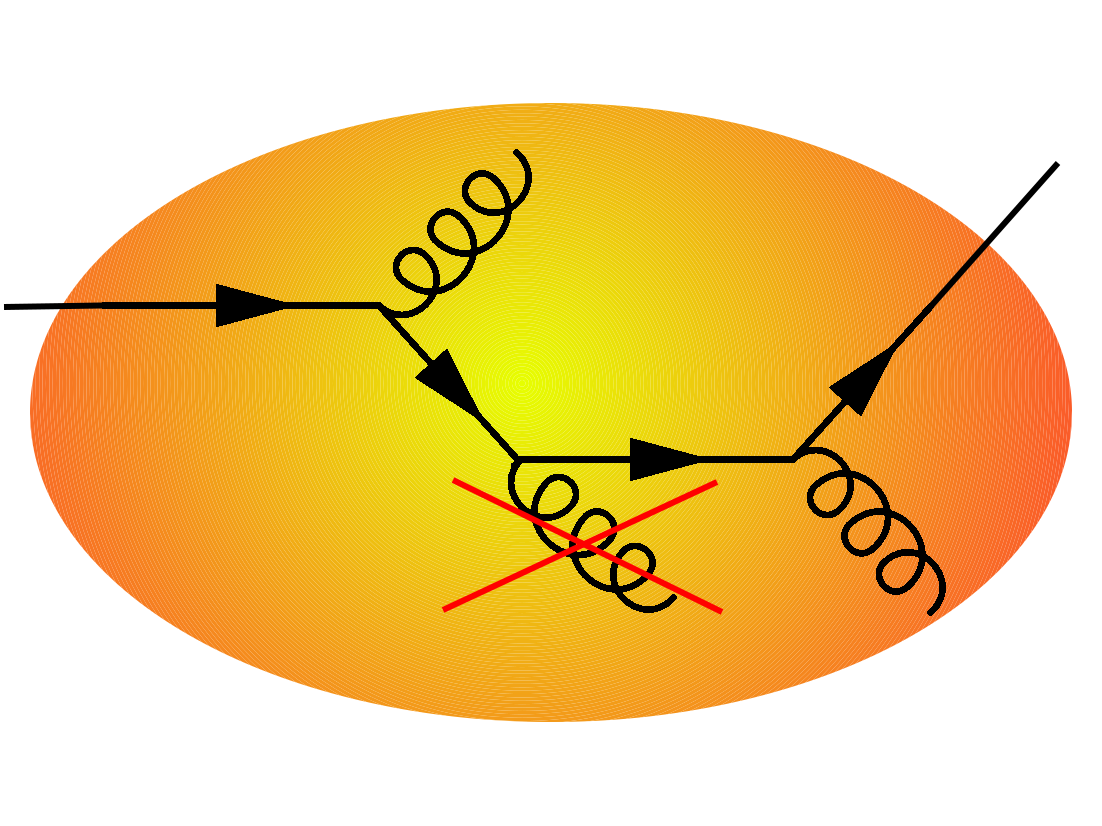
\includegraphics[scale=0.065]{energy_loss.png}}

\put(200,70){\captionsetup{labelformat=empty}
\begin{minipage}[t]{0.4\linewidth}
\begin{center}
La radiazione di gluoni dipende dalla massa del quark, in particolare risulta soppressa per 
\[\theta < \frac{M_q}{E_g} \hspace{2cm}\] 
\end{center}
\end{minipage}}

\put(270,30){\captionsetup{labelformat=empty}
\begin{minipage}[t]{0.4\linewidth}
\textcolor{blue}{DEAD CONE \\EFFECT}
\end{minipage}}

\end{picture} 
\end{frame}

\begin{frame}
\frametitle{\textit{Open heavy flavours} in collisioni p-Pb}
\begin{picture}(320,250)

\put(-5,15){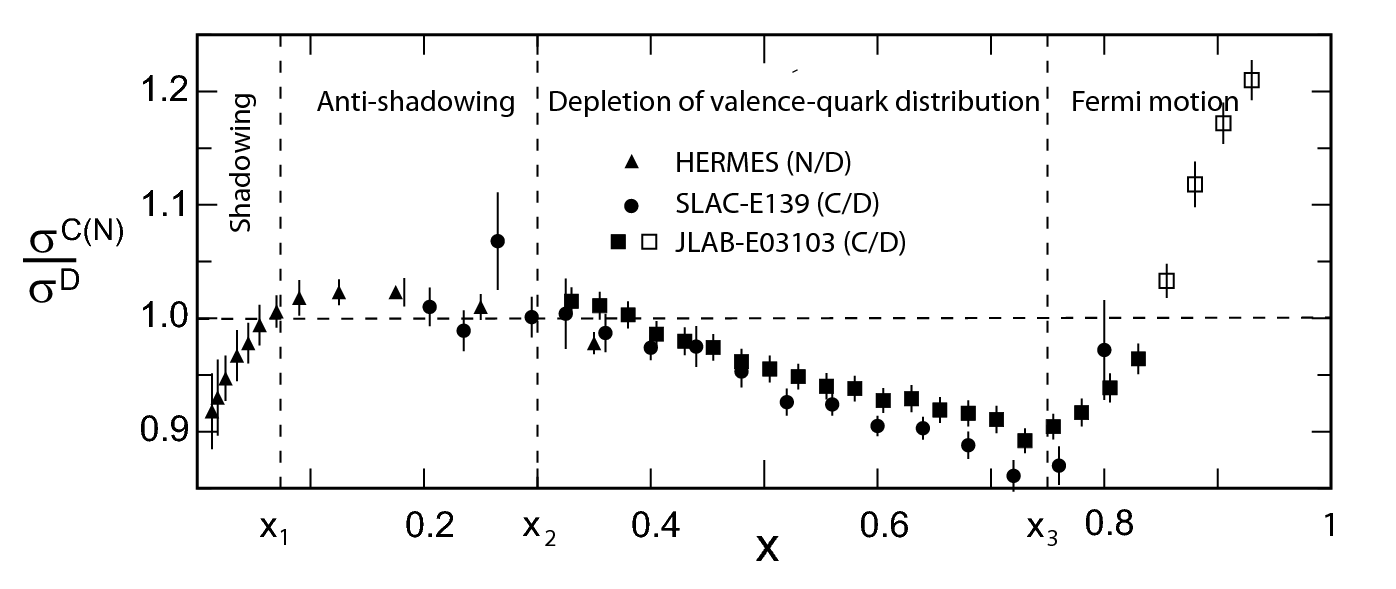
\includegraphics[scale=0.12]{PDF_nuclear_2}}
\put(230,100){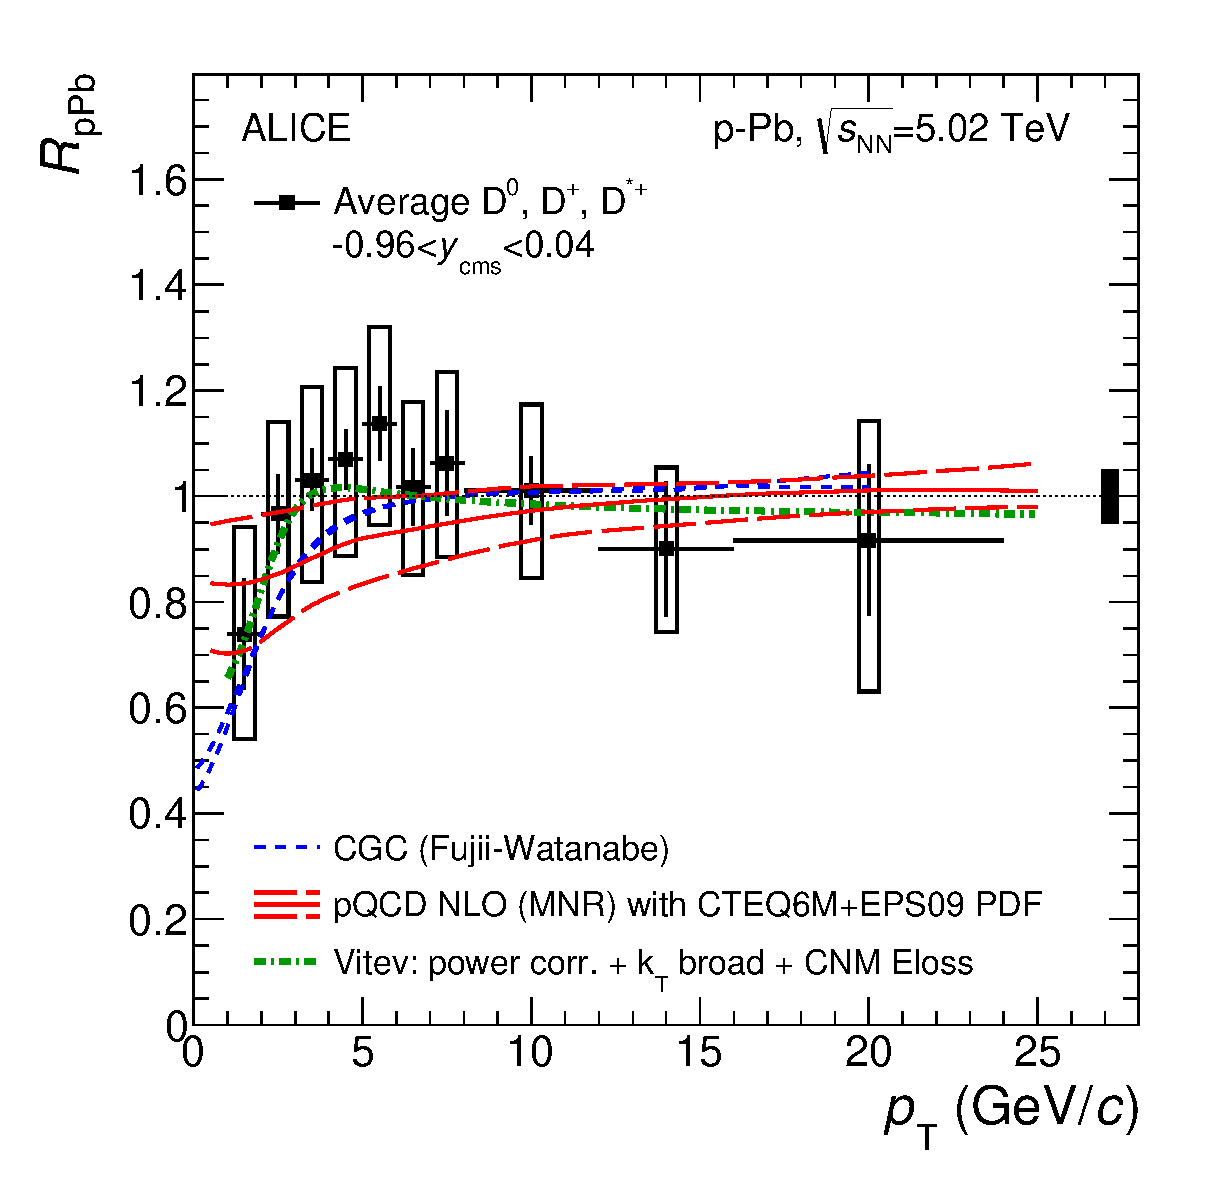
\includegraphics[scale=0.21]{pPbWithModels.eps}}

\put(0,235){\captionsetup{labelformat=empty}
\begin{minipage}[t]{1.\linewidth}
\begin{center}
 Nelle collisioni p-Pb non si raggiungono le condizioni per la formazione di un QGP esteso
 $\Rightarrow$ ci permettono di studiare i \textit{Cold Nuclear Matter Effects}
 \begin{itemize}
 \color{blue}
  \item Cronin Enhancement
  \vspace{3.5cm}
  \item Modifica delle PDF in presenza di materia nucleare
 \end{itemize}
\end{center}
\end{minipage}}

\put(10,197){\captionsetup{labelformat=empty}
\begin{minipage}[t]{0.6\linewidth}
Le collisioni multiple dei partoni del proiettile con i nucleoni del nucleo determinano uno \textit{shift} dello spettro a più alti valori di $\pt$
\end{minipage}}

\put(55,170){\captionsetup{labelformat=empty}
\begin{minipage}[t]{0.35\linewidth}
\begin{block}{Nuclear modification factor}
\setlength\abovedisplayskip{-1pt}
\[R_{pPb} (\pt) = \frac{1}{<N_{coll}>}\frac{dN_{pPb}/d\pt}{dN_{pp}/d\pt}\]
\end{block}
\end{minipage}}

\put(170,80){\captionsetup{labelformat=empty}
\begin{minipage}[t]{0.58\linewidth}
Si possono distringuere quattro regioni:
\begin{itemize}
 \item $x \lesssim 0.1$ $\rightarrow$ \textit{shadowing region} 
 \item $0.1 \lesssim x \lesssim 0.2$ $\rightarrow$ \textit{anti-shadowing region} 
 \item $0.2 \lesssim x \lesssim 0.8$ $\rightarrow$ \textit{EMC effect} 
 \item $x \gtrsim 0.8$ $\rightarrow$ moto di Fermi
\end{itemize}
\end{minipage}}

\end{picture} 
\end{frame}

\section{ALICE}
\begin{frame}
\frametitle{A Large Ion Collider Experiment}
\begin{picture}(320,250)

\put(0,80){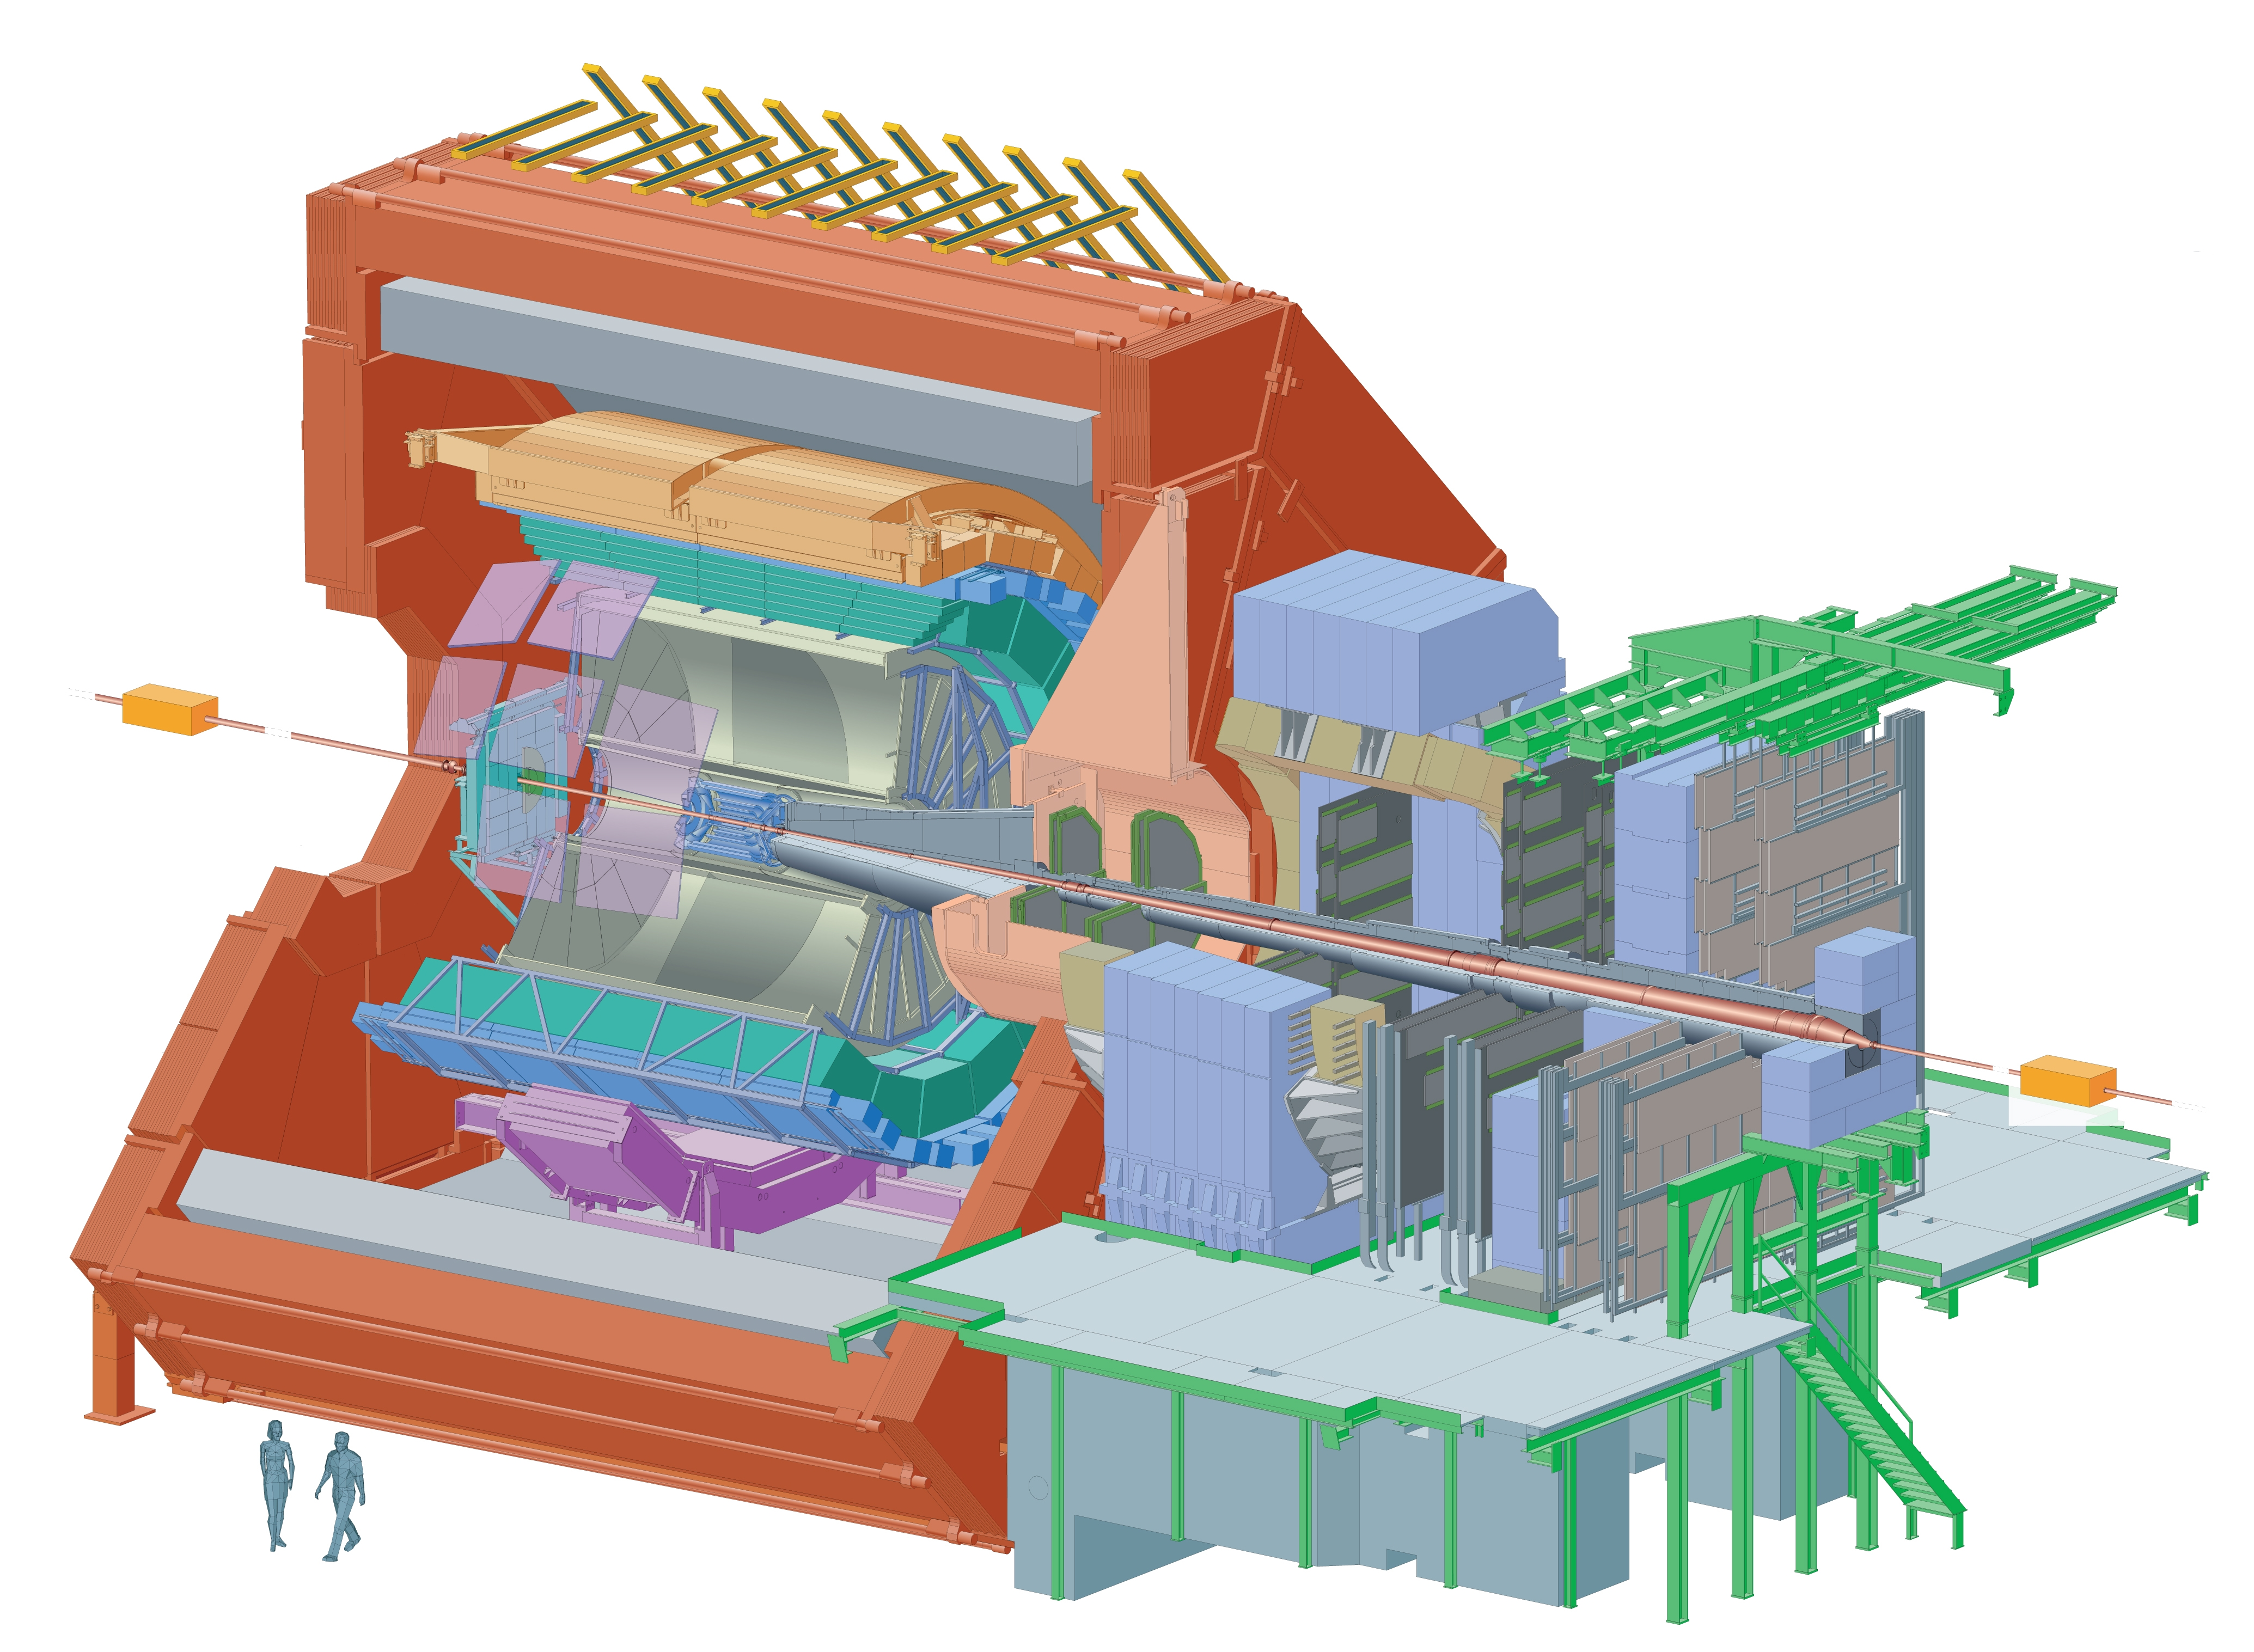
\includegraphics[scale=0.055]{2012-Aug-02-ALICE_3D_v0.jpg}}
\put(10,10){\fcolorbox{red}{white}{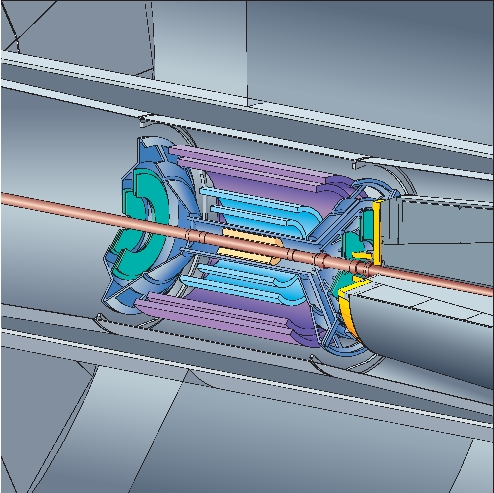
\includegraphics[scale=0.18]{2012-Aug-02-ALICE_3D_ITS}}}
\put(225,160){\fcolorbox{verdebbello}{white}{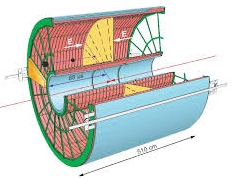
\includegraphics[scale=0.5]{TPC.jpeg}}}
\put(235,20){\fcolorbox{blue}{white}{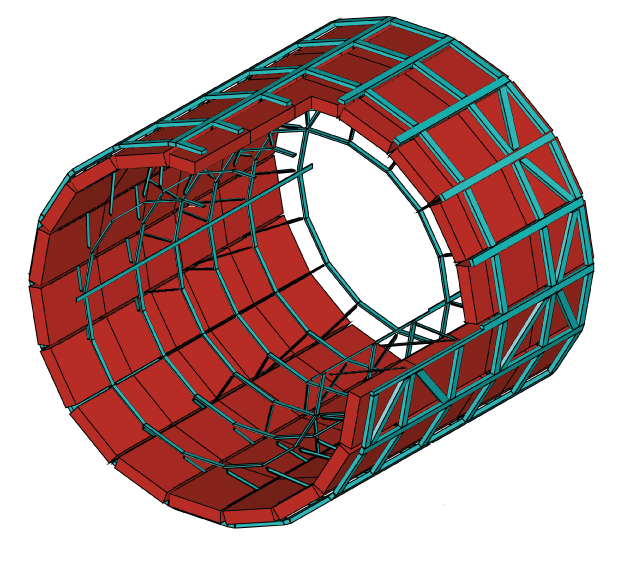
\includegraphics[scale=0.13]{TOF.png}}}

\put(50,80){
\begin{tikzpicture}[->]
\draw[draw=red,solid,line width=0.3mm] (0, 0) -- + (-0.75,-2.8);
\end{tikzpicture}}

\put(95,175){
\begin{tikzpicture}[->]
\draw[draw=verdebbello,solid,line width=0.3mm] (0, 0) -- + (4.3,1);
\end{tikzpicture}}

\put(95,80){
\begin{tikzpicture}[->]
\draw[draw=blue,solid,line width=0.3mm] (0, 0) -- + (4.5,-1.8);
\end{tikzpicture}}

\put(80,60){\captionsetup{labelformat=empty}
\begin{minipage}[t]{0.53\linewidth}
 \hspace{0.1cm} \fcolorbox{red}{white}{{Inner Tracking System}}
\small
\begin{itemize}
\item 2 layer Silicon Pixel Detector
 \item 2 layer Silicon Drift Detector
 \item 2 layer Silicon Strip Detector
\end{itemize}
\end{minipage}}

\put(241,105){\captionsetup{labelformat=empty}
\begin{minipage}[t]{0.53\linewidth}
 \hspace{0.1cm} \fcolorbox{blue}{white}{{Time of Flight}}
\end{minipage}}

\put(230,145){\captionsetup{labelformat=empty}
\begin{minipage}[t]{0.53\linewidth}
 \hspace{0.1cm} \fcolorbox{verdebbello}{white}{{Time Projection Chamber}}
\end{minipage}}

\end{picture} 
\end{frame}

\section{Ricostruzione di mesoni D$^+$}
\begin{frame}
\frametitle{Ricostruzione e selezione di mesoni D$^+$ in ALICE}
\begin{picture}(320,250)

\put(210,90){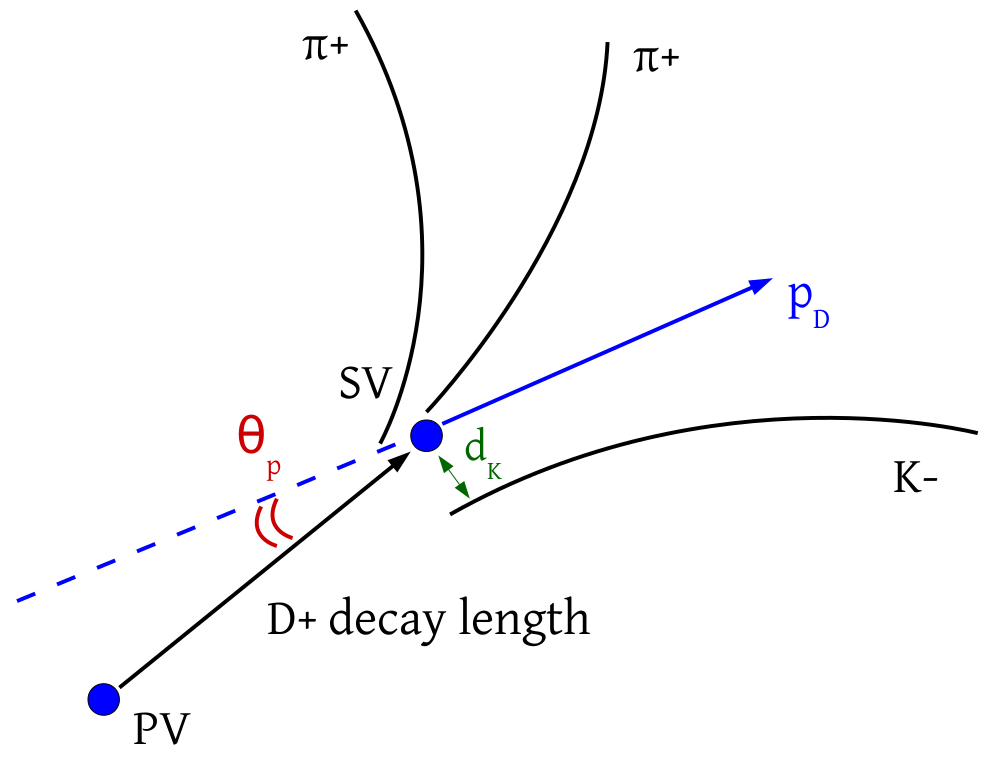
\includegraphics[scale=0.18]{Dplus_sketch.png}}
\put(5,20){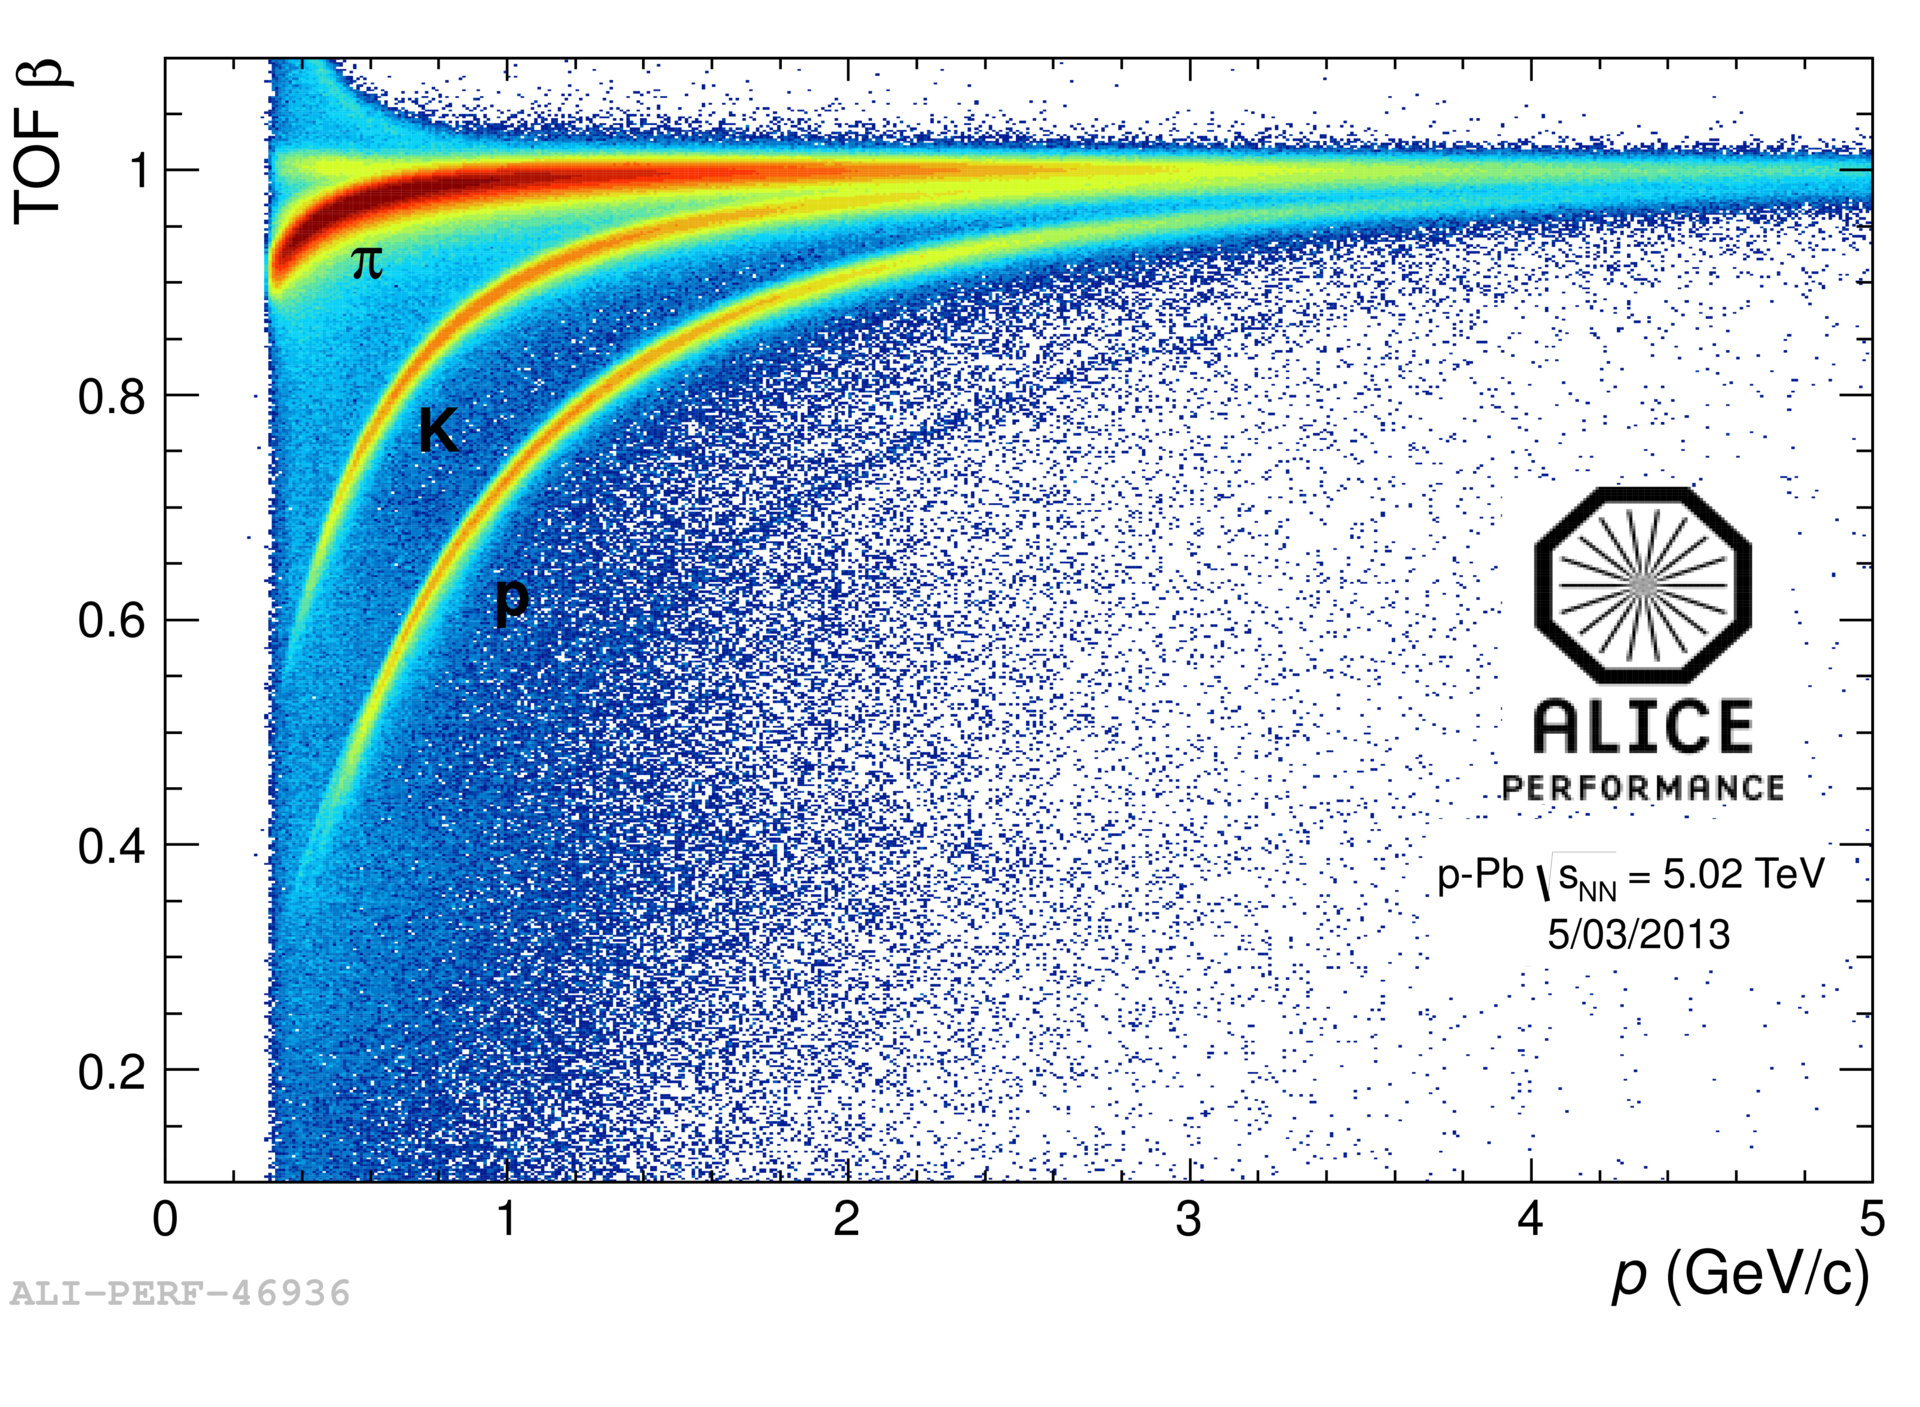
\includegraphics[scale=0.08]{2013-Mar-06-betap_v5.png}}

\put(0,230){\captionsetup{labelformat=empty}
\begin{minipage}[t]{1.\linewidth}
Mesoni D$^+$ ($c\tau = 312\text{ } \mu$m) ricostruiti nel canale di decadimento adronico
\end{minipage}}

\put(105,230){\captionsetup{labelformat=empty}
\begin{minipage}[t]{0.35\linewidth}
\begin{block}{}
 \setlength\abovedisplayskip{-0.5pt}
\[\text{D}^+\rightarrow \text{K}^-\pi^+\pi^+ (BR = 9.13\%)\] 
\end{block}
\end{minipage}}

\put(0,190){\captionsetup{labelformat=empty}
\begin{minipage}[t]{1.\linewidth}
\begin{itemize}
 \item Il segnale è estratto con un'\textcolor{blue}{analisi di massa invariante}
 \vspace{0.2cm}
 \item Vengono applicate selezioni topologiche \\sulle quantità ricostruite per \\ridurre il fondo combinatoriale
\end{itemize}
\end{minipage}}

\put(160,70){\captionsetup{labelformat=empty}
\begin{minipage}[t]{0.53\linewidth}
\begin{itemize}
 \item Per rimuovere ulteriormente del fondo viene applicata la \textit{Particle Identification} (PID) nella selezione delle tracce nello stato finale 
\end{itemize}
\end{minipage}}

\end{picture} 
\end{frame}

\section{Metodi theory-driven per la misura della frazione di D$^+$ prompt}
\begin{frame}
\frametitle{Mesoni D$^+$ primari e secondari}
\begin{picture}(320,250)

\put(10,25){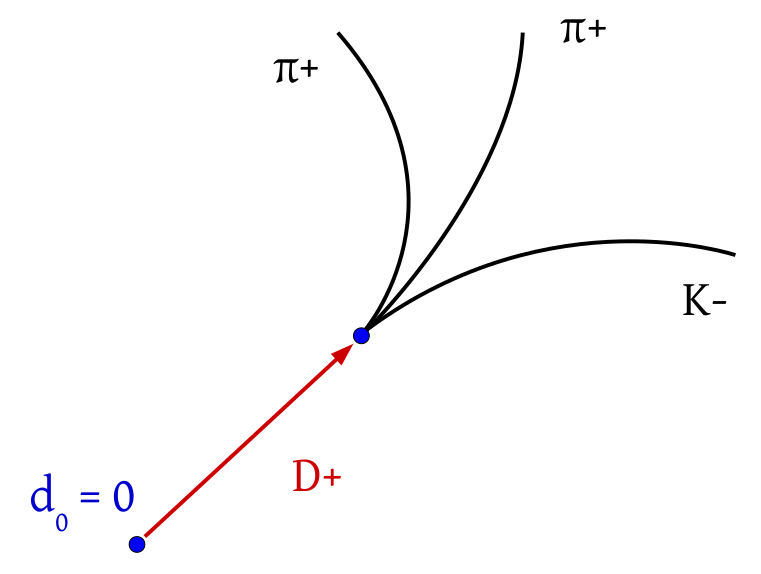
\includegraphics[scale=0.25]{Prompt_sketch.png}}
\put(180,20){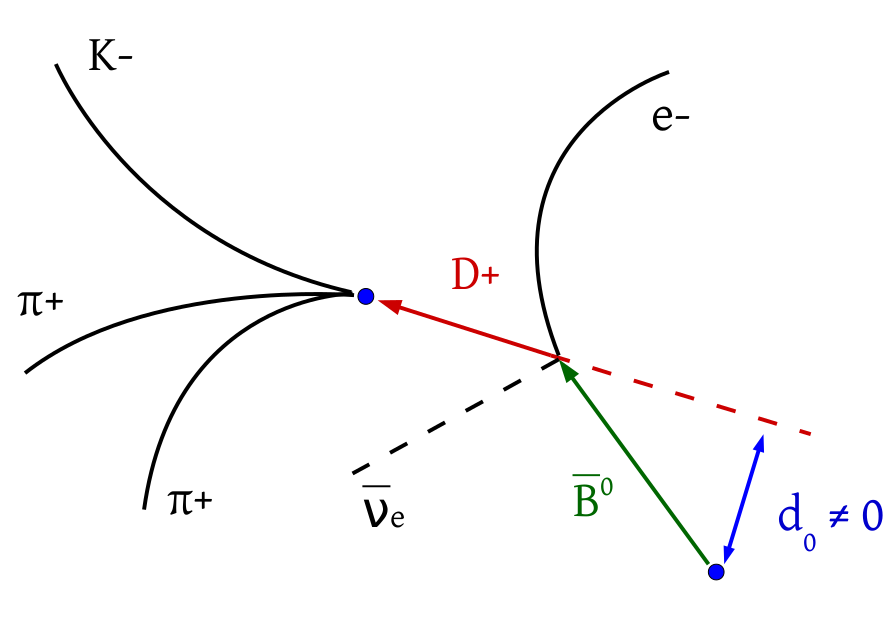
\includegraphics[scale=0.25]{FD_sketch.png}}

\put(10,230){\captionsetup{labelformat=empty}
\begin{minipage}[t]{1.1\linewidth}
Per la misura dei mesoni D$^+$ che sono originati da un quark \textit{charm} prodotto nella \\collisione è necessario separare il contributo di D$^+$ prompt dal segnale totale
\end{minipage}}

\put(15,205){\captionsetup{labelformat=empty}
\begin{minipage}[t]{0.4\linewidth}
\begin{block}{\centering D$^+$ primari (\textit{prompt})}
\begin{center}
 Derivano direttamente dall'adronizzazione di un quark $c$ \\
 $c \rightarrow \text{D}^+$
\end{center}
\end{block}
\end{minipage}}

\put(190,205){\captionsetup{labelformat=empty}
\begin{minipage}[t]{0.4\linewidth}
\begin{block}{\centering D$^+$ secondari (\textit{feed-down})}
\begin{center}
 Derivano dal decadimento di un mesone B \\
 $b \rightarrow \text{B} \rightarrow \text{D}^++\text{X}$
\end{center} 
\end{block}
\end{minipage}}

\end{picture} 
\end{frame}

\begin{frame}
\frametitle{Metodi \textit{theory-driven} per la misura della frazione di mesoni D$^+$ prompt}
\begin{picture}(320,250)

\put(180,15){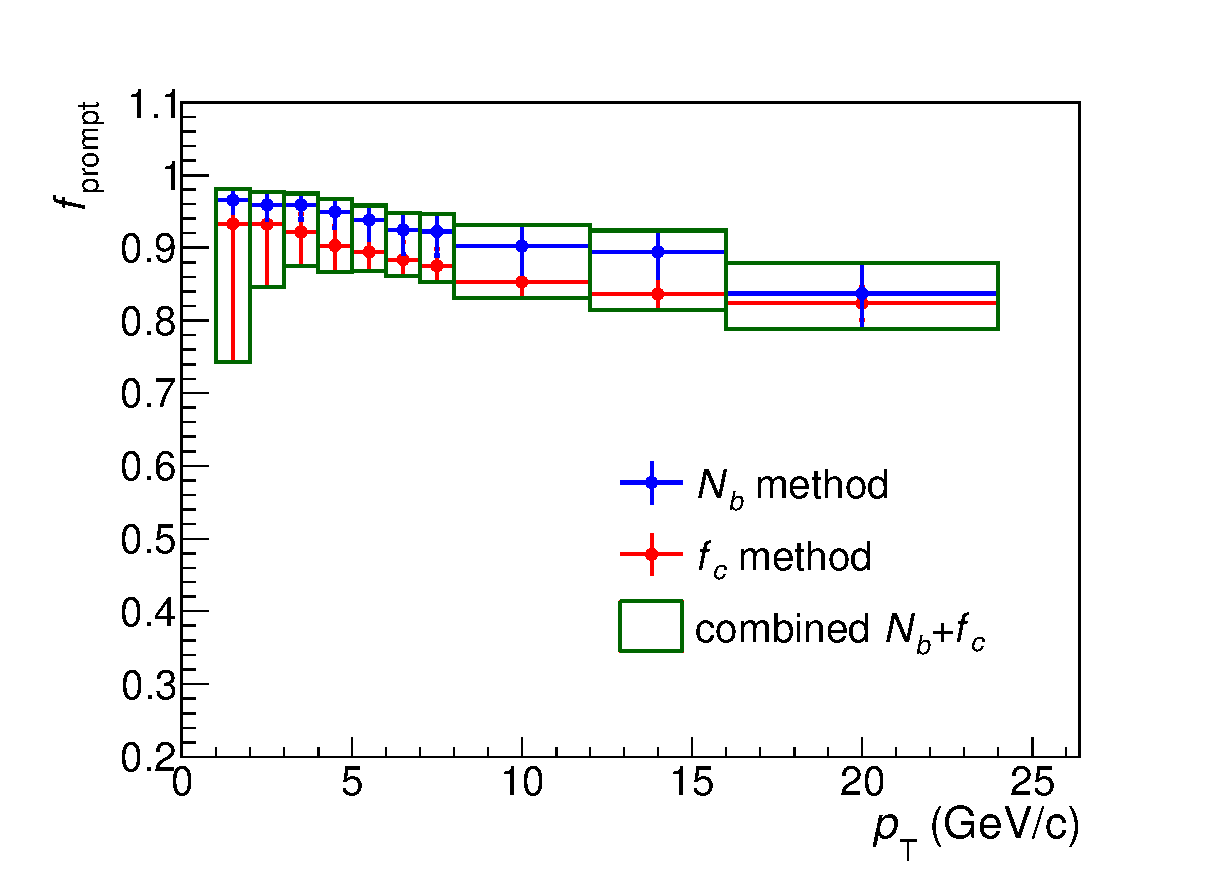
\includegraphics[scale=0.3]{Fprompt_fc_Nb_comp.eps}}

\put(0,235){\captionsetup{labelformat=empty}
\begin{minipage}[t]{1.\linewidth}
La frazione di D$^+$ prompt può essere ottenuta utilizzando metodi \textit{theory-driven}
\end{minipage}}

\put(0,230){\captionsetup{labelformat=empty}
\begin{minipage}[t]{1.\linewidth}
\vspace{0.2cm}
\begin{itemize}
\item Metodo $N_b$ 
 \vspace{-0.2cm}
 \[f_{prompt} = 1-A\cdot \textcolor{blue}{\bigg{(}\frac{d^2\sigma}{d\pt dy}\bigg{)}_{FONLL}^{feed-down}R_{pPb}^{feed-down}(\pt)}\frac{(Acc\times \epsilon)_{feed-down}\cdot\Delta y \Delta\pt \cdot BR \cdot L_{int}}{N_{raw}^{D^\pm}/2}\]
  \item Metodo $f_c$
 \vspace{-0.5cm}
 \[f_{prompt} = \bigg{(} 1+\frac{\textcolor{blue}{\frac{d^2\sigma}{d\pt dy}_{FONLL}^{feed-down}}\cdot(Acc\times \epsilon)_{feed-down}\cdot\textcolor{blue}{R_{pPb}^{feed-down}(\pt)}}{\textcolor{blue}{\frac{d^2\sigma}{d\pt dy}_{FONLL}^{prompt}}\cdot(Acc\times \epsilon)_{prompt}\cdot R_{pB}^{prompt}(\pt)}\bigg{)}^{-1}\]
\end{itemize}
\end{minipage}}

\put(0,100){\captionsetup{labelformat=empty}
\begin{minipage}[t]{0.95\linewidth}
Principali sorgenti di errore sistematico:
\begin{itemize}
 \item Calcolo perturbativo di \textcolor{blue}{$\bigg{(}\frac{d^2\sigma}{d\pt dy}\bigg{)}_{FONLL}$}
 \item \textcolor{blue}{$R_{pPb}^{feed-down}(\pt)$} mai misurato \\[2mm]$\Rightarrow$ necessità di un'assunzione 
\end{itemize}
\end{minipage}}

\end{picture} 
\end{frame}

\section{Sommario}
\begin{frame}
\frametitle{Sommario}
\begin{picture}(320,250)

\end{picture} 
\end{frame}

\section{Metodo di fit del parametro di impatto}
\begin{frame}
\frametitle{Metodo di fit del parametro di impatto}
\begin{picture}(320,250)

\put(25,132){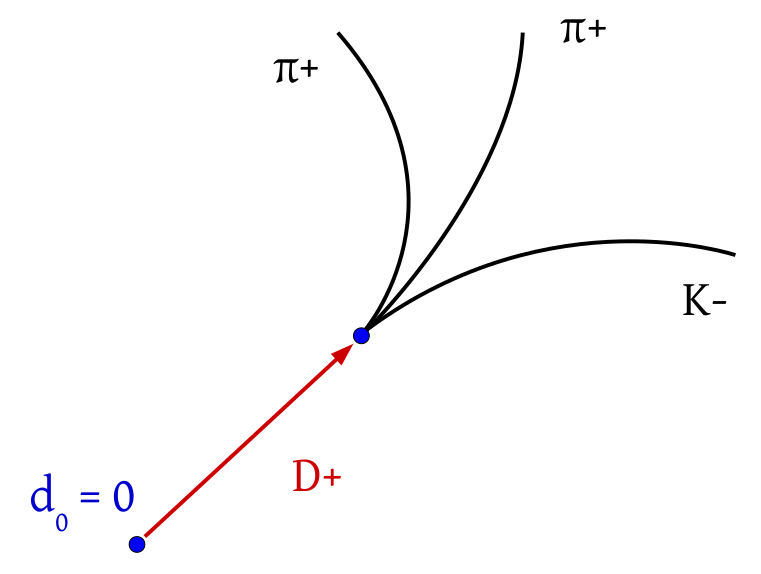
\includegraphics[scale=0.2]{Prompt_sketch.png}}
\put(180,130){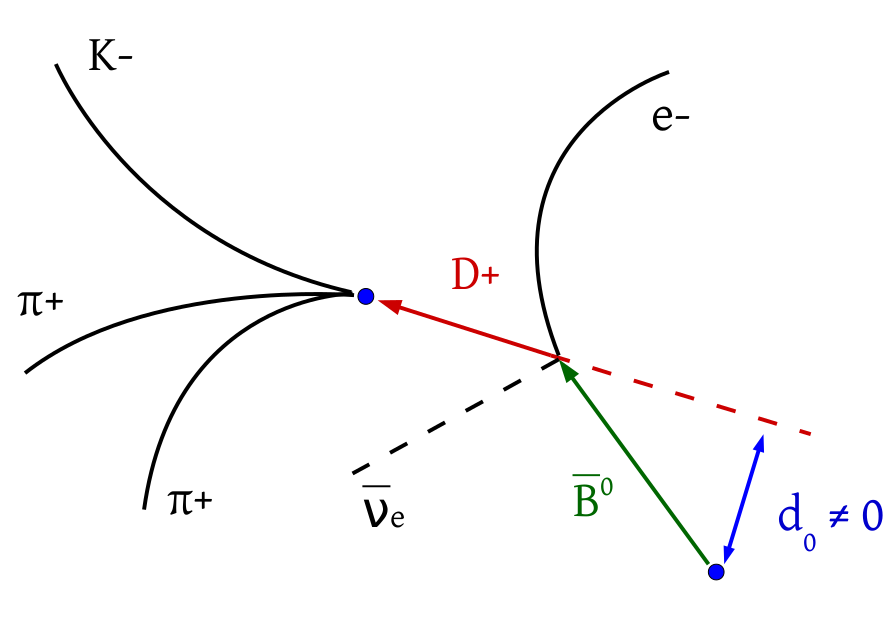
\includegraphics[scale=0.2]{FD_sketch.png}}

\put(0,235){\captionsetup{labelformat=empty}
\begin{minipage}[t]{0.95\linewidth}
Si basa sulla differenza tra le distribuzioni del parametro di impatto ($d_0$) di mesoni D$^+$ prompt e feed-down:
\end{minipage}}

\put(0,120){\captionsetup{labelformat=empty}
\begin{minipage}[t]{0.95\linewidth}
\begin{enumerate}
 \item \textcolor{blue}{Determinazione dei \textit{template} (fase di \textit{prefit})}
 \begin{itemize}
  \item Fit sulle distribuzioni simulate di mesoni D$^+$ prompt
  \item Fit sulle distribuzioni simulate di mesoni D$^+$ feed-down
  \item Fit sulle distribuzioni del fondo combinatoriale ottenute dai dati nelle regioni di massa invariante a lato del picco (\textit{side-bands})
 \end{itemize}
 \vspace{0.1cm}
  Nella fase di prefit si ottengono i parametri che vengono successivamente fissati nel fit finale dei dati per estrarre la frazione di mesoni D$^+$ prompt
 \vspace{0.2cm}
 \item \textcolor{blue}{Fit unbinned dei dati}\\
 La funzione di fit finale è somma dei singoli contributi
\end{enumerate}
\end{minipage}}

\end{picture} 
\end{frame}

\begin{frame}
\frametitle{Fit delle distribuzioni simulate di D$^+$ prompt e feed-down}
\begin{picture}(320,250)

\put(5,130){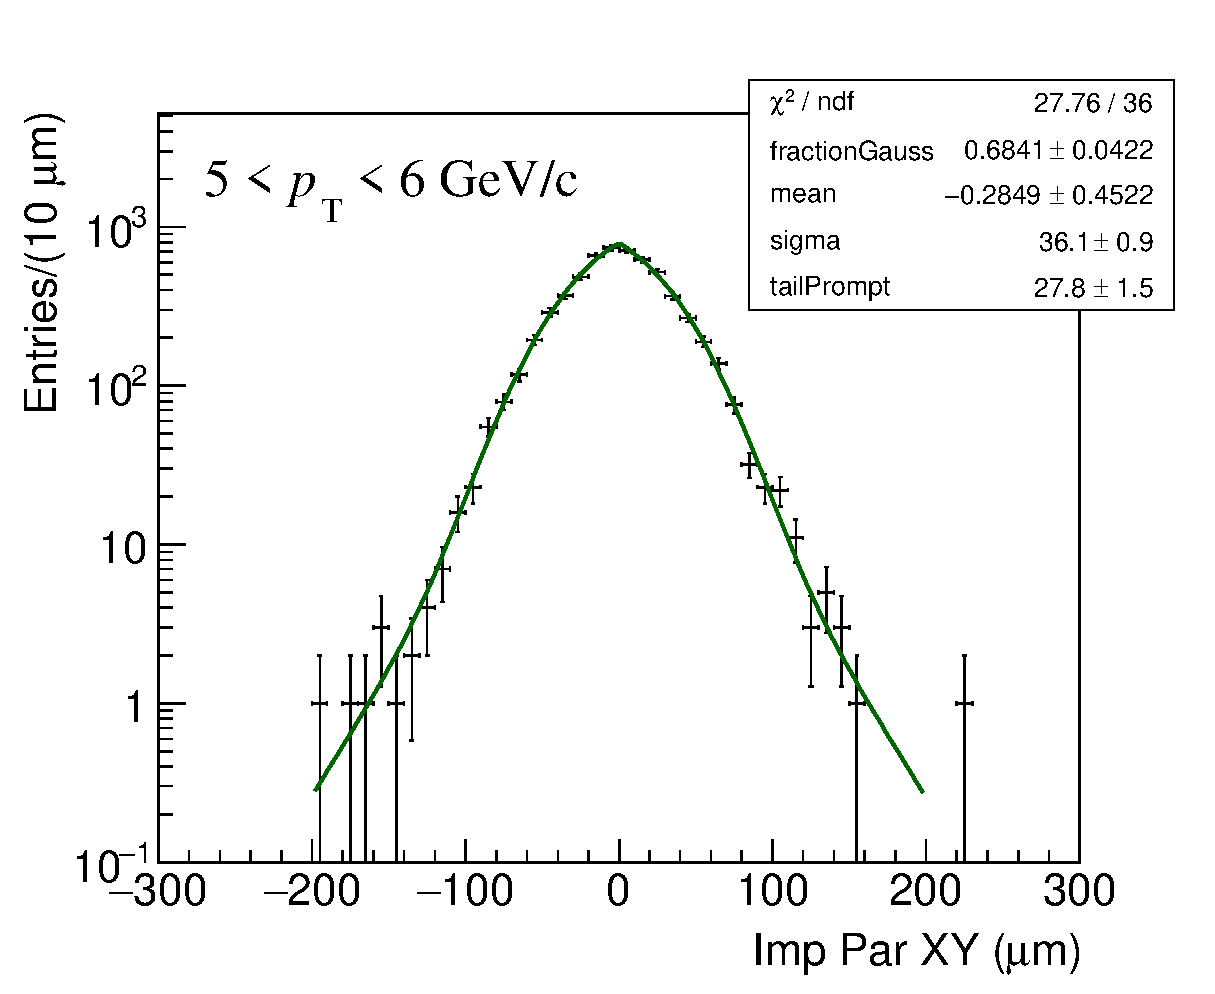
\includegraphics[scale=0.25]{ImpParPrompt_5-6.eps}}
\put(5,15){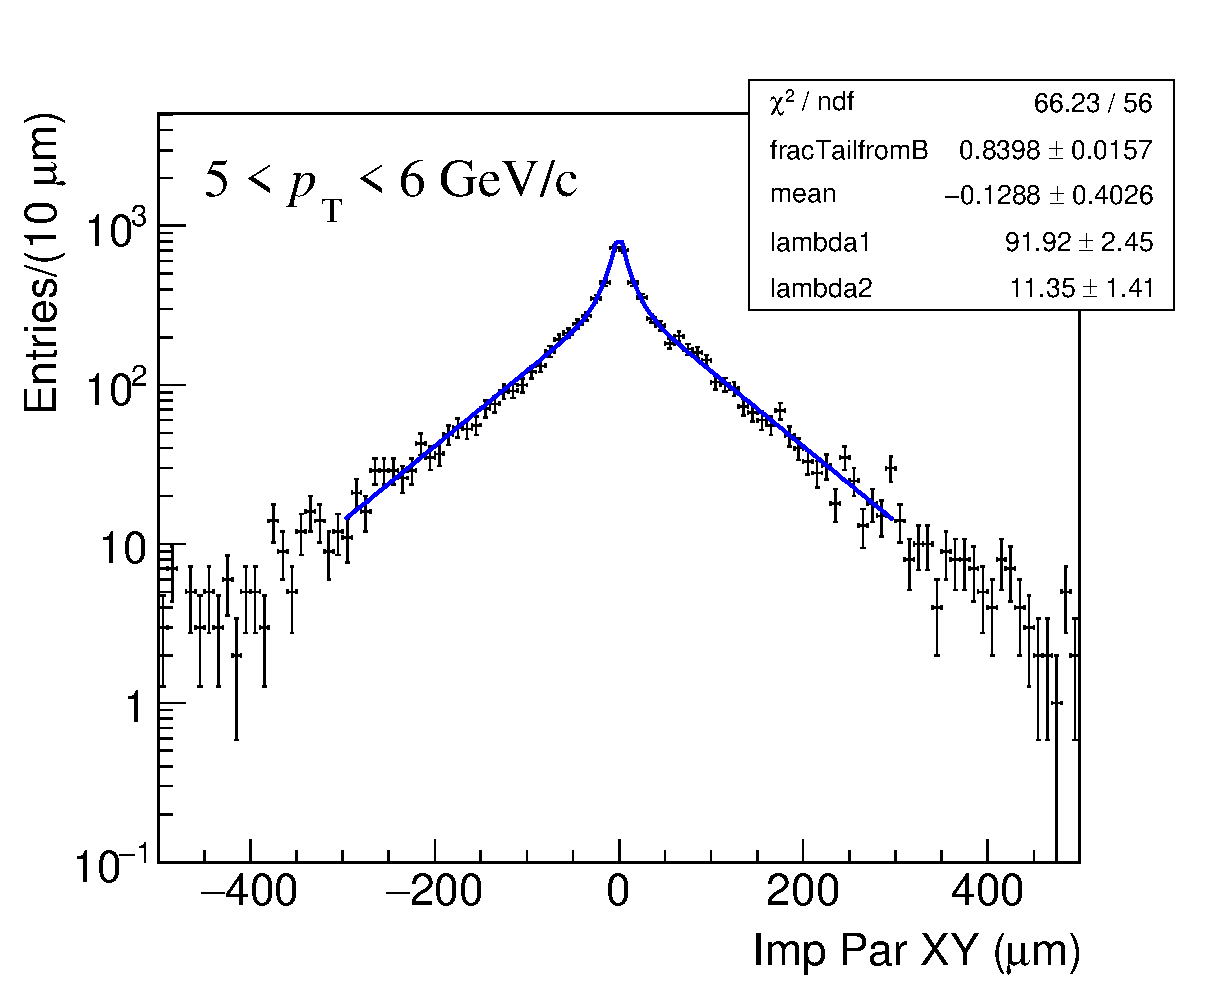
\includegraphics[scale=0.25]{ImpParTrueFD_5-6.eps}}
\put(210,15){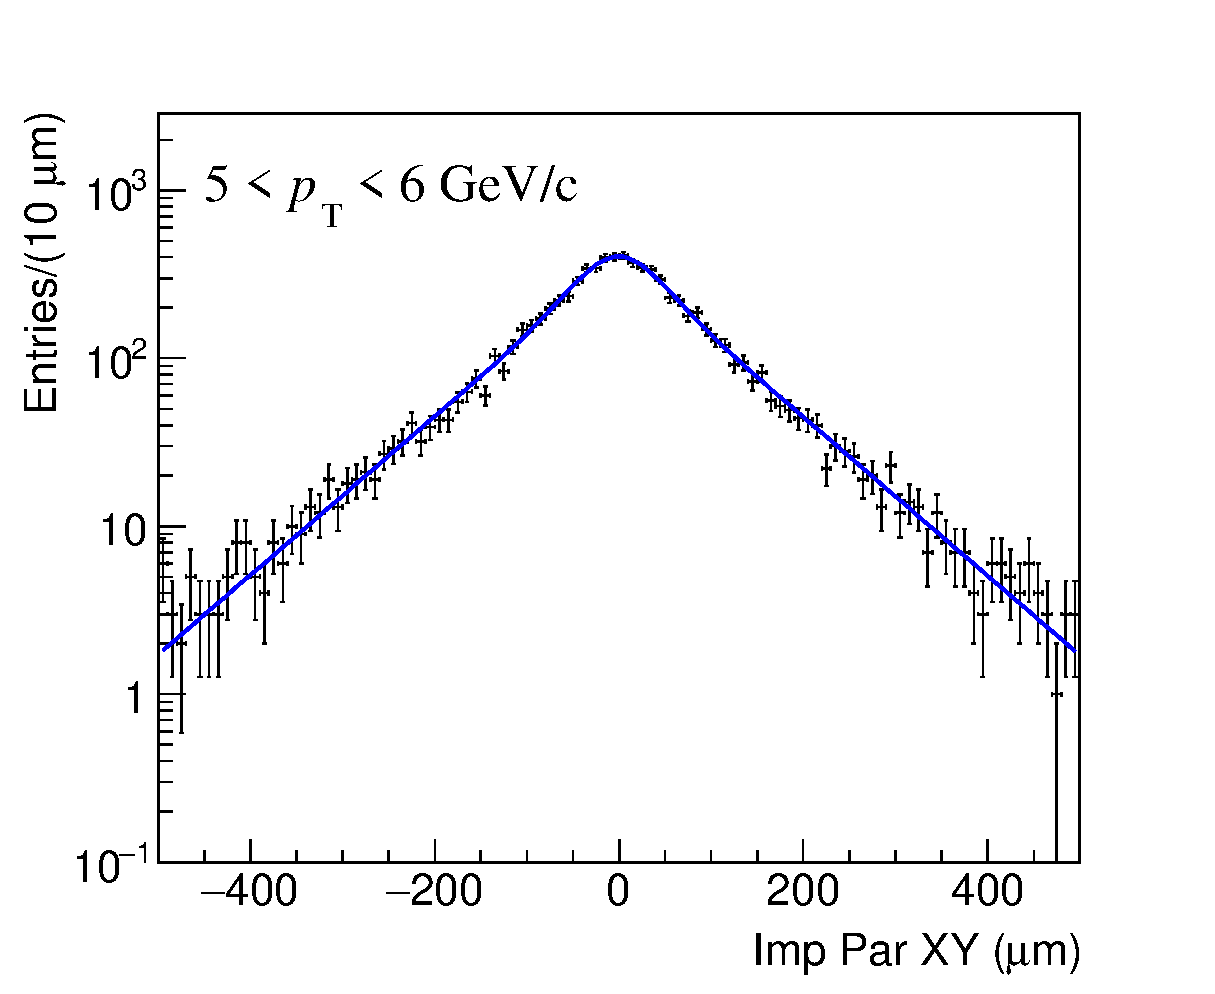
\includegraphics[scale=0.25]{ImpParRecoFD_5-6.eps}}

\put(160,230){\captionsetup{labelformat=empty}
\begin{minipage}[t]{0.5\linewidth}
\textcolor{verdebbello}{D$^+$ prompt}: fit della distribuzione del parametro di impatto \textit{simulato}\\
$\rightarrow$ somma di una Gaussiana e una funzione esponenziale simmetrica rispetto al valor medio
\end{minipage}}

\put(160,170){\captionsetup{labelformat=empty}
\begin{minipage}[t]{0.5\linewidth}
\textcolor{blue}{D$^+$ feed-down}: fit della distribuzione del parametro di impatto \textit{vero}\\
$\rightarrow$ somma di due funzioni esponenziali simmetriche rispetto al valor medio
\end{minipage}}

\put(145,85){
\begin{tikzpicture}[->]
\draw[draw=blue,solid,line width=0.3mm] (0, 0) -- + (1.8,0);
\end{tikzpicture}}

\put(145,65){\captionsetup{labelformat=empty}
\begin{minipage}[t]{0.2\linewidth}
Convoluzione\\[1mm] di \textcolor{blue}{$F^{feed-down}_{true}(d_0^{xy})$}\\[1mm] con \textcolor{verdebbello}{$F^{prompt}(d_0^{xy})$}
\end{minipage}}

\end{picture} 
\end{frame}

\begin{frame}
\frametitle{Fit delle distribuzioni del fondo combinatoriale}
\begin{picture}(320,250)

\put(5,130){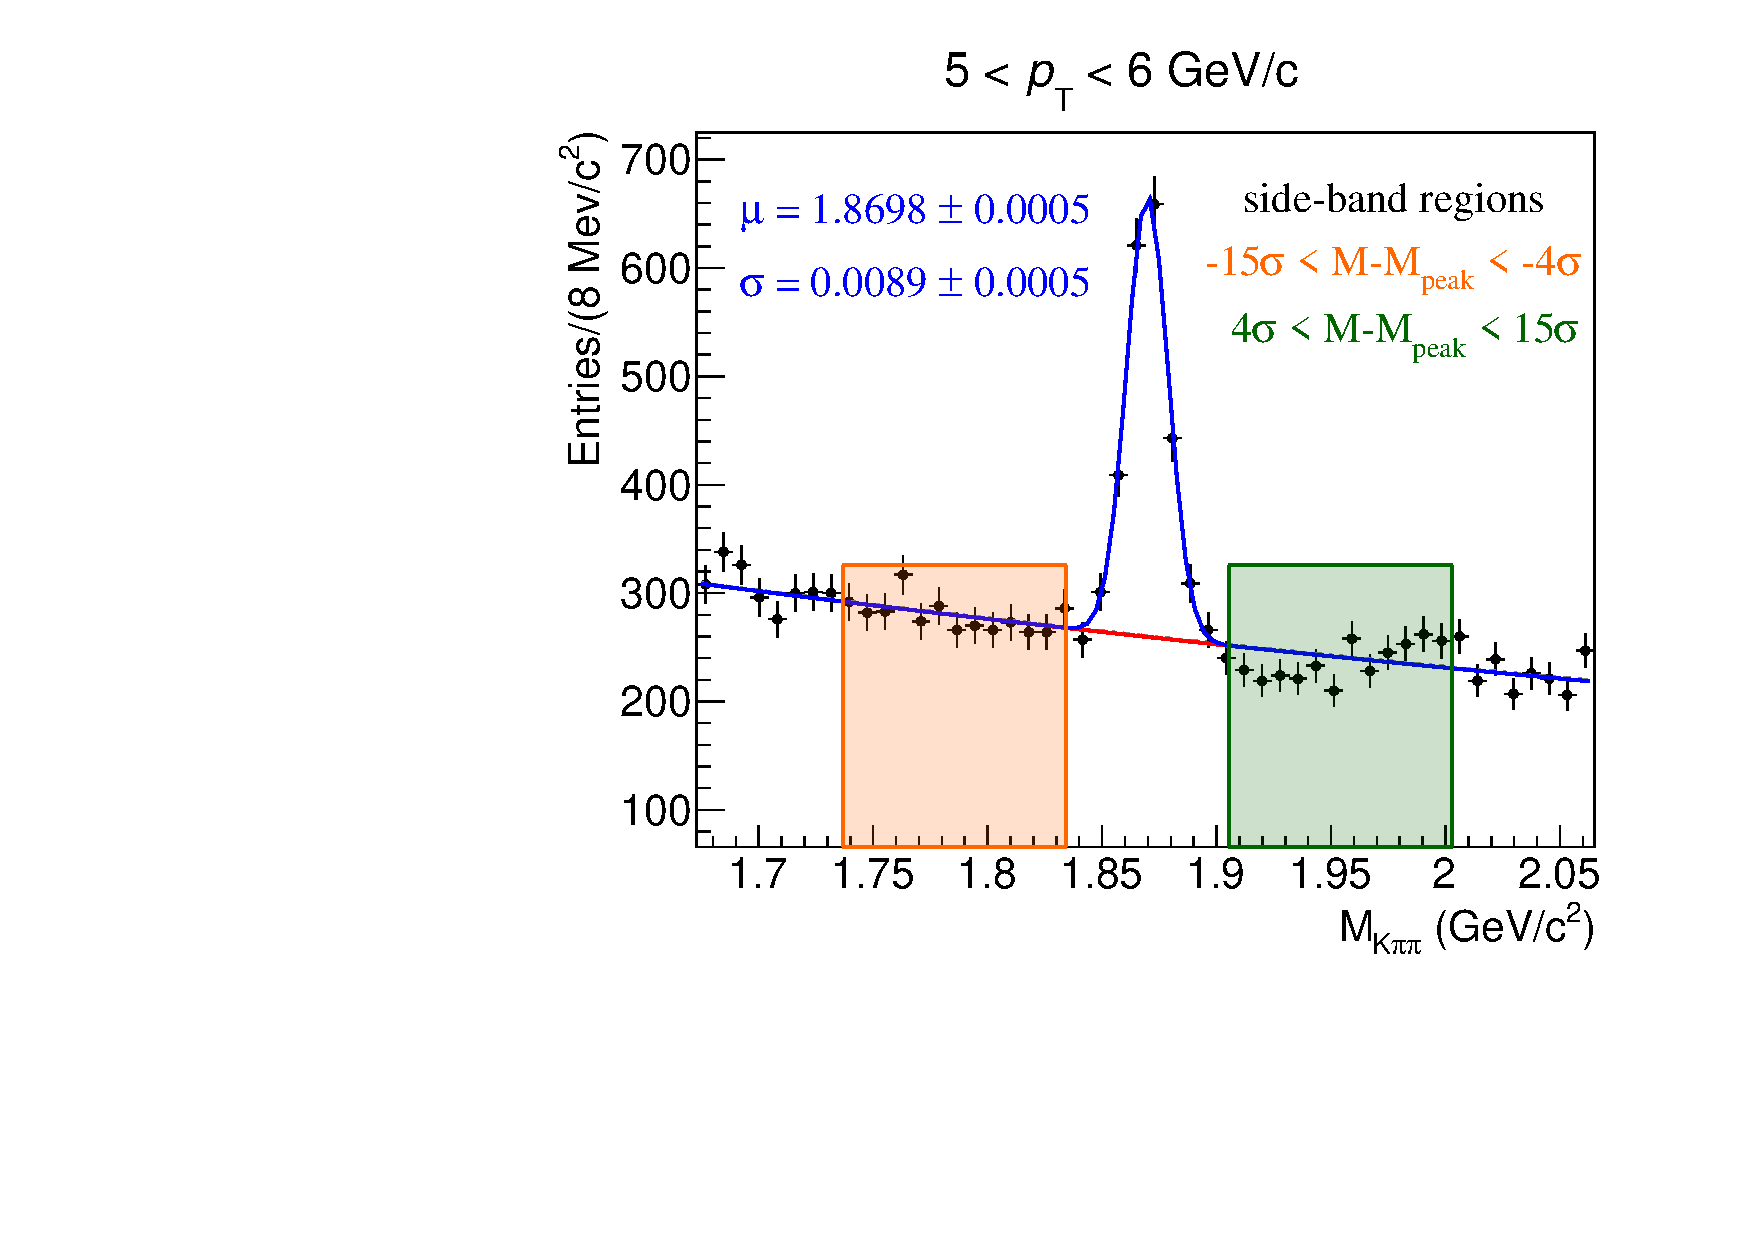
\includegraphics[scale=0.25]{Mass_5-6.pdf}}
\put(195,130){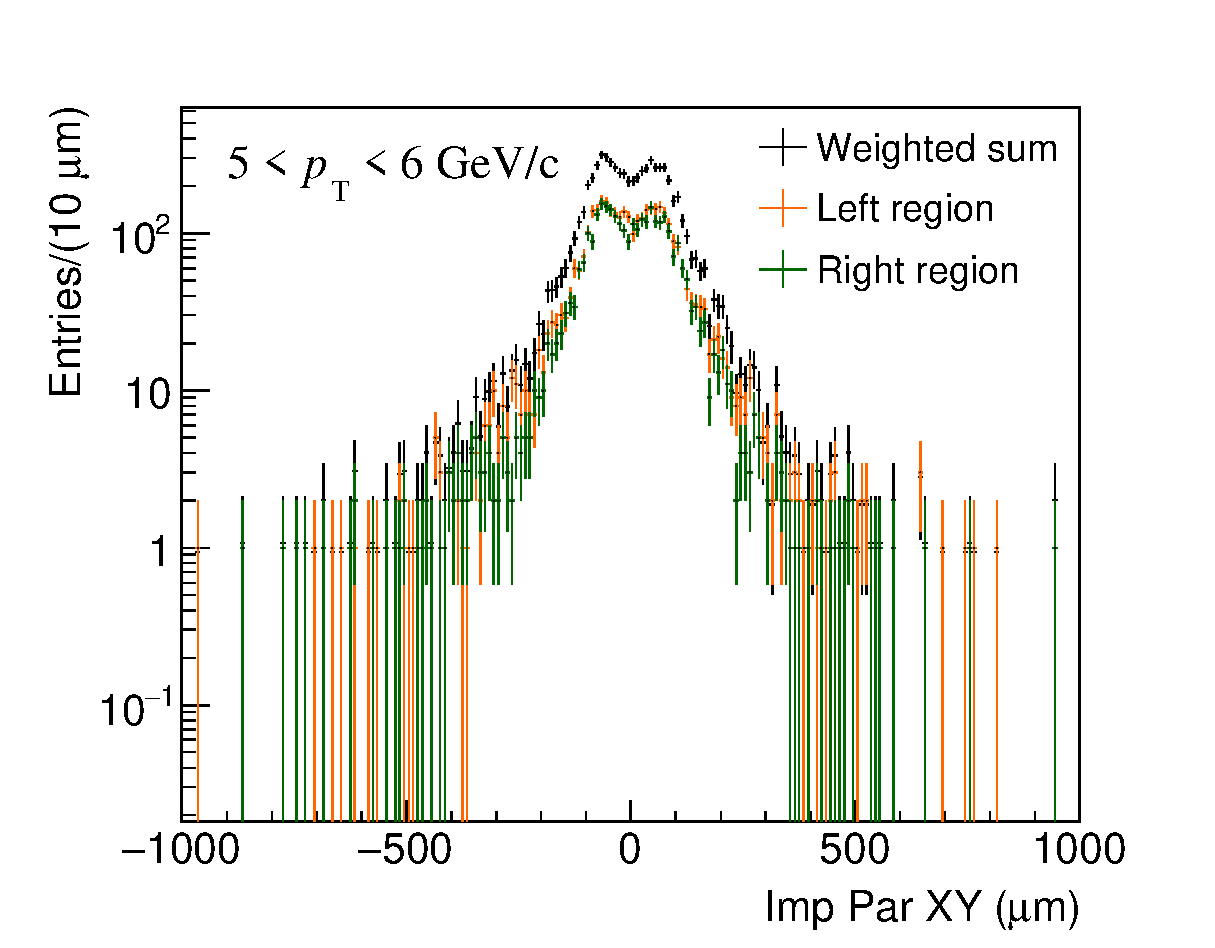
\includegraphics[scale=0.25]{Sidebands_Pt_5-6_NoFit.eps}}
\put(5,10){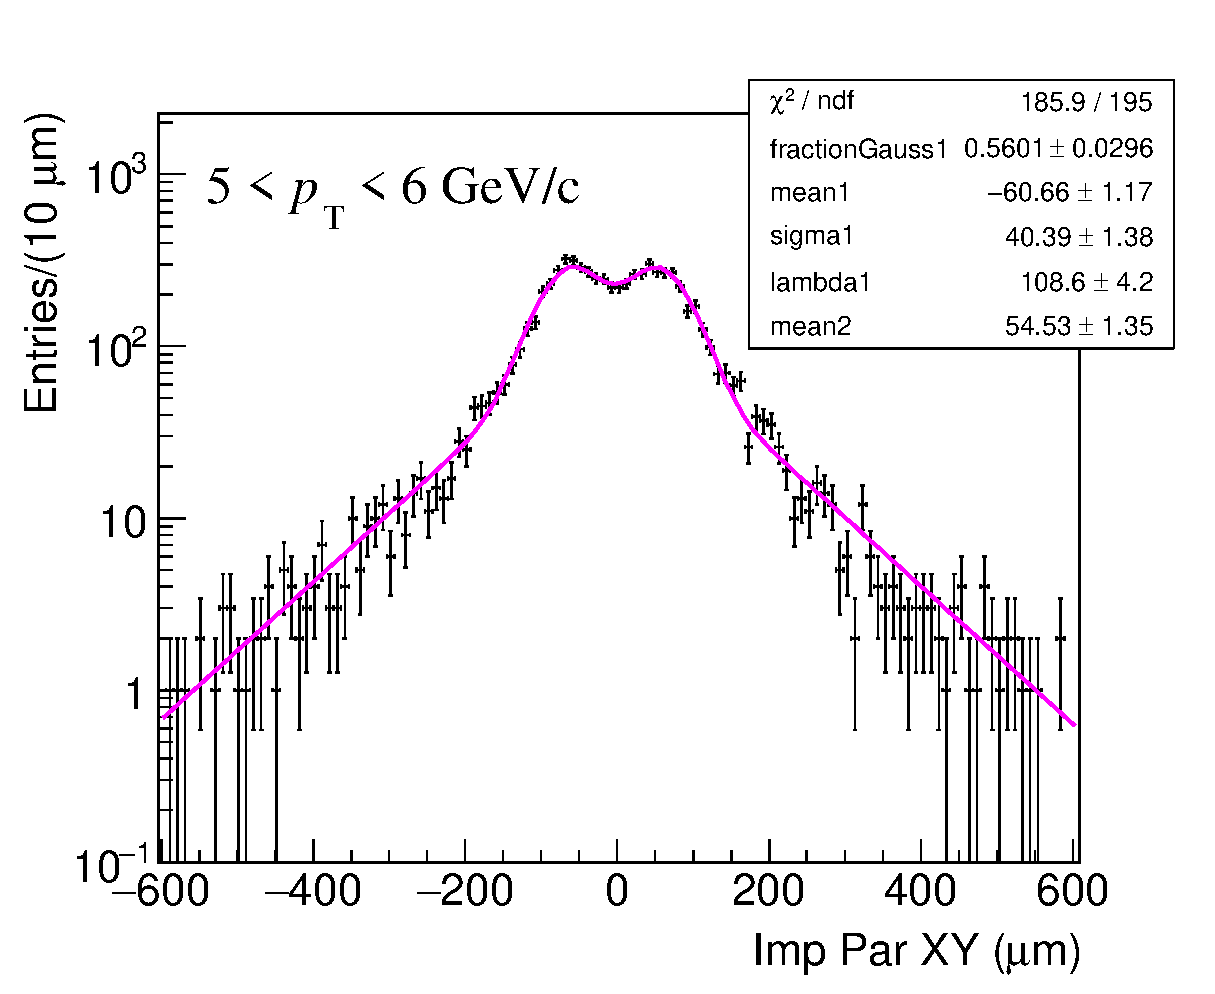
\includegraphics[scale=0.25]{ImpParBkg_5-6.eps}}

\put(113,150){
\begin{tikzpicture}[->]
\draw[draw=verdebbello,solid,line width=0.3mm] (0, 0) -- + (3.,0.5);
\end{tikzpicture}}

\put(66.5,170){
\begin{tikzpicture}[->]
\draw[draw=orange,solid,line width=0.3mm] (0, 0) -- + (4.6,0.5);
\end{tikzpicture}}

\put(160,100){\captionsetup{labelformat=empty}
\begin{minipage}[t]{0.5\linewidth}
\textcolor{magenta}{Fondo combinatoriale}: fit della distribuzione del parametro di impatto ottenuta dalle regioni di massa invariante a lato del picco (\textit{side-bands})
\[4\sigma<|M-M_{peak}|<15\sigma\]
$\rightarrow$ somma di due Gaussiane con code esponenziali, con i parametri uguali a meno dei valori medi
\end{minipage}}

\end{picture} 
\end{frame}

\begin{frame}
\frametitle{Fit \textit{unbinned} dei dati}
\begin{picture}(320,250)

\put(5,135){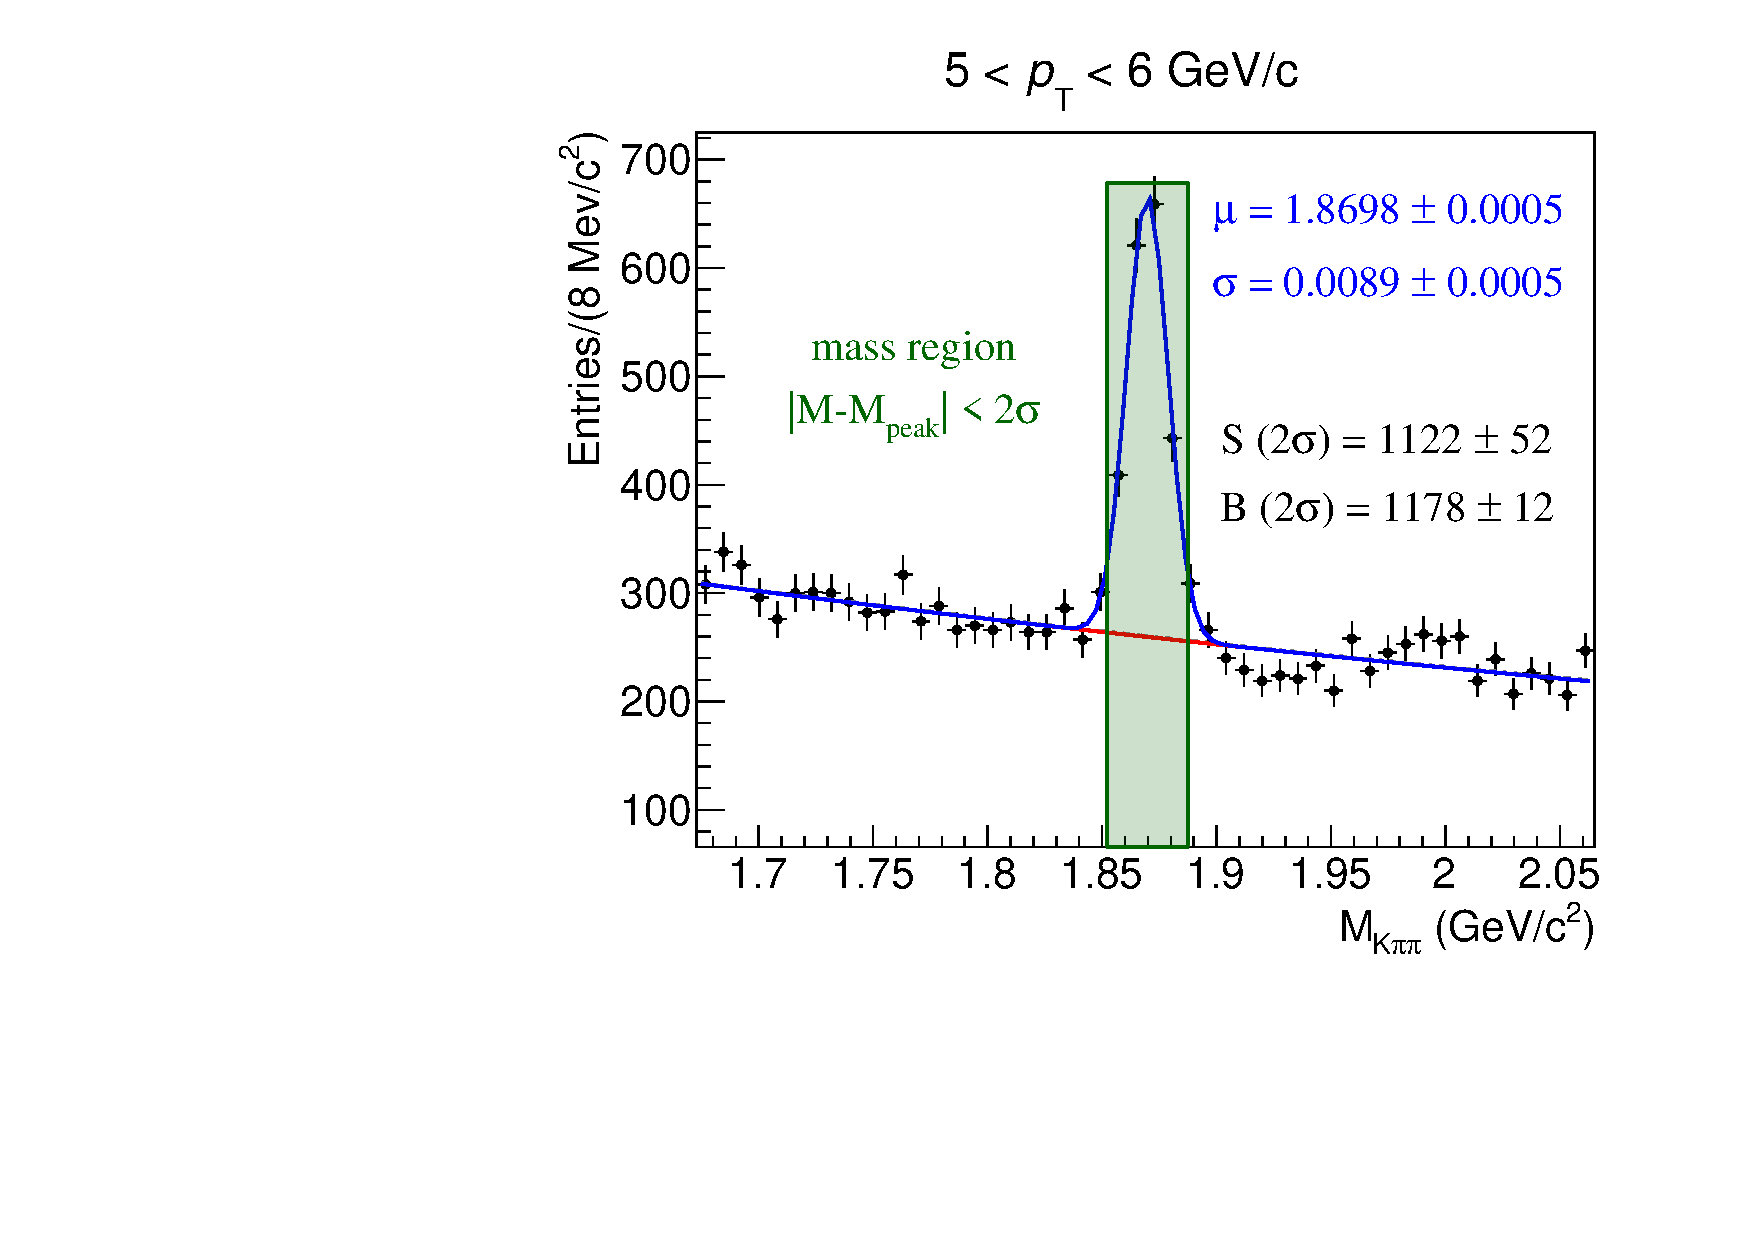
\includegraphics[scale=0.25]{Mass_5-6_fit.pdf}}
\put(150,60){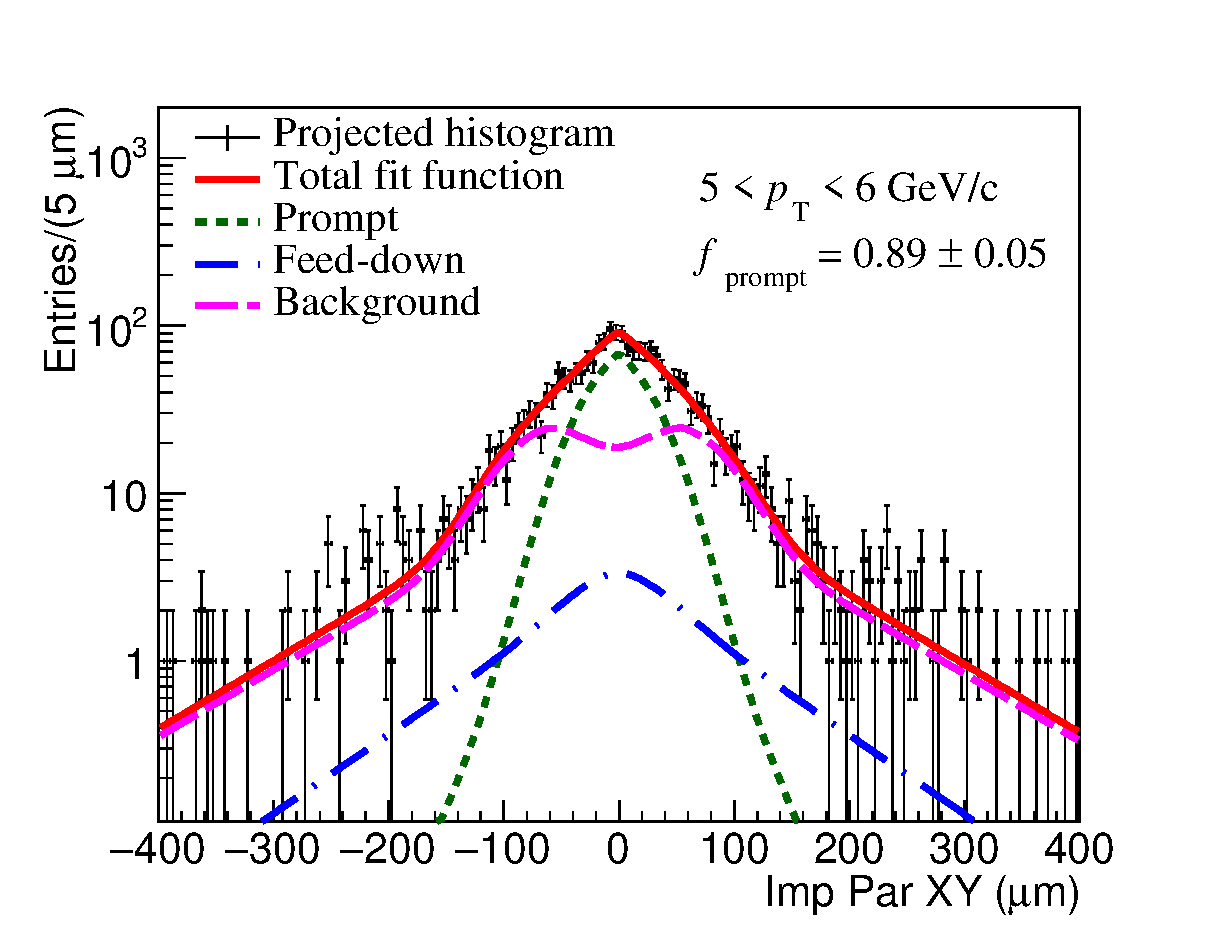
\includegraphics[scale=0.35]{FitUnbinned_5-6_bkg_plot.eps}}

\put(81,120){
\begin{tikzpicture}[->]
\draw[draw=verdebbello,solid,line width=0.3mm] (0, 0) -- + (3.,-2);
\end{tikzpicture}}

\put(160,235){\captionsetup{labelformat=empty}
\begin{minipage}[t]{0.5\linewidth}
\begin{center}
Intervallo di massa invariante considerato
\[|M-M_{peak}|<2\sigma\]
\end{center}
\end{minipage}}

\put(-5,125){\captionsetup{labelformat=empty}
\begin{minipage}[t]{0.45\linewidth}
\begin{itemize}
 \item Parametri liberi: $f_{prompt}, \text{ } \sigma_{prompt}$
 \item $S$ è fissato al valore del segnale ottenuto dal fit della massa invariante (\textit{raw yield})
 \item $N$ è fissato al numero di conteggi
\end{itemize}
\end{minipage}}

\put(15,60){\captionsetup{labelformat=empty}
\begin{minipage}[t]{0.9\linewidth}
 \begin{block}{}
 \setlength\abovedisplayskip{0pt}
\[ \textcolor{red}{F(d_0^{xy})} = N \cdot \bigg\{\frac{S}{N}\bigg{[}f_{prompt}\textcolor{verdebbello}{F^{prompt}(d_0^{xy})}+(1-f_{prompt})\textcolor{blue}{F^{feed-down}_{reco}(d_0^{xy})}\bigg{]}+\frac{N-S}{N}\textcolor{magenta}{F^{bkg}(d_0^{xy})}\bigg\} \]
\end{block}
\end{minipage}}

\end{picture} 
\end{frame}

\begin{frame}
\frametitle{Valutazione degli errori sistematici}
\begin{picture}(320,250)

\put(5,12){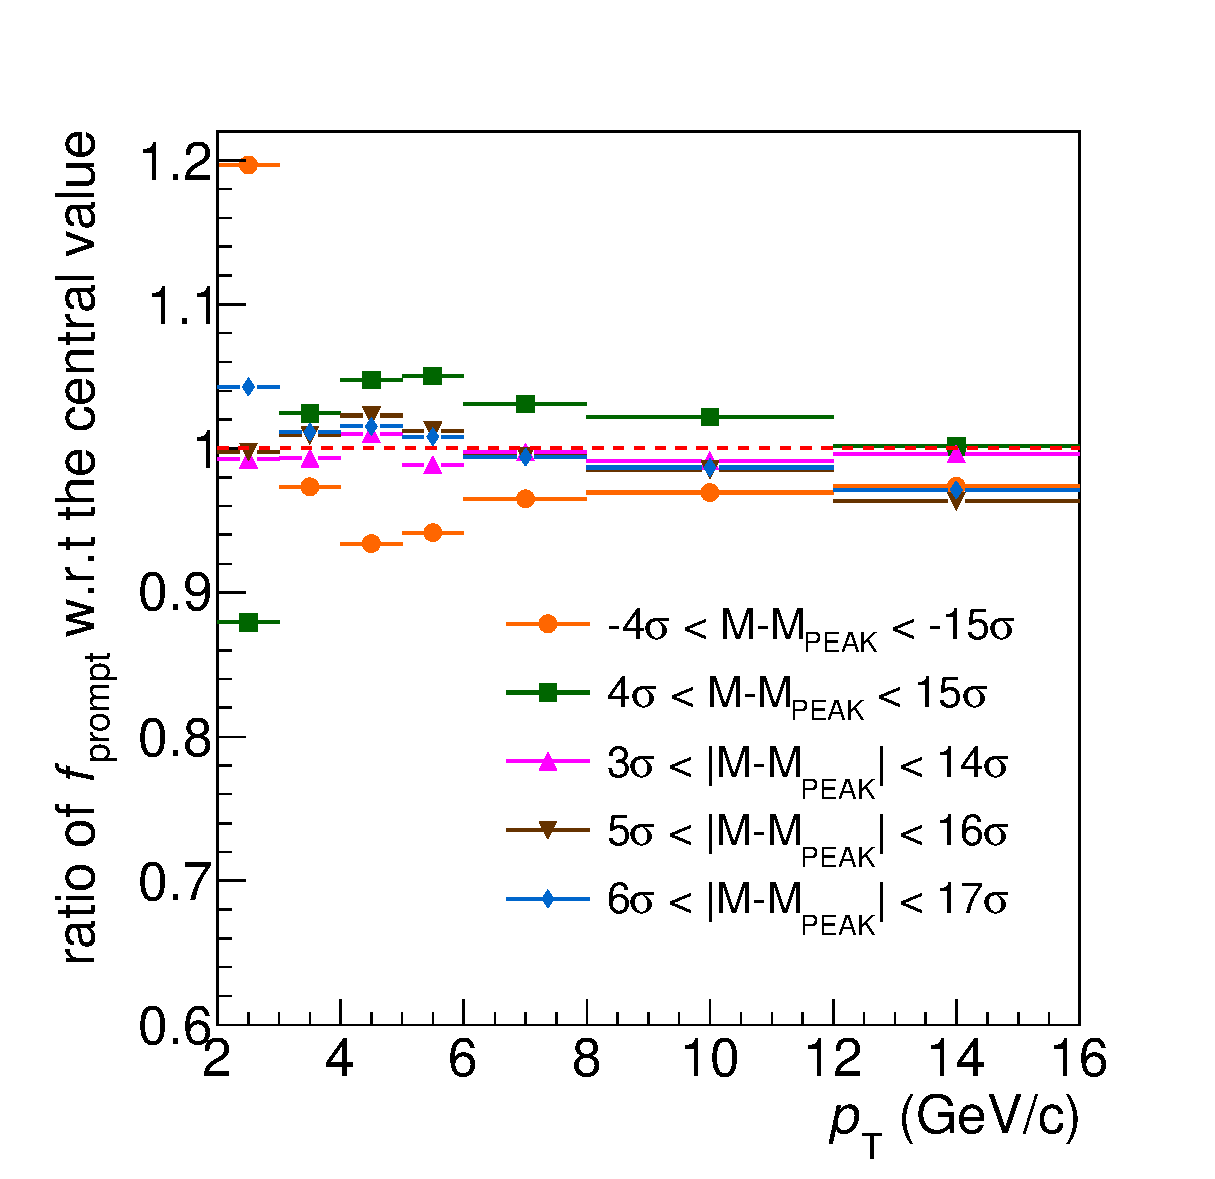
\includegraphics[scale=0.18]{promptfraction_syst_SBtot_ratioonly.eps}}
\put(125,12){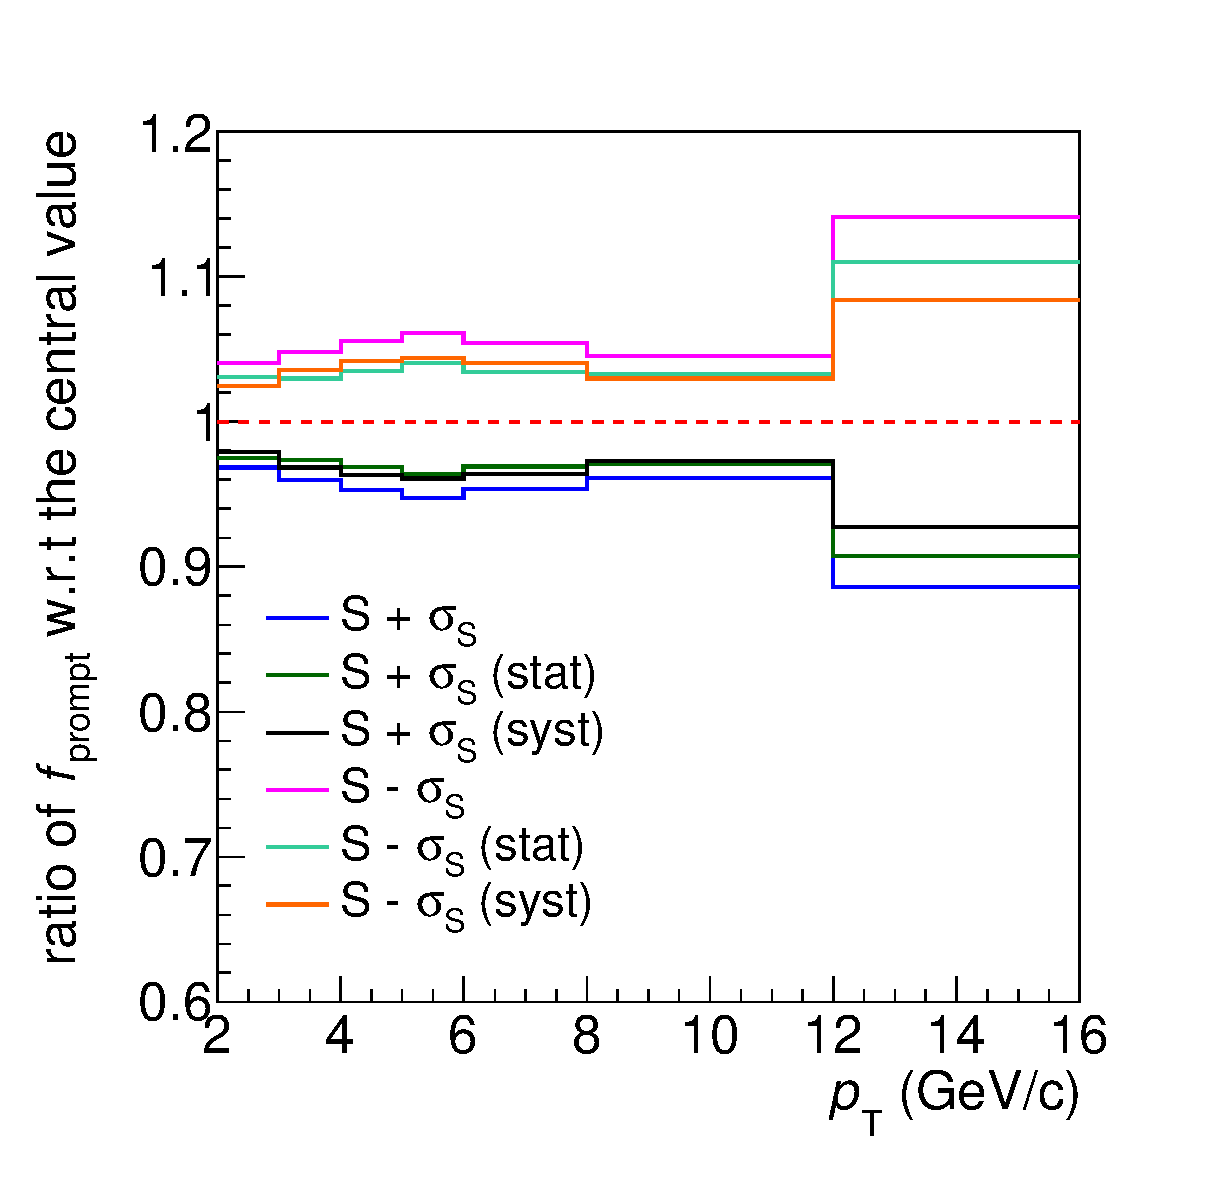
\includegraphics[scale=0.18]{promptfraction_syst_SoverT_onlyratio.eps}}
\put(240,12){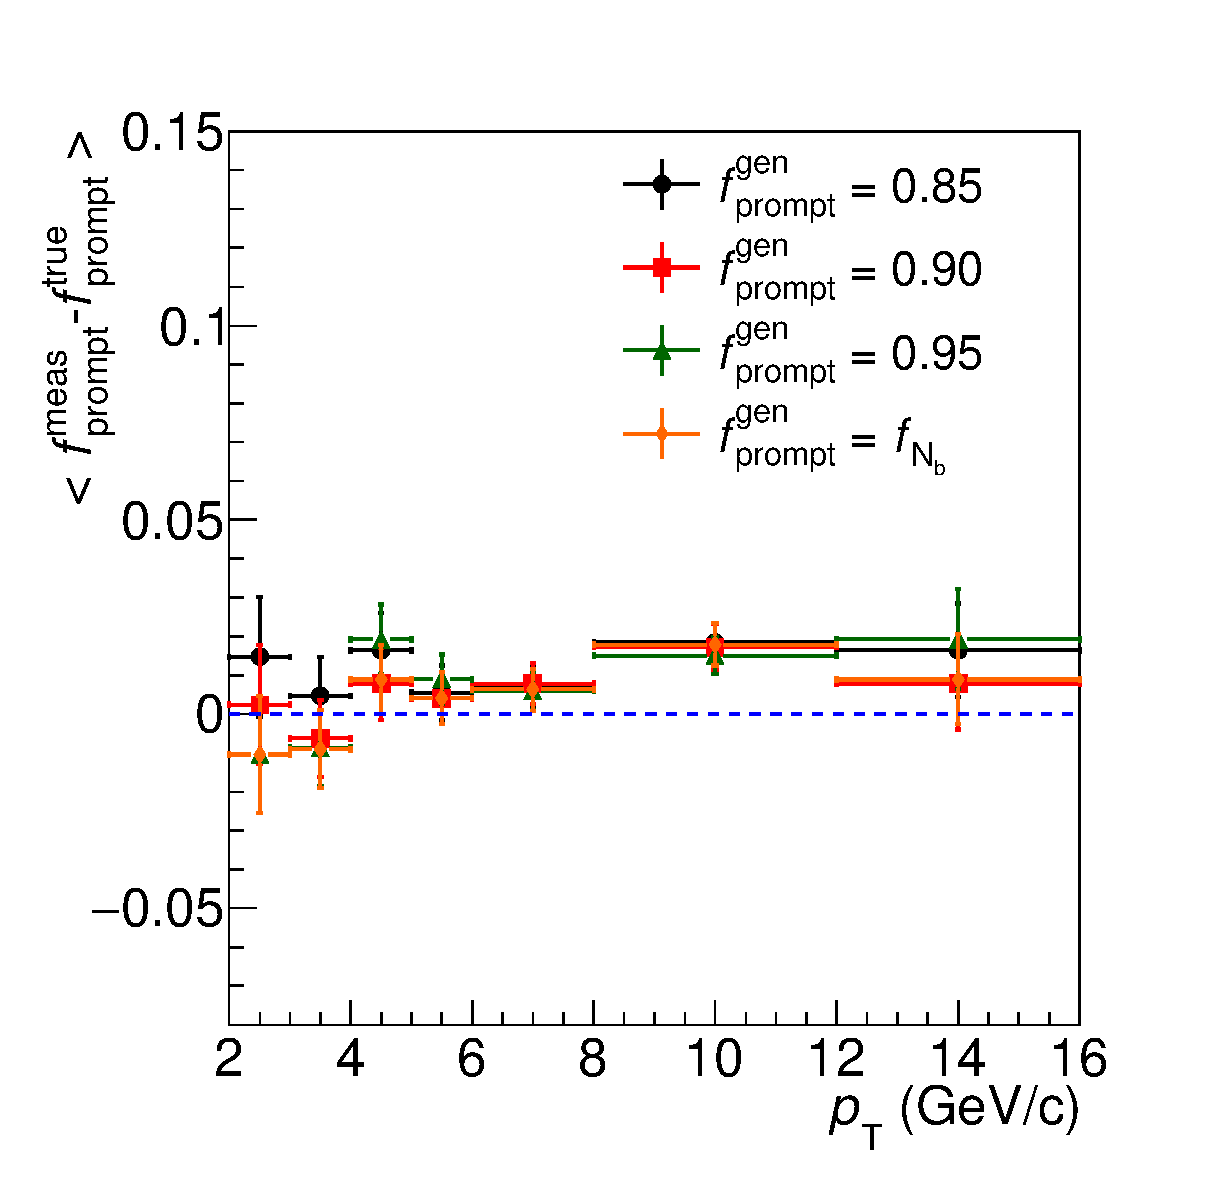
\includegraphics[scale=0.18]{Bias_bkg_freesigma.eps}}

\put(0,235){\captionsetup{labelformat=empty}
\begin{minipage}[t]{1.\linewidth}
Sorgenti di errore sistematico:
\begin{enumerate}
 \item Imperfetta descrizione delle distribuzioni 
 \begin{enumerate}[a)]
  \item Forma delle distribuzioni del parametro di impatto di D$^+$ prompt e feed-down nella simulazione Monte Carlo e del fondo combinatoriale nelle side-bands \\
 \item Forma delle distribuzioni di $\pt$ di mesoni D$^+$ e B generati nella simulazione Monte Carlo \\
 \end{enumerate}
 \item Incertezza sulla valore del segnale $S$
 \item Consistenza e stabilità del procedimento
\end{enumerate}
\end{minipage}}

\put(-5,150){\captionsetup{labelformat=empty}
\begin{minipage}[t]{0.3\linewidth}
\begin{enumerate}
\item Variazione del range di massa invariante per la parametrizzazione del fondo
\end{enumerate}
\end{minipage}}

\put(112,150){\captionsetup{labelformat=empty}
\begin{minipage}[t]{0.3\linewidth}
\begin{enumerate} 
\setcounter{enumi}{1}
\item Variazione della quantità di segnale $S$ nel fit tra $S-\sigma_S$ e $S+\sigma_S$
\end{enumerate}
\end{minipage}}

\put(235,150){\captionsetup{labelformat=empty}
\begin{minipage}[t]{0.3\linewidth}
\begin{enumerate}
\setcounter{enumi}{2}
\item Test Monte Carlo per valutare la bontà del procedimento
\end{enumerate}
\end{minipage}}

\end{picture} 
\end{frame}

\begin{frame}
\frametitle{Fit del parametro di impatto - Risultato}
\begin{picture}(320,250)

\put(0,20){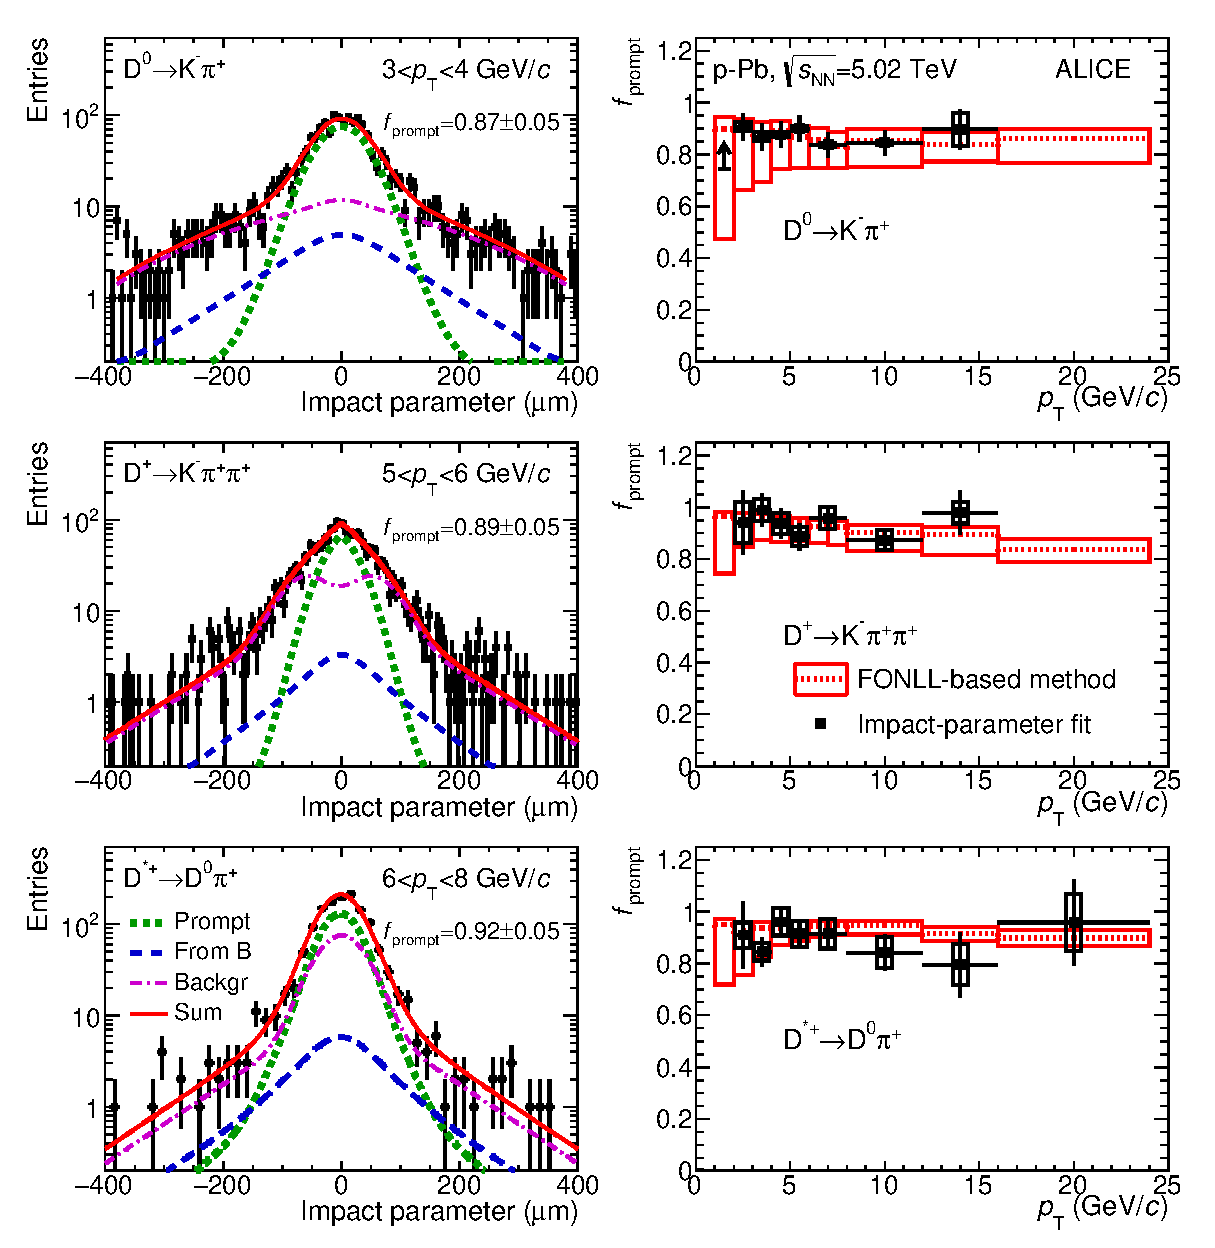
\includegraphics[scale=0.37]{ImpParFitAndRes.eps}}

\put(-5,91){
\begin{tikzpicture}[-]
\draw[draw=blue,solid,line width=0.3mm] (0, 0) -- + (7.6,0);
\end{tikzpicture}}

\put(-5,163){
\begin{tikzpicture}[-]
\draw[draw=blue,solid,line width=0.3mm] (0, 0) -- + (7.6,0);
\end{tikzpicture}}

\put(-5,91){
\begin{tikzpicture}[-]
\draw[draw=blue,solid,line width=0.3mm] (0, 0) -- + (0,2.54);
\end{tikzpicture}}

\put(211,91){
\begin{tikzpicture}[-]
\draw[draw=blue,solid,line width=0.3mm] (0, 0) -- + (0,2.54);
\end{tikzpicture}}

\put(211,210){\captionsetup{labelformat=empty}
\begin{minipage}[t]{0.38\linewidth}
\begin{itemize}
 \item La frazione di D$^+$ prompt misurata con il metodo del fit del parametro di impatto è compatibile con i metodi \textit{theory-driven}
 \item L'incertezza totale è compatibile con i metodi \textit{theory-driven} a $\pt$ intermedio e maggiore ad alto e basso $\pt$
 \item Risultato inserito come cross-check nell'articolo \textcolor{blue}{\textit{D-meson production in p-Pb collisions at $\sqrt{s_{NN}}=5.02$ TeV and in pp collisions at $\sqrt{s}=7$ TeV}} pubblicato dalla Collaborazione ALICE 
\end{itemize}
\end{minipage}}

\end{picture} 
\end{frame}

\section{Metodo della variazione dei tagli}
\begin{frame}
\frametitle{Metodo della variazione dei tagli}
\begin{picture}(320,250)

\put(145,86){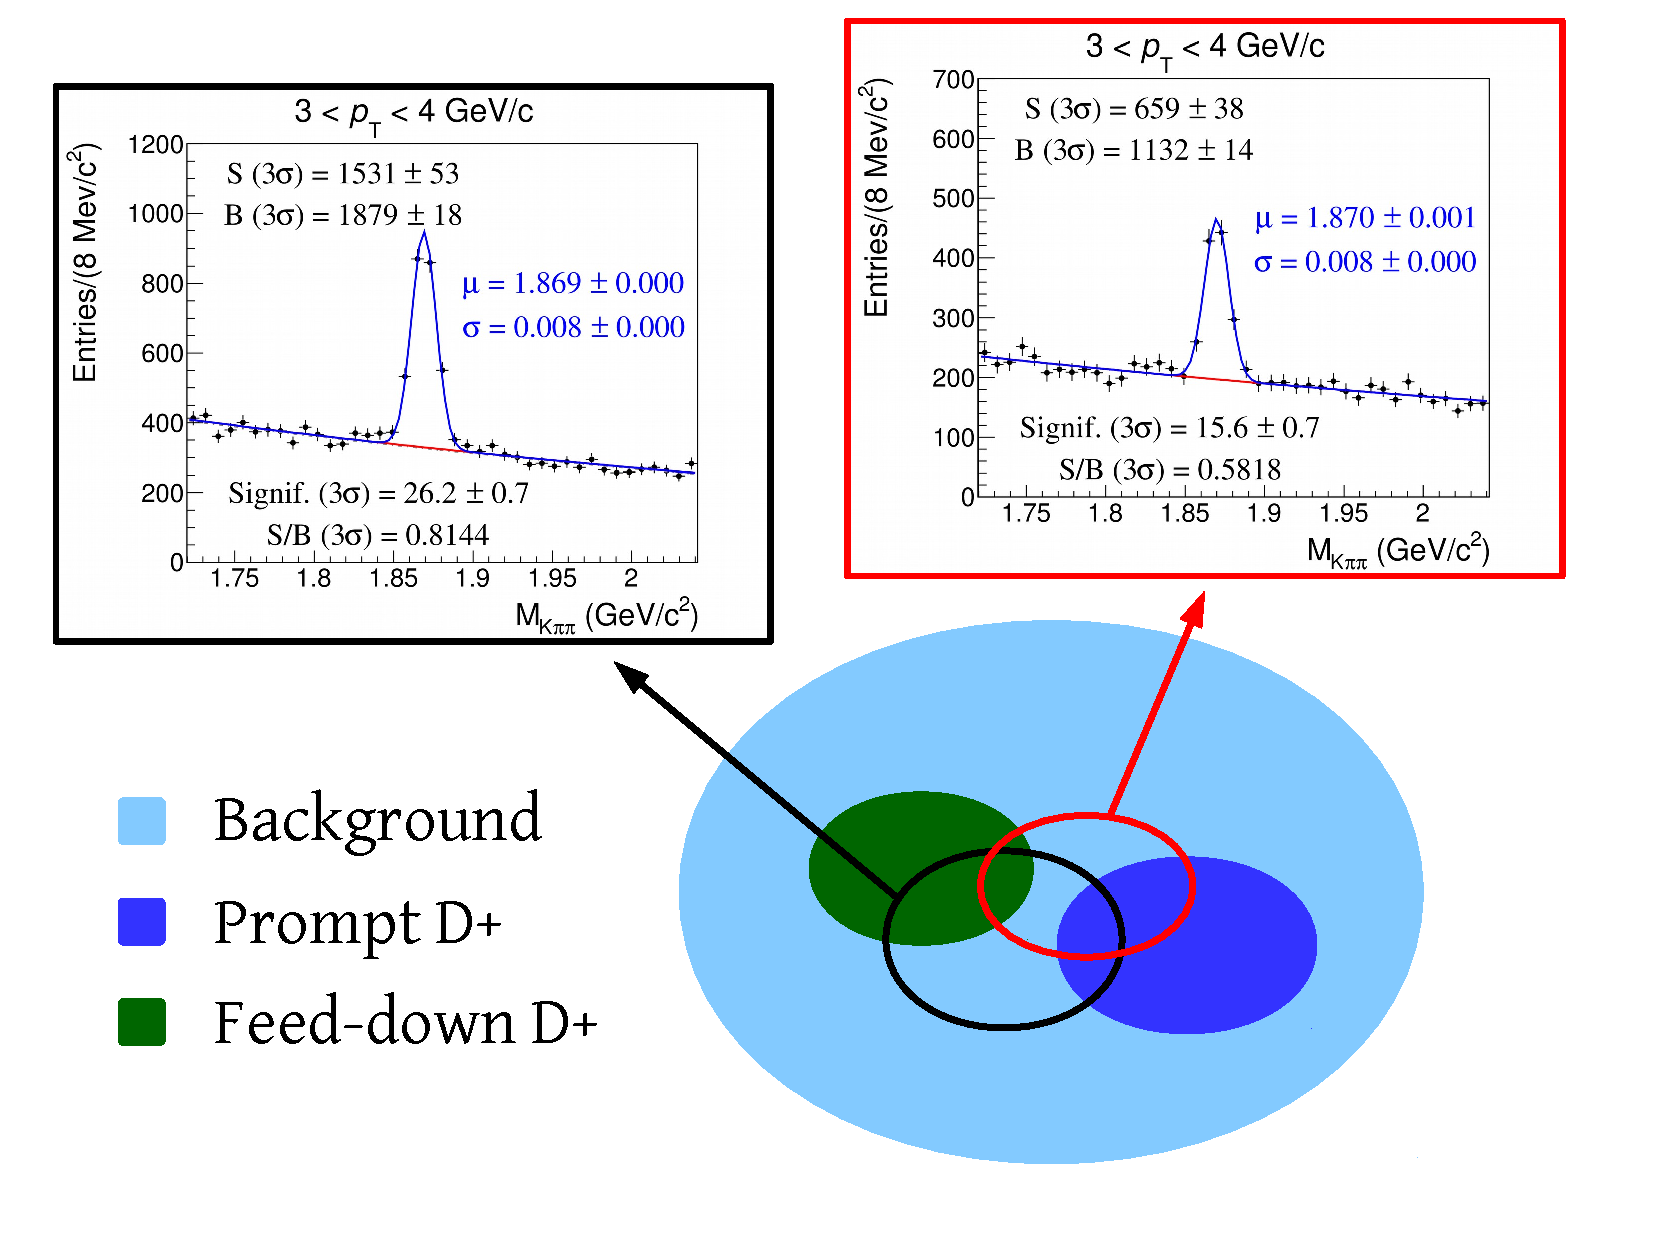
\includegraphics[scale=0.27]{cutvar_sketch.pdf}}

\put(0,220){\captionsetup{labelformat=empty}
\begin{minipage}[t]{0.4\linewidth}
\begin{center}
I candidati mesoni D$^+$ includono D$^+$ prompt, D$^+$ feed-down e il fondo combinatoriale \\[3mm]
Applicando selezioni su quantità topologiche per massimizzare il rapporto segnale su fondo e la significatività statistica \[signif. = \frac{S}{\sqrt{S+B}},\] se ne seleziona soltanto una parte
\end{center}
\end{minipage}}

\put(187,82){\captionsetup{labelformat=empty}
\begin{minipage}[t]{0.45\linewidth}
\begin{center}
Per ogni set di tagli definito si ottiene un'equazione che ha come incognite il numero corretto di mesoni D$^+$ prompt e feed-down ($N_{prompt}$ e $N_{feed-down}$) \\[2mm] $\Rightarrow$ per $n$ set di tagli si ottiene un sistema sovradeterminato
\end{center}
\end{minipage}}

\put(3,93){\captionsetup{labelformat=empty}
\begin{minipage}[t]{0.49\linewidth}
\begin{block}{}
\setlength\abovedisplayskip{0pt}
\begin{equation*}
\begin{cases}
\epsilon^{prompt}_1\cdot N_{prompt} + \epsilon^{feed-down}_1\cdot N_{feed-down} = Y_1\\
..\\
..\\
\epsilon^{prompt}_n\cdot N_{prompt} + \epsilon^{feed-down}_n\cdot N_{feed-down} = Y_n\\
\end{cases}
\label{cutvar_syst}
\end{equation*}
\end{block}
\end{minipage}}

\end{picture}
\end{frame}

\begin{frame}
\frametitle{Metodi di minimizzazione}
\begin{picture}(320,250)

\put(-5,5){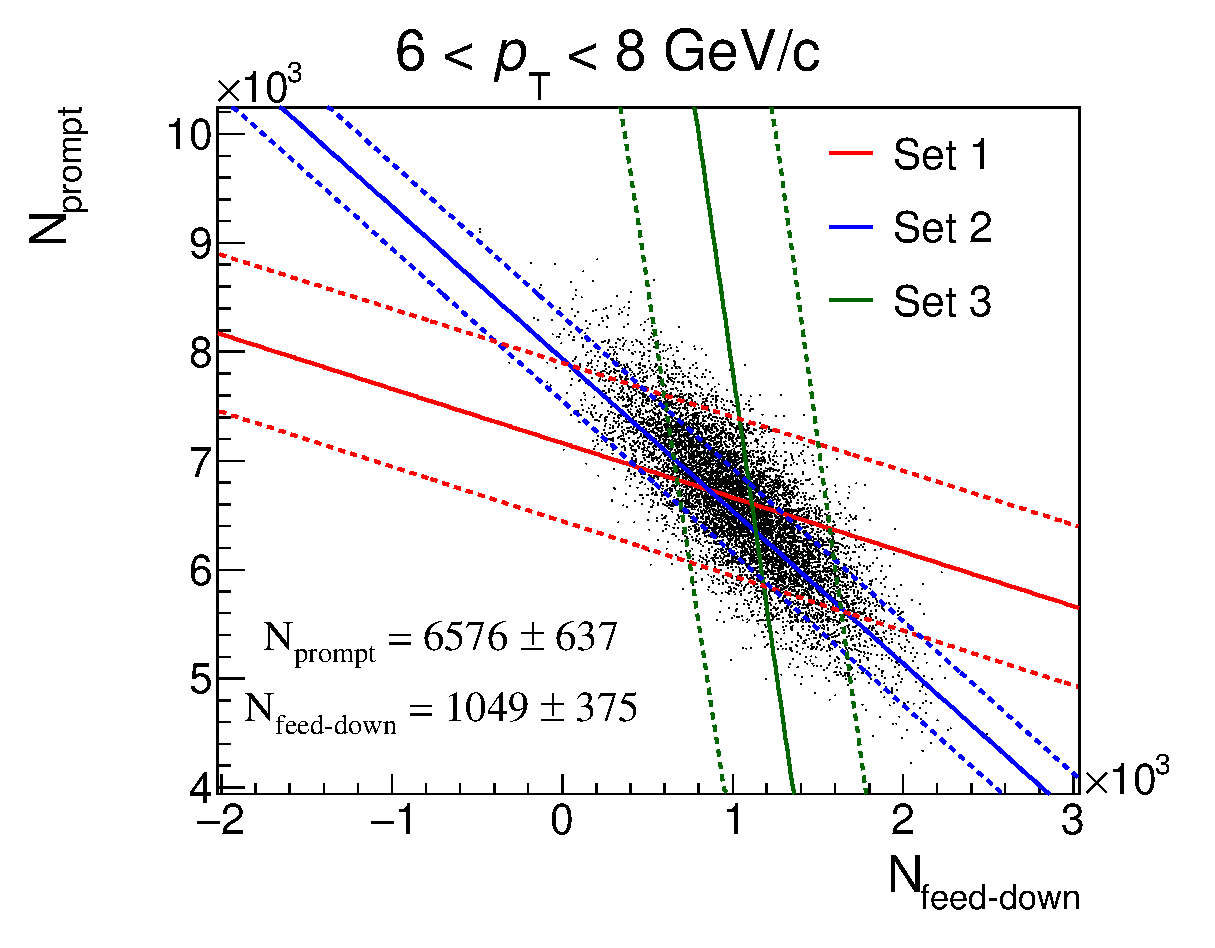
\includegraphics[scale=0.24]{LinesDisp_6-8.eps}}

\put(0,234){\captionsetup{labelformat=empty}
\begin{minipage}[t]{0.7\linewidth}
\begin{equation*}
\renewcommand\arraystretch{1.3} {
\left(
\begin{array}{cc}
\epsilon^{prompt}_1 & \epsilon^{feed-down}_1\\
\epsilon^{prompt}_2 & \epsilon^{feed-down}_2\\
.. & ..\\
\epsilon^{prompt}_n & \epsilon^{feed-down}_n
\end{array}
 \right)} 
 \times
 \left(
\begin{array}{c}
 N_{prompt}\\
 N_{feed-down}
\end{array}
 \right) 
 -
  \left(
\begin{array}{c}
Y_1\\
Y_2\\
..\\
Y_n
\end{array}
 \right)
 = \textcolor{red}{
\left(
\begin{array}{c}
\delta_1\\
\delta_2\\
..\\
\delta_n
\end{array}
 \right)}
\end{equation*} 
\end{minipage}}

\put(250,220){\captionsetup{labelformat=empty}
\begin{minipage}[t]{0.25\linewidth}
\begin{center}
Il vettore nullo è sostituito dal vettore dei residui $\pmb{\textcolor{red}{\delta}}$
\end{center}
\end{minipage}}

\put(0,160){\captionsetup{labelformat=empty}
\begin{minipage}[t]{0.6\linewidth}
Il numero corretto di mesoni D$^+$ prompt e feed-down e la matrice delle covarianze associata sono ottenuti dalla minimizzazione del $\chi^2 = \pmb{\delta}^T \pmb{C}^{-1} \pmb{\delta}$ 
\end{minipage}}

\put(180,175){\captionsetup{labelformat=empty}
\begin{minipage}[t]{0.6\linewidth}
\[
\pmb{C} = 
\left(
\begin{array}{cccc}
\sigma^2_{\delta_1} & & &\\
 & \sigma^2_{\delta_2} & &\\
 & & \ddots &\\
 &  &  & \sigma^2_{\delta_n}
\end{array}
 \right) 
\]
\end{minipage}}

\put(0,240){\captionsetup{labelformat=empty}
\begin{minipage}[t]{0.5\linewidth}
\begin{itemize}
 \item \textcolor{blue}{Minimizzazione analitica} \\[3.7cm]
 \item \textcolor{blue}{Determinazione dell'incentro}
\end{itemize}
\end{minipage}}

\put(135,95){\captionsetup{labelformat=empty}
\begin{minipage}[t]{0.6\linewidth}
Ogni equazione corrispondente ad un set di tagli descrive una retta nel piano $(N_{prompt}, N_{feed-down})$\\ $\Rightarrow$ le intersezioni di tre rette definiscono un triangolo \\$\Rightarrow$ $N_{prompt}$ e $N_{feed-down}$ sono determinati dalle coordinate dell'incentro del triangolo \\[2mm]
L'errore statistico è valutato con una simulazione Monte Carlo, estraendo i parametri delle rette da delle distribuzioni Gaussiane 
\end{minipage}}

\end{picture}
\end{frame}

\begin{frame}
\frametitle{Strategia per la scelta dei set di tagli}
\begin{picture}(320,250)

\put(-5,15){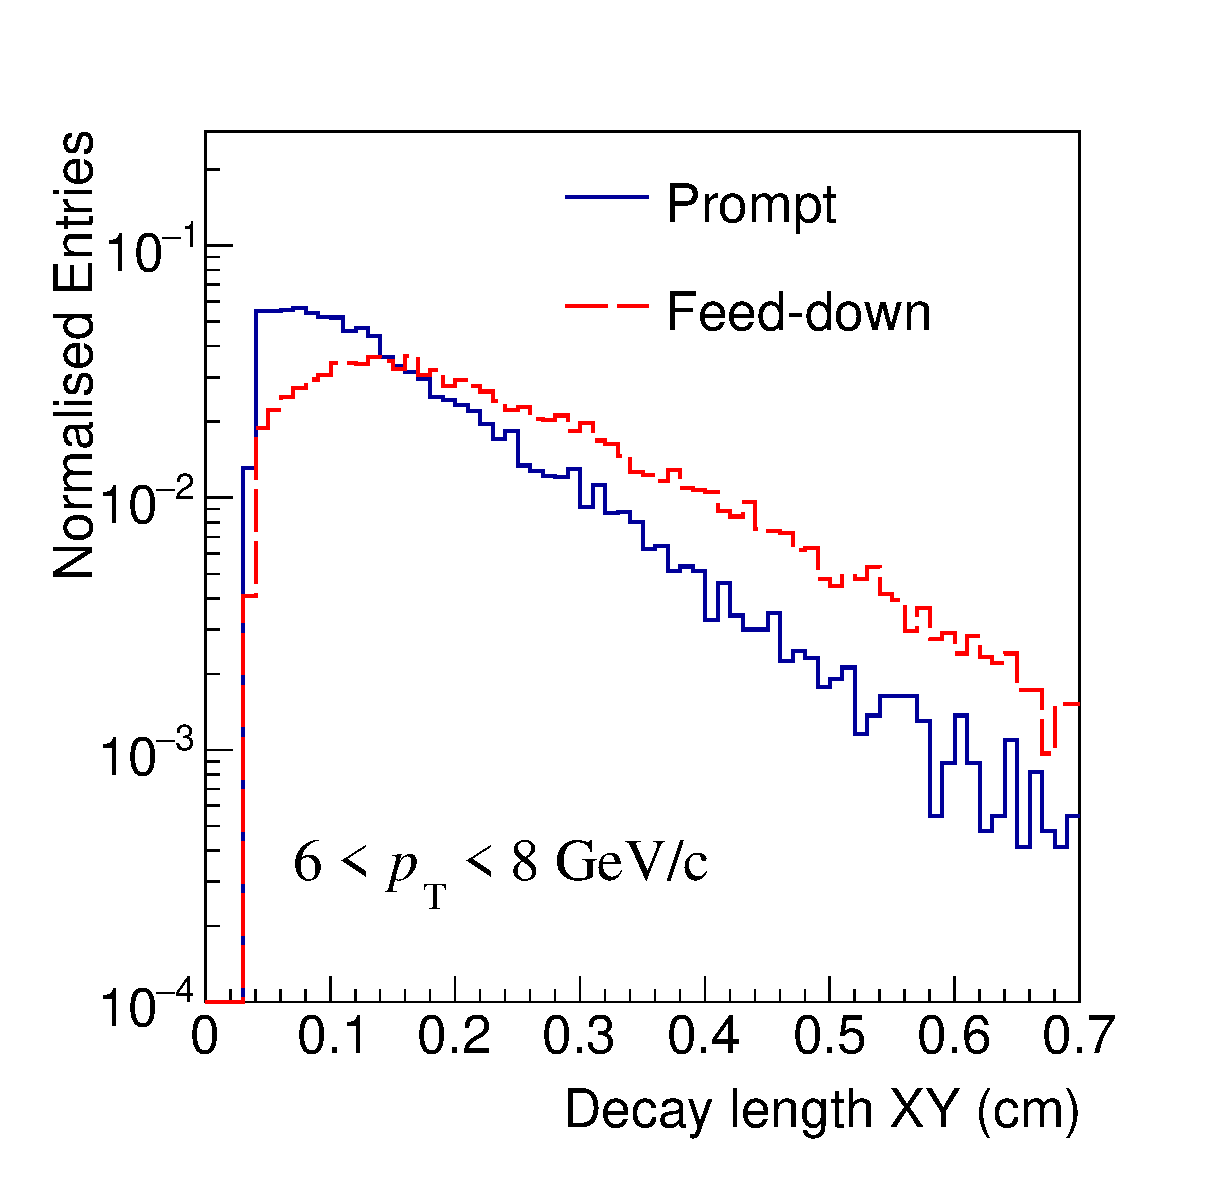
\includegraphics[scale=0.16]{CompPromptFD_DLXY_6-8.eps}}
\put(83,15){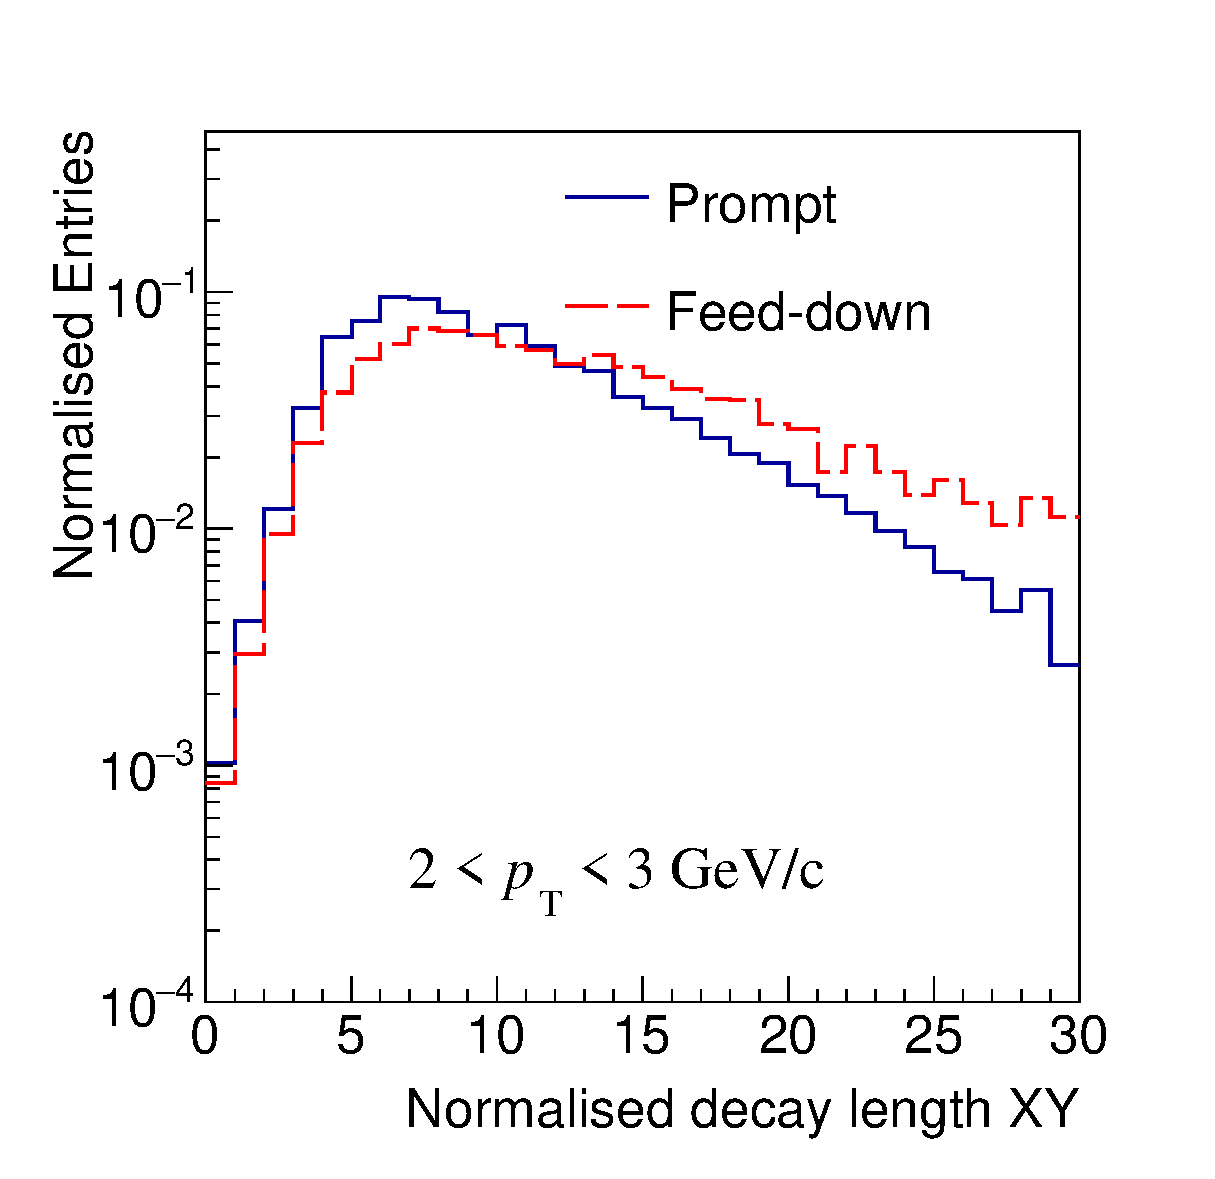
\includegraphics[scale=0.16]{CompPromptFD_NDLXY_2-3.eps}}
\put(176,15){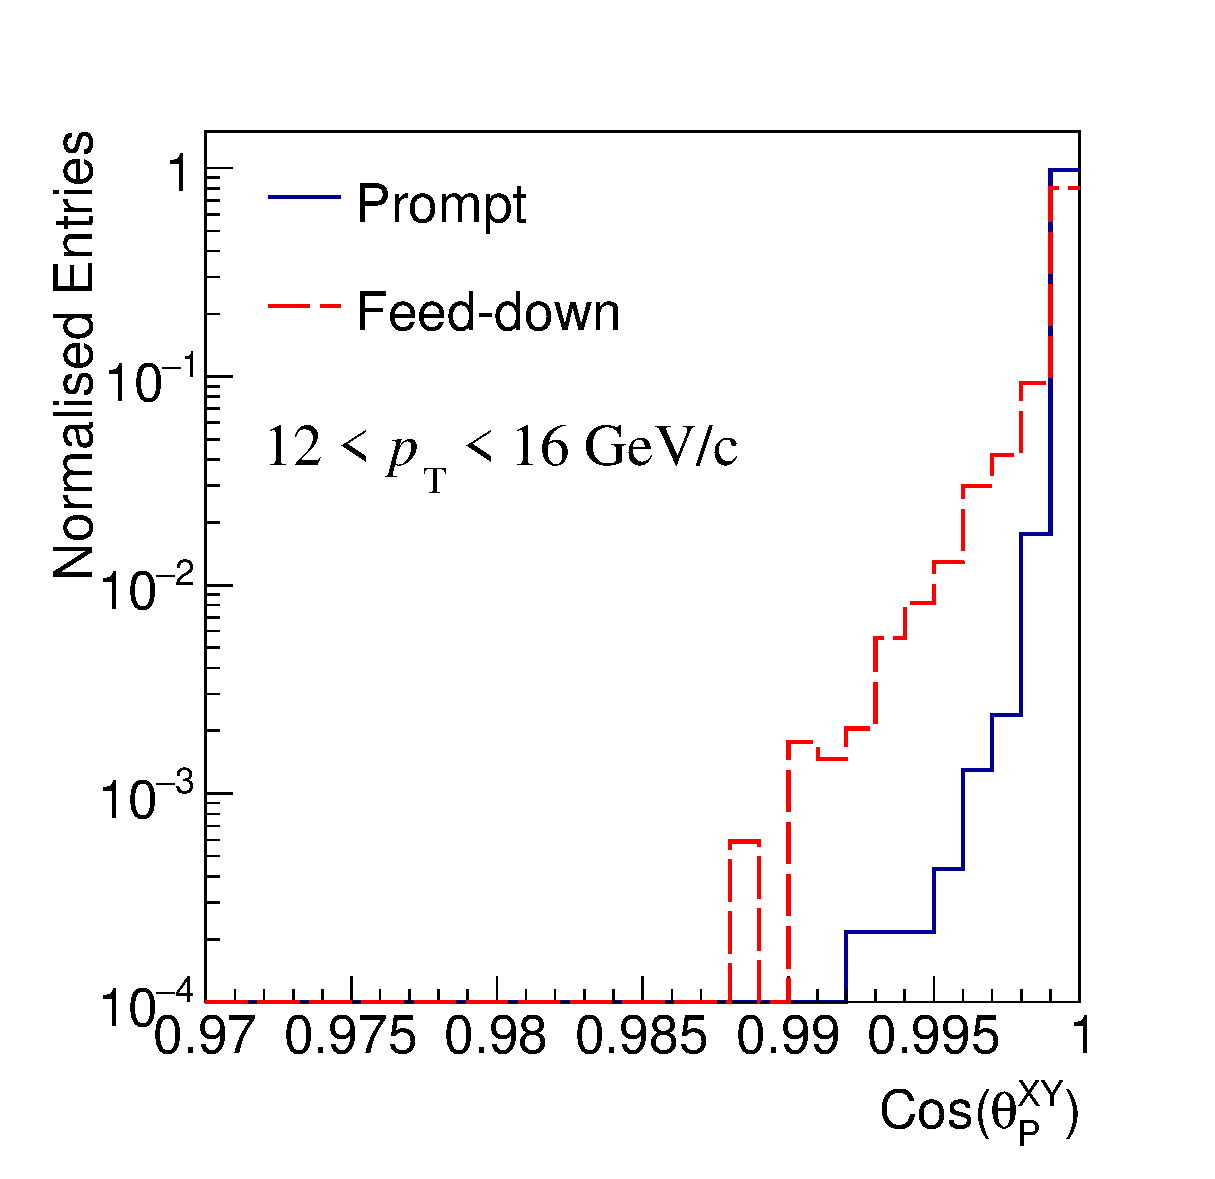
\includegraphics[scale=0.16]{CompPromptFD_CospXY_12-16.eps}}
\put(264,15){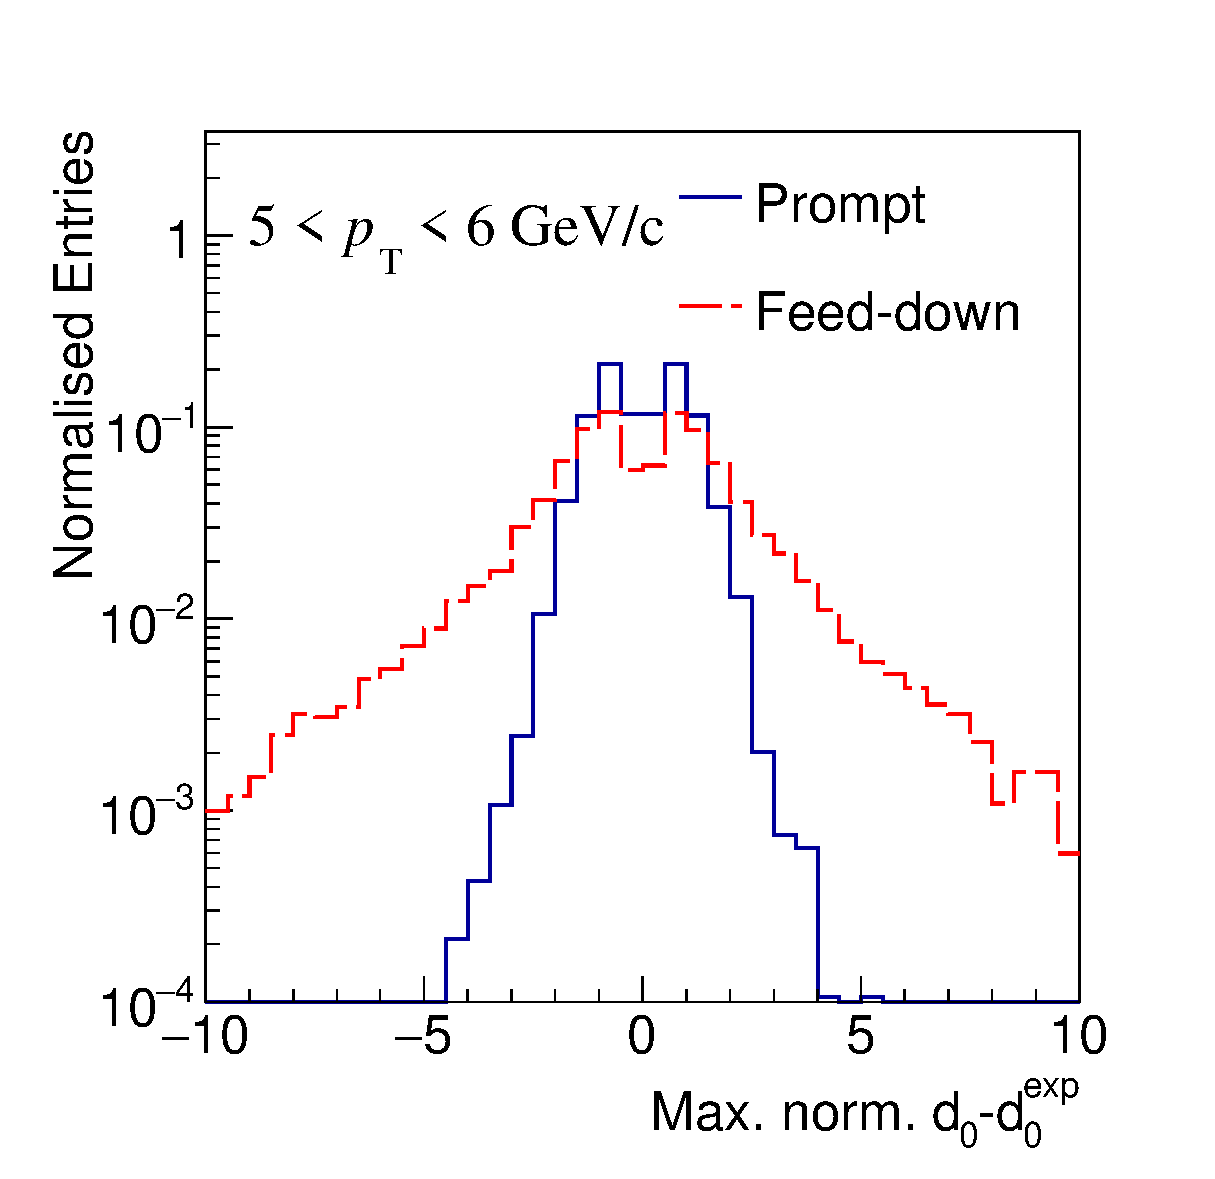
\includegraphics[scale=0.16]{CompPromptFD_d0d0exp_5-6.eps}}

\put(0,235){\captionsetup{labelformat=empty}
\begin{minipage}[t]{1.\linewidth}
Sono stati utilizzati tre set di tagli il più possibile \textcolor{blue}{scorrelati}:\\[2.3cm]
Variabili topologiche usate per definire i set di tagli:
\end{minipage}}

\put(25,231){
\begin{minipage}[t]{0.85\linewidth}
\begin{block}{}
\setlength\abovedisplayskip{0pt}
\begin{itemize}
 \item 1$^o$ set: aumento dell'efficienza di selezione dei mesoni D$^+$ prompt 
 \item 2$^o$ set: intermedio (buon estrazione del segnale)
 \item 3$^o$ set: aumento dell'efficienza di selezione dei mesoni D$^+$ feed-down
\end{itemize}
\end{block}
\end{minipage}}

\put(0,145){
\begin{minipage}[t]{0.25\linewidth}
\begin{itemize}
 \item Lunghezza di decadimento nel piano trasverso
\end{itemize}
\end{minipage}}

\put(85,145){
\begin{minipage}[t]{0.25\linewidth}
\begin{itemize}
 \item Lunghezza di decadimento nel piano trasverso normalizzata al proprio errore
\end{itemize}
\end{minipage}}

\put(175,145){
\begin{minipage}[t]{0.25\linewidth}
\begin{itemize}
 \item Coseno dell'\\angolo di \\pointing nel \\piano trasverso
\end{itemize}
\end{minipage}}

\put(260,155){
\begin{minipage}[t]{0.25\linewidth}
\begin{itemize}
 \item Massima differenza normalizzata tra il parametro di impatto atteso e misurato delle tracce figlie
\end{itemize}
\end{minipage}}

\end{picture}
\end{frame}

\begin{frame}
\frametitle{Metodo della variazione dei tagli\\ Risultato}
\begin{picture}(320,250)

\put(-5,88){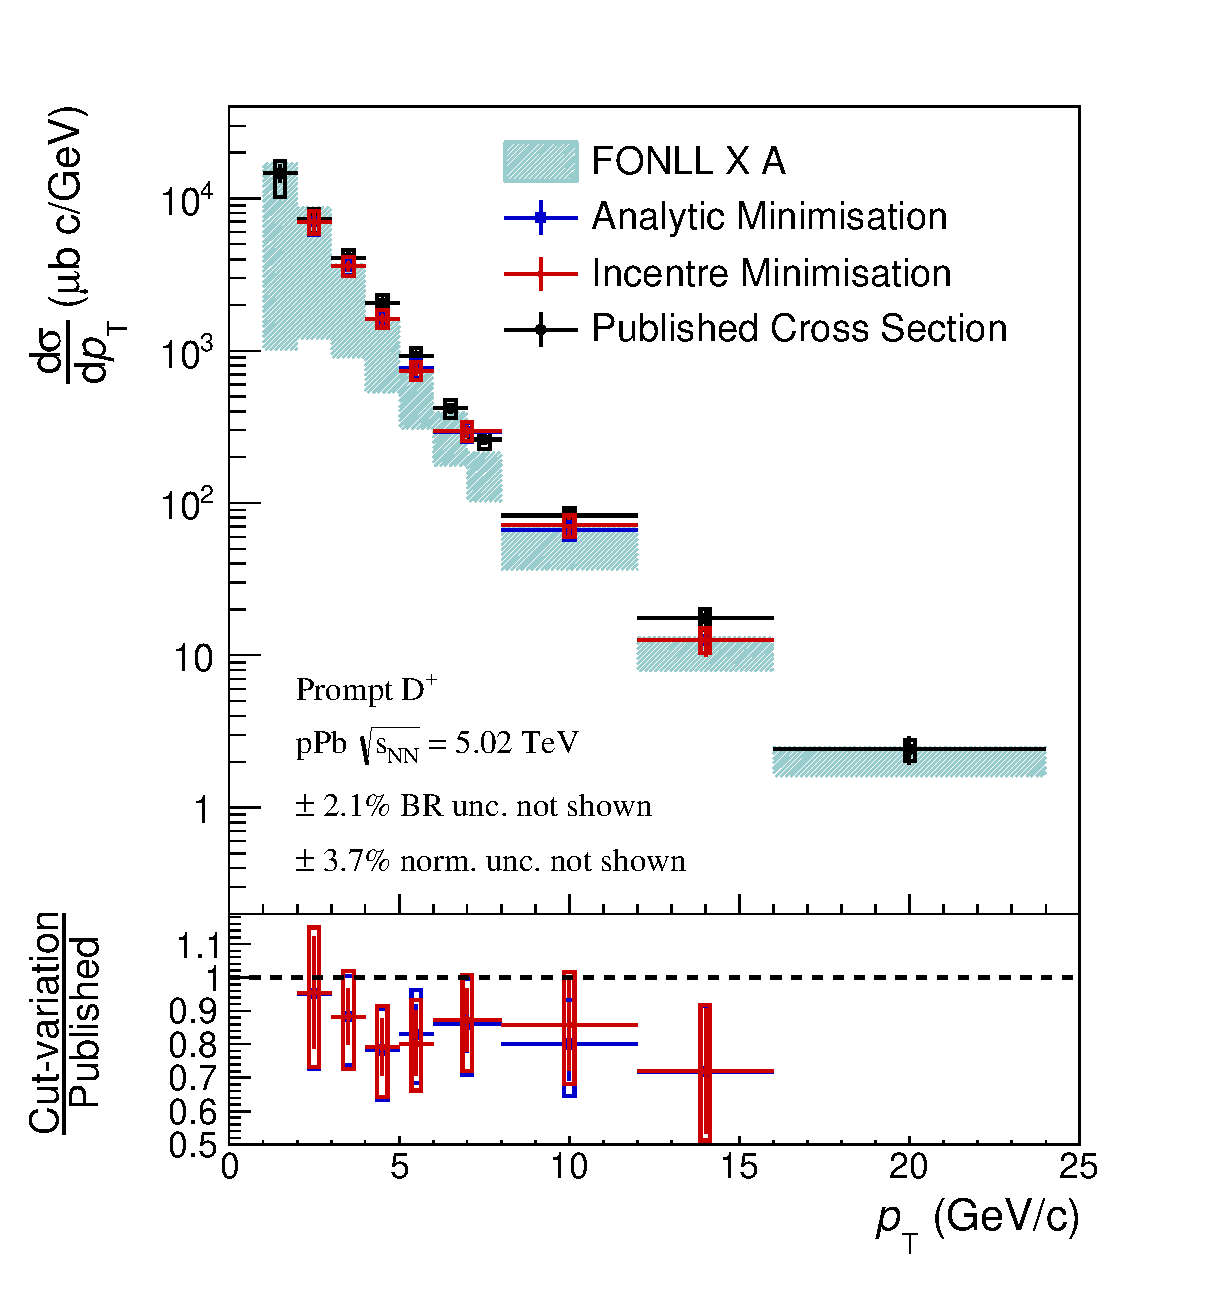
\includegraphics[scale=0.25]{CrossSectionPromptpPb.eps}}
\put(130,91){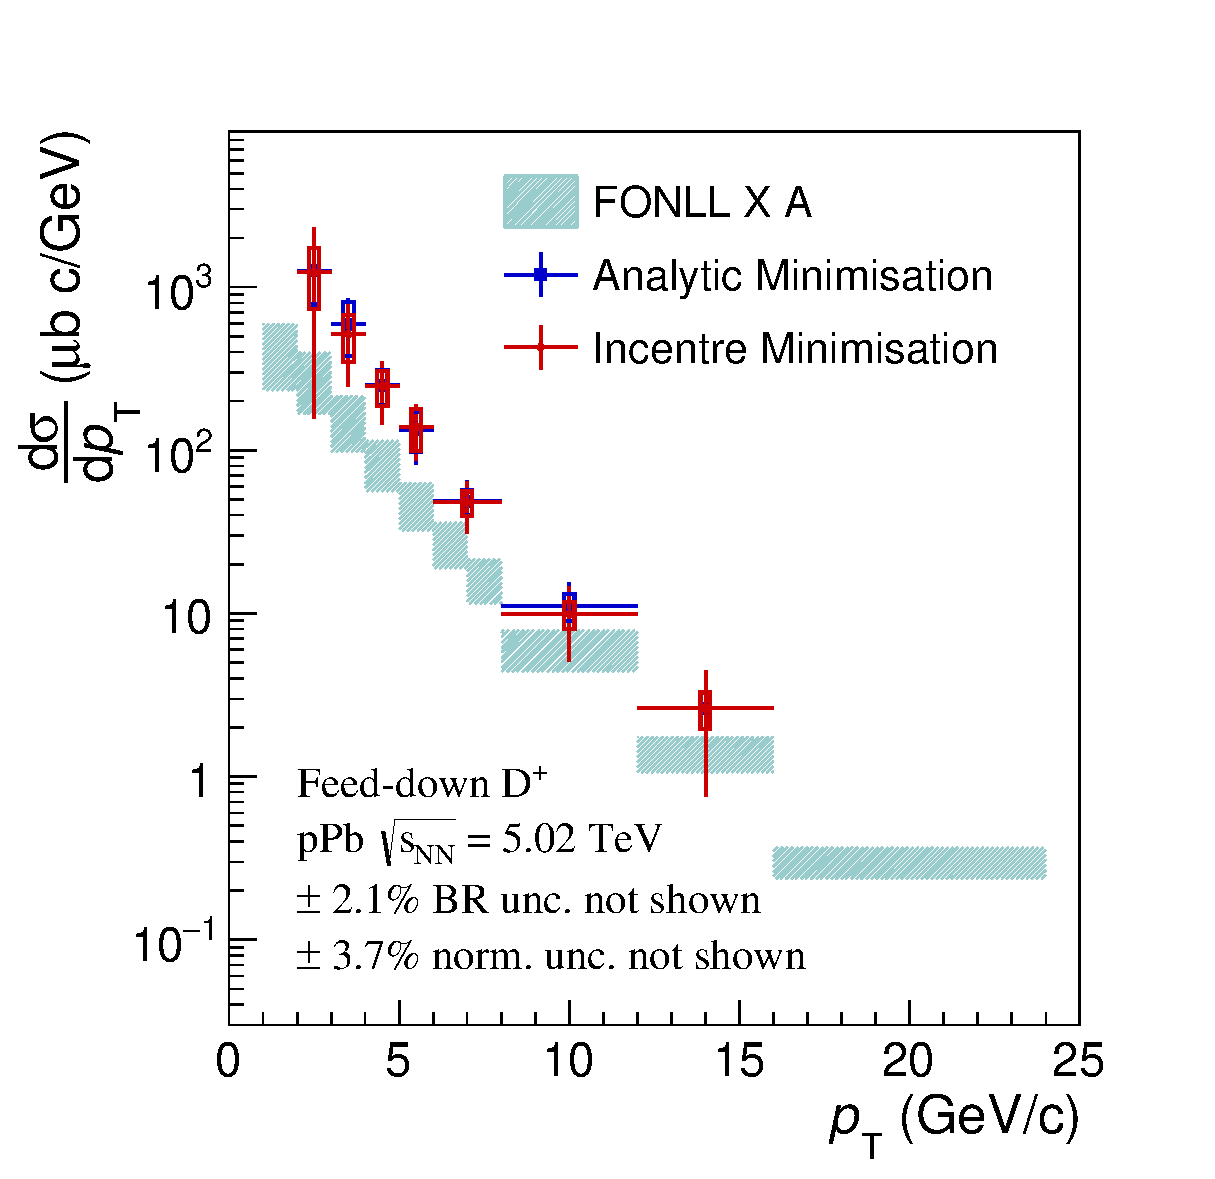
\includegraphics[scale=0.24]{CrossSectionFDpPb.eps}}

\put(175,280){\captionsetup{labelformat=empty}
\begin{minipage}[t]{0.45\linewidth}
\begin{block}{}
\setlength\abovedisplayskip{0pt}
\begin{equation*}
\frac{d\sigma^{D^+}_X}{d\pt}\bigg{|}_{|y|<0.5} = \frac{1}{2}\cdot \frac{N^{D^\pm}_X|_{|y|<y_{fid}}}{\Delta \pt \Delta y \cdot(Acc)_X} \cdot\frac{L_{int}}{BR}
\end{equation*}
\end{block} 
\end{minipage}}

\put(258,210){\captionsetup{labelformat=empty}
\begin{minipage}[t]{0.25\linewidth}
Sorgenti di errore \\sistematico:
\begin{itemize}
 \item Estrazione del segnale 
 \item Efficienza di selezione dei tagli topologici
 \item Imperfetta descrizione delle distribuzioni di $\pt$ \\di mesoni D$^+$ e B generati nella simulazione \\Monte Carlo
\end{itemize}
\end{minipage}}

\put(20,235){\captionsetup{labelformat=empty}
\begin{minipage}[t]{0.25\linewidth}
\textcolor{blue}{D$^+$ prompt}
\end{minipage}}

\put(155,213){\captionsetup{labelformat=empty}
\begin{minipage}[t]{0.25\linewidth}
\textcolor{blue}{D$^+$ feed-down}
\end{minipage}}

\put(-5,85){\captionsetup{labelformat=empty}
\begin{minipage}[t]{0.75\linewidth}
\begin{itemize}
 \item La sezione d'urto differenziale in $\pt$ di produzione dei mesoni D$^+$ prompt $\Rightarrow$ compatibile con il risultato pubblicato e la predizione di FONLL 
 \item La sezione d'urto differenziale in $\pt$ di produzione dei mesoni D$^+$ feed-down $\Rightarrow$ sistematicamente maggiore rispetto alla predizione di FONLL  
\end{itemize}
\end{minipage}}

\end{picture}
\end{frame}

\section{Ricostruzione dei mesoni D$^+$ con il filtro di Kalman}
\begin{frame}
\frametitle{Ricostruzione dei mesoni D$^+$ con il filtro di Kalman}
\begin{picture}(320,250)

\put(135,15){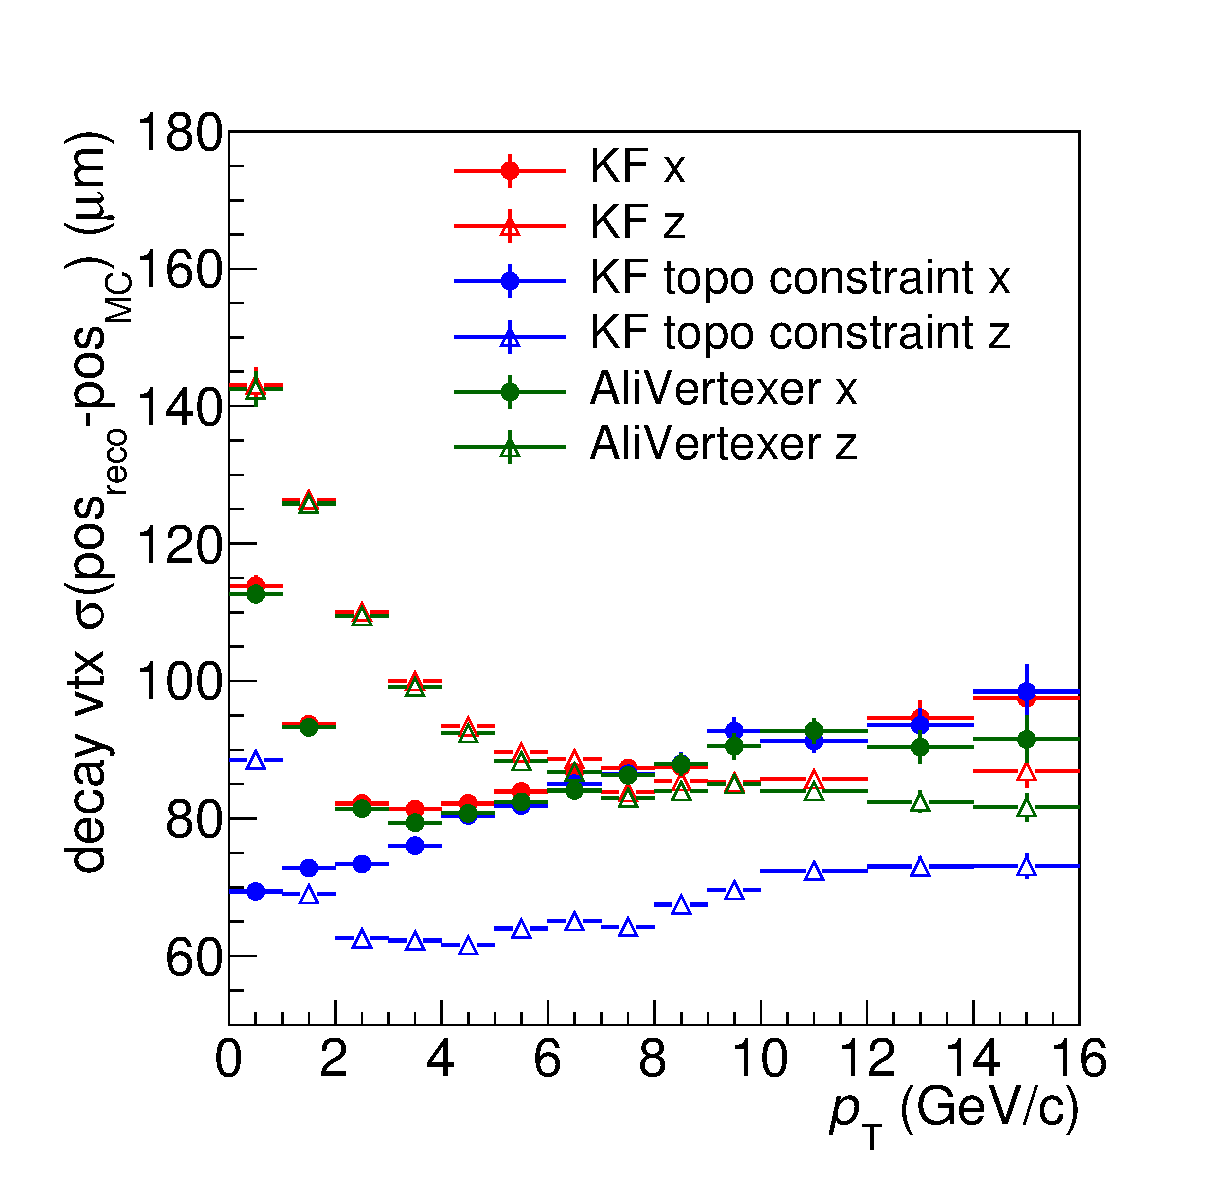
\includegraphics[scale=0.18]{ResSVXZ.eps}}
\put(240,15){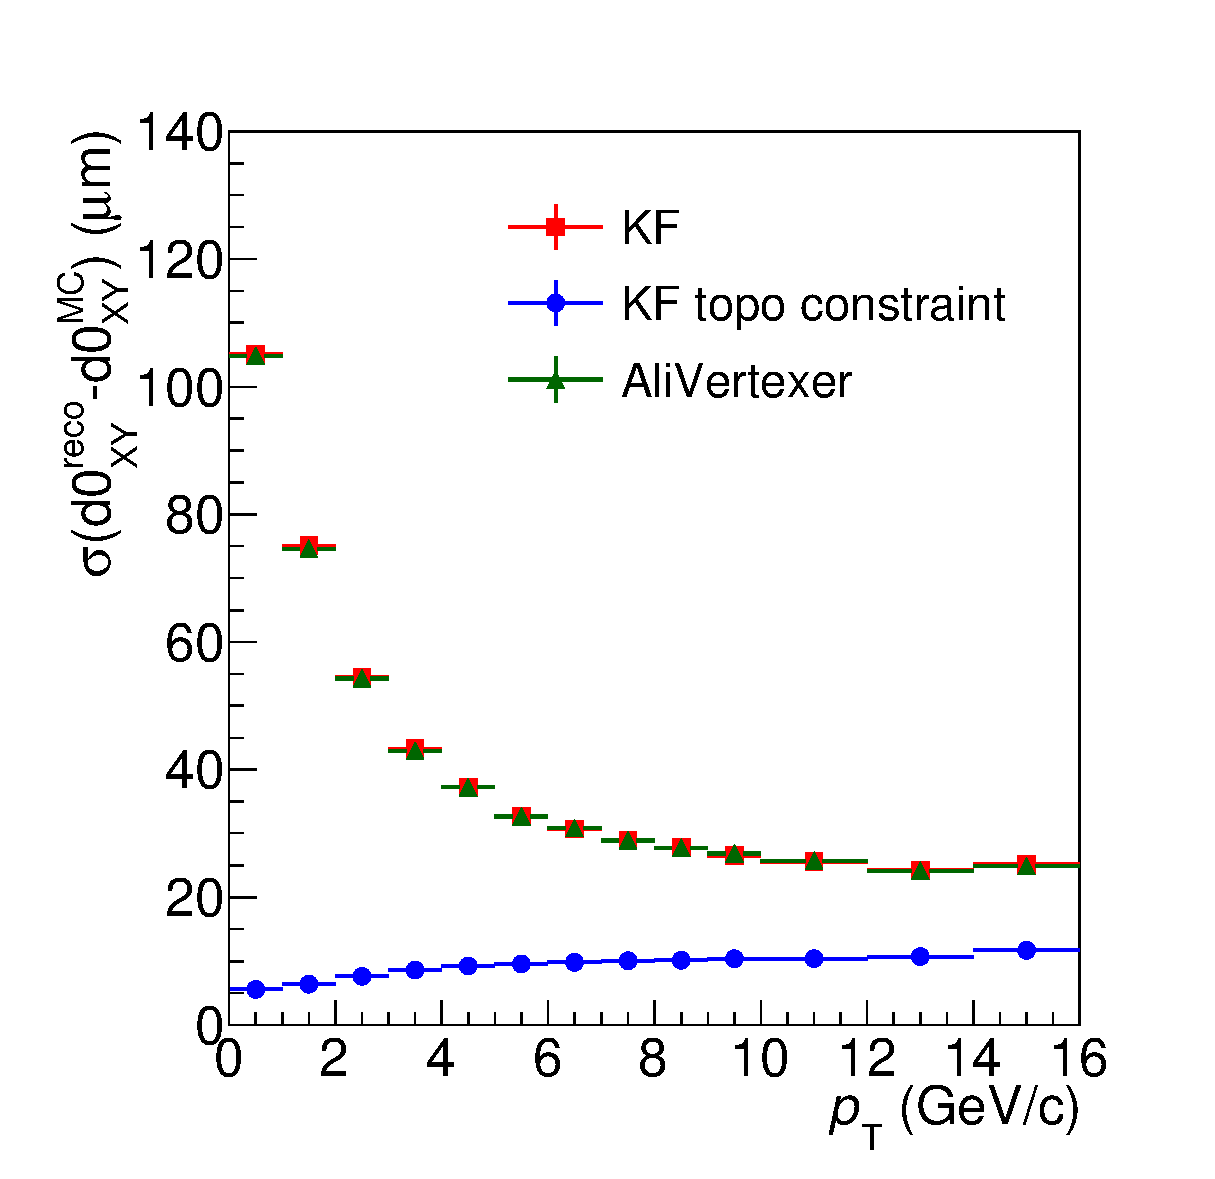
\includegraphics[scale=0.18]{ResImpPar.eps}}

\put(10,245){\captionsetup{labelformat=empty}
\begin{minipage}[t]{0.5\linewidth}
\begin{block}{\centering Filtro di Kalman}
\begin{center}
Algoritmo che permette di stimare un vettore di stato $\pmb{r}$ e la sua matrice delle covarianze $\pmb{C}$ a partire da $n$ misure $\pmb{m}_k$ ($k=1,..,n$) contenenti rumore statistico
\end{center}
\end{block} 
\end{minipage}}

\put(230,245){\captionsetup{labelformat=empty}
\begin{minipage}[t]{0.3\linewidth}
\begin{block}{\centering KFParticle package}
\begin{center}
Pacchetto per la ricostruzione di vertici di decadimento sviluppato per l'esperimento CBM basato sul filtro di Kalman \\$\Downarrow$\\ vettore di stato:\\ $\pmb{r} = (x,y,z,p_x,p_y,p_z,E,s)$
\end{center}
\end{block} 
\end{minipage}}

\put(195,205){
\begin{tikzpicture}[->]
\draw[draw=blue,solid,line width=0.3mm] (0, 0) -- + (0.8,0);
\end{tikzpicture}}

\put(0,160){\captionsetup{labelformat=empty}
\begin{minipage}[t]{0.8\linewidth}
\textcolor{blue}{Vantaggi del KFParticle package}:
\begin{itemize}
\item Valutazione del vettore di stato e della \\matrice di covarianza lungo la traiettoria \\della particella valutata con il filtro di Kalman
\item Possibilità di fissare dei vincoli $\Rightarrow$ \textit{mass constraint, \textcolor{blue}{topological constraint}}
\end{itemize}
\end{minipage}}

\put(0,85){\captionsetup{labelformat=empty}
\begin{minipage}[t]{0.35\linewidth}
Test delle performance eseguito sulla simulazione Monte Carlo selezionando i mesoni D$^+$ \textcolor{blue}{prompt}\\
$\Rightarrow$ risoluzione della variabile $X$:\\
\[Res(\pt) = \sigma(X_{reco}-X_{MC}) (\pt)\]
\end{minipage}}

\end{picture}
\end{frame}

\begin{frame}
\frametitle{Distribuzioni di $\chi^2/ndf$ dopo l'applicazione del \textit{topological constraint}}
\begin{picture}(320,250)

\put(0,235){\captionsetup{labelformat=empty}
\begin{minipage}[t]{1.\linewidth}
I mesoni D$^+$ feed-down  \textcolor{blue}{non} derivano dal vertice primario di interazione dei fasci \\[1mm]
$\Rightarrow$ L'applicazione del \textcolor{blue}{topological constraint} permette di ridurre il contributo di mesoni D$^+$ da B, valutando il \textcolor{blue}{$\chi^2$} della particella ricostruita
\end{minipage}}

\put(35,80){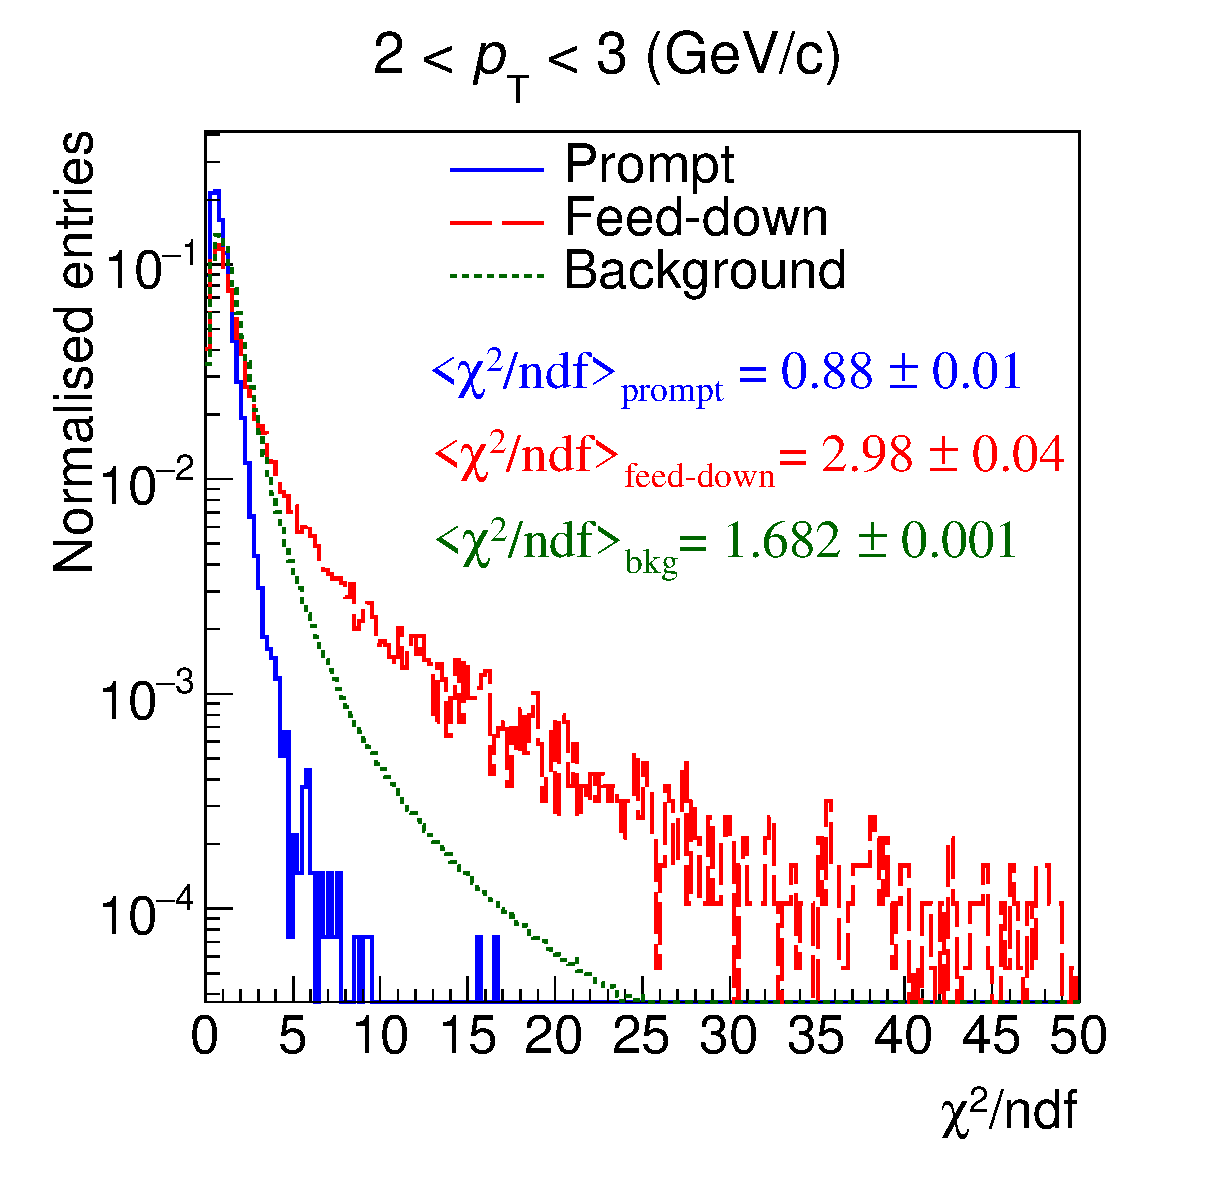
\includegraphics[scale=0.22]{KFchi_Dplus_pT1.eps}}
\put(180,80){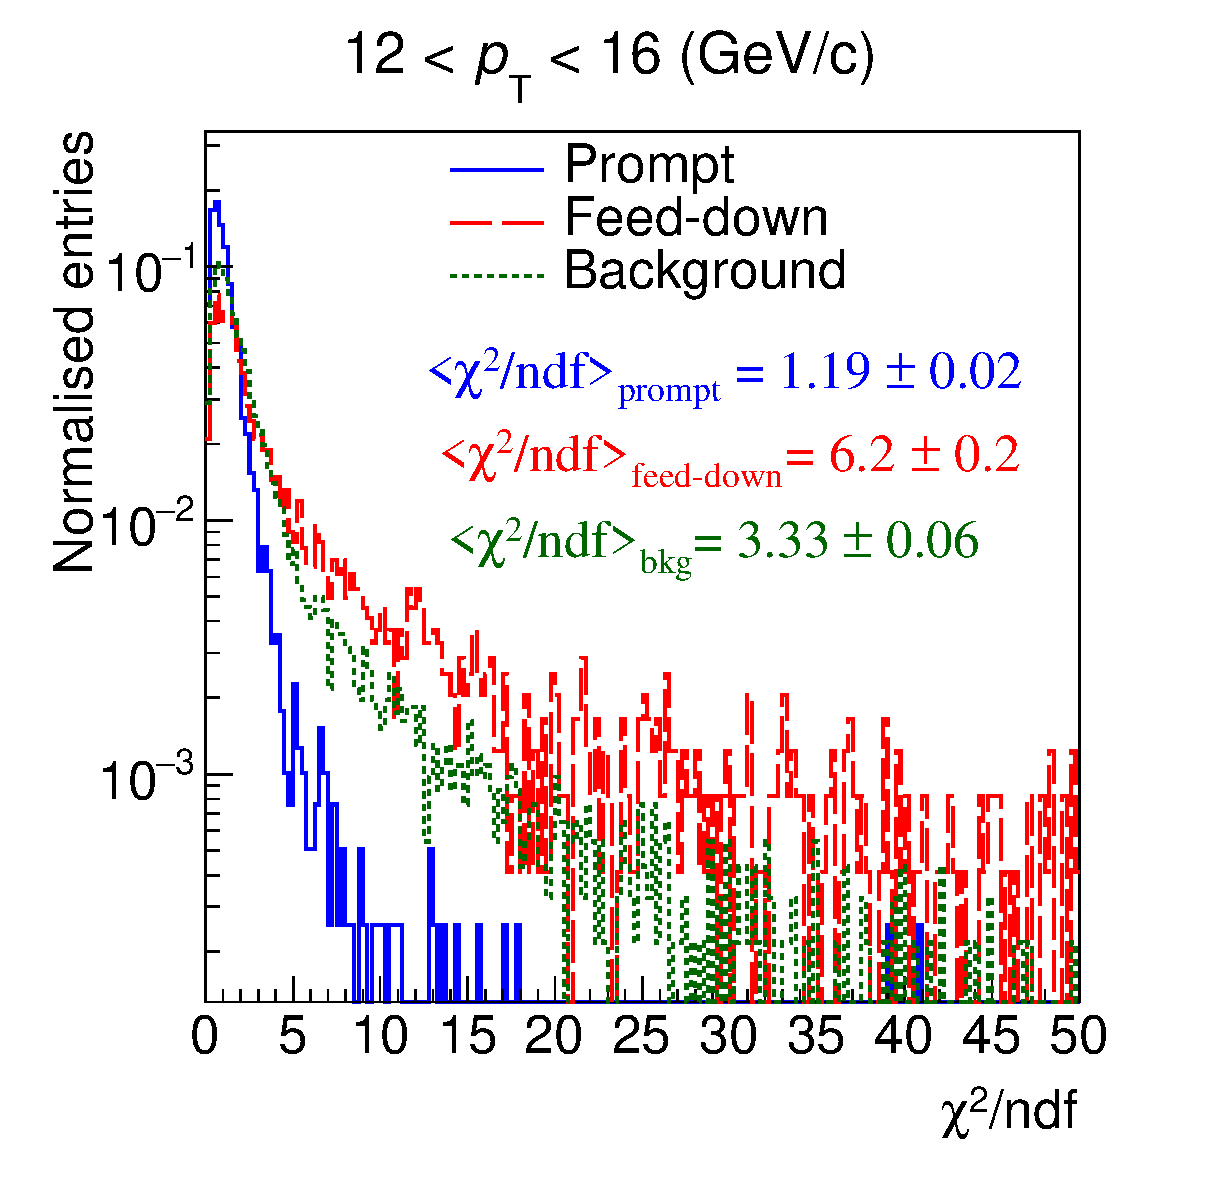
\includegraphics[scale=0.22]{KFchi_Dplus_pT8.eps}}

\put(0,70){\captionsetup{labelformat=empty}
\begin{minipage}[t]{1.\linewidth}
$\Rightarrow$ selezione su $\chi^2/ndf$ delle candidate, oltre alle selezioni sulle quantità topologiche usate nell'analisi standard 
\end{minipage}}

\put(80,35){\captionsetup{labelformat=empty}
\begin{minipage}[t]{0.9\linewidth}
\renewcommand\arraystretch{1.4} 
  \begin{tabular}{c|c|c|c|c}
    $\pt$ (GeV/c) & $[1,2]$ & $[2,8]$ & $[8,16]$ & $[16,24]$ \\
    \hline
    $\chi^2/ndf$ & $<2.5$ & $<3.0$ & $<3.5$ & $<4.0$ \\
    \end{tabular}
\end{minipage}}

\end{picture}
\end{frame}

\begin{frame}
\frametitle{Studio della variazione della selezione su $\chi^2/ndf$}
\begin{picture}(320,250)

\put(10,15){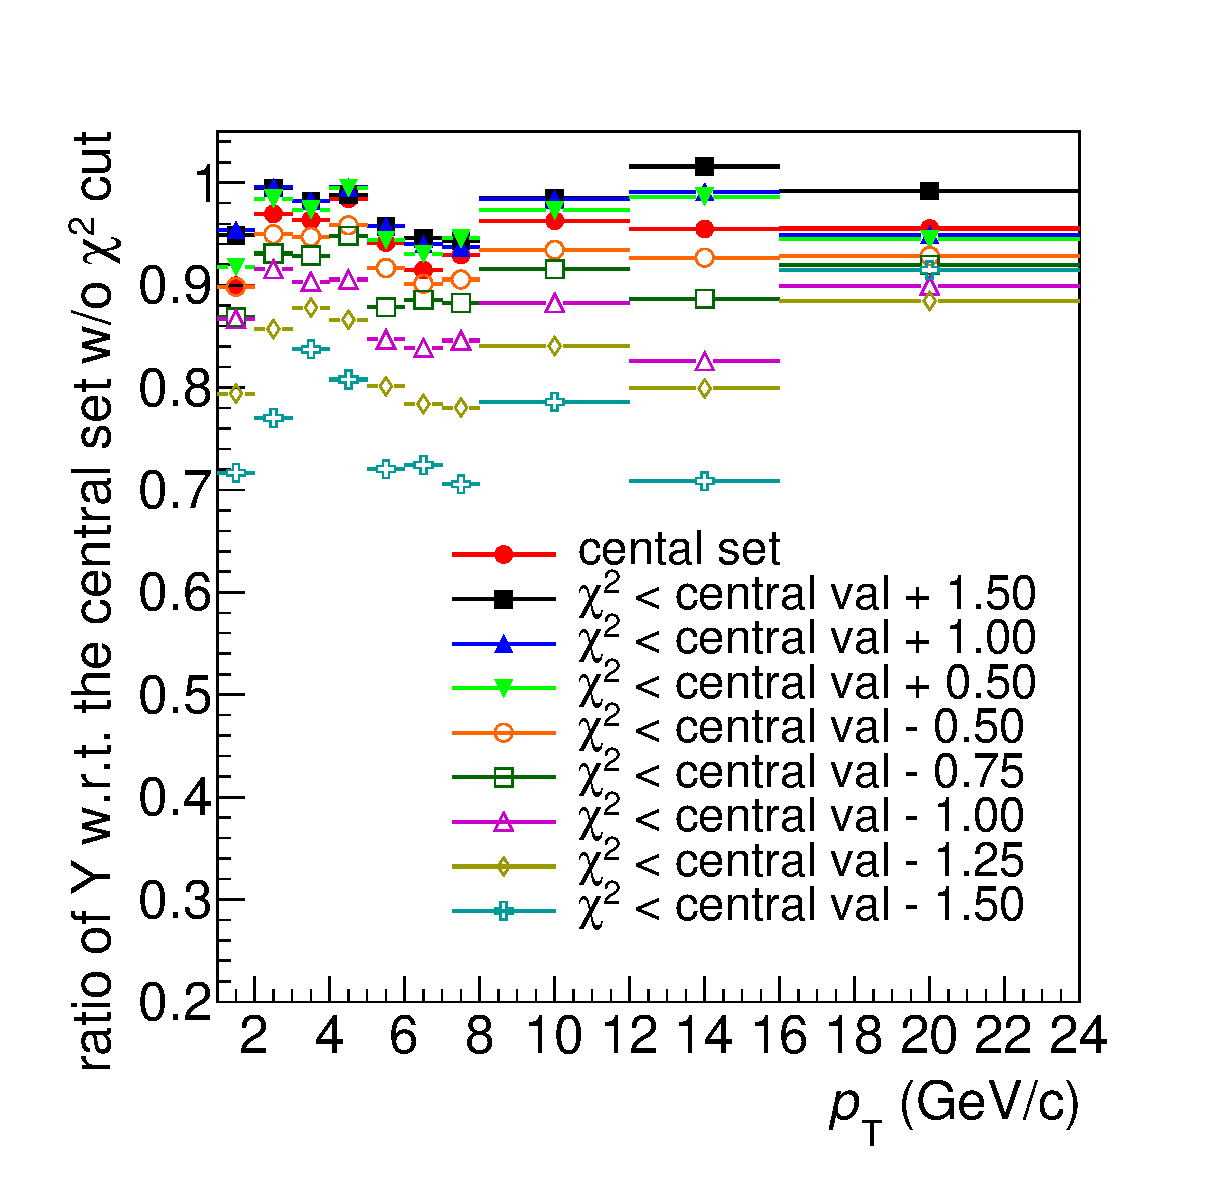
\includegraphics[scale=0.2]{KF_CutVarSyst_ratioraw_chiS.eps}}
\put(130,130){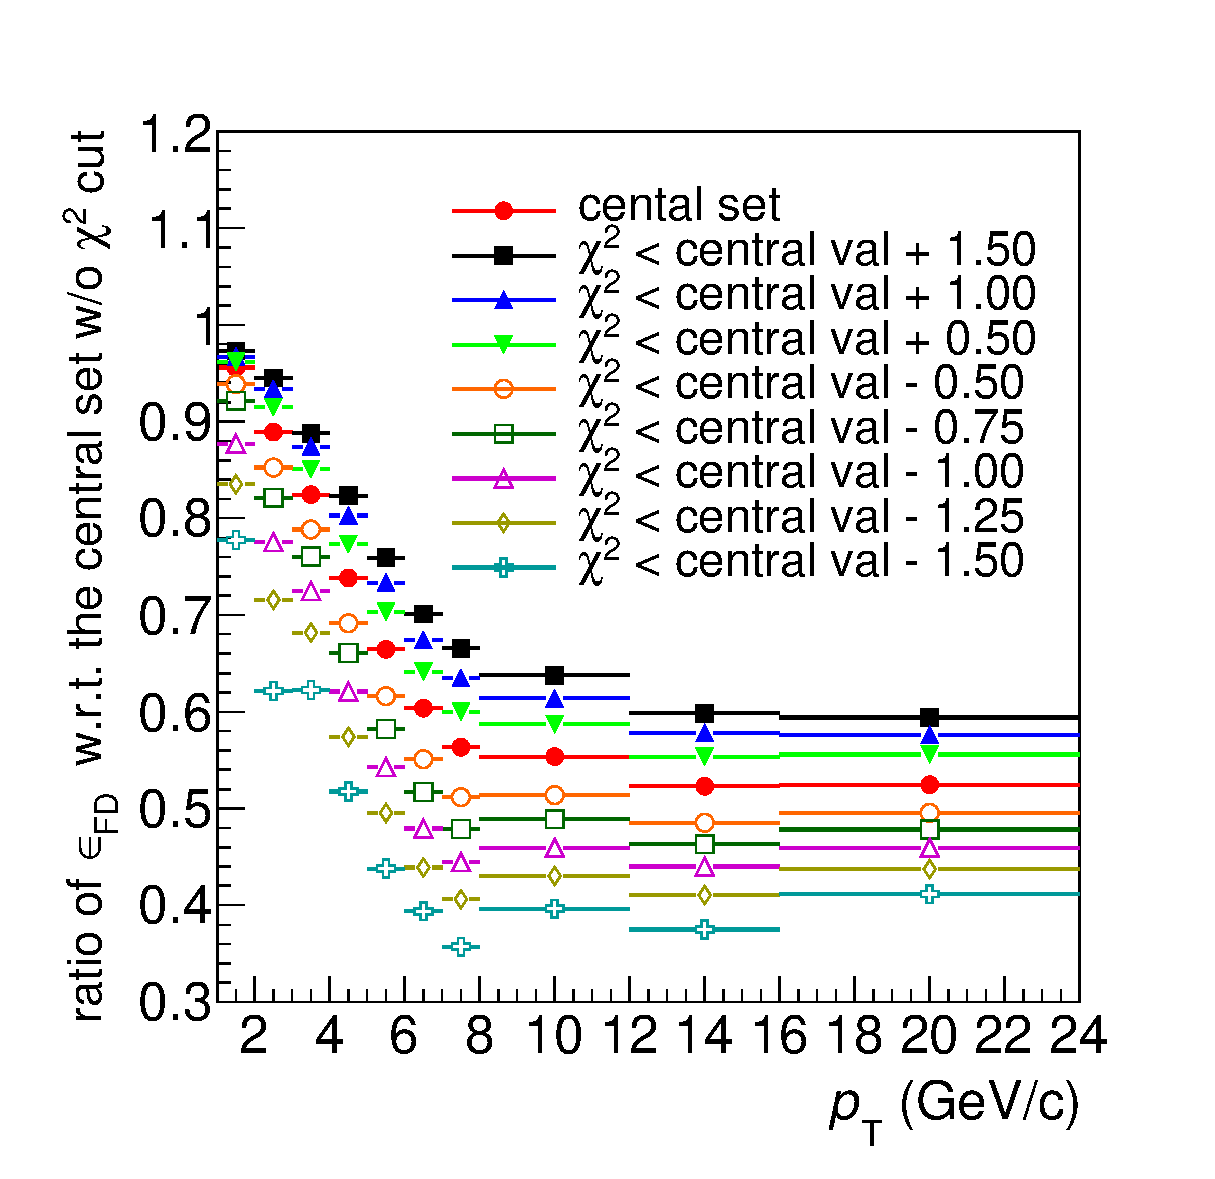
\includegraphics[scale=0.2]{KF_CutVarSyst_ratioeffFD_chiS.eps}}
\put(10,130){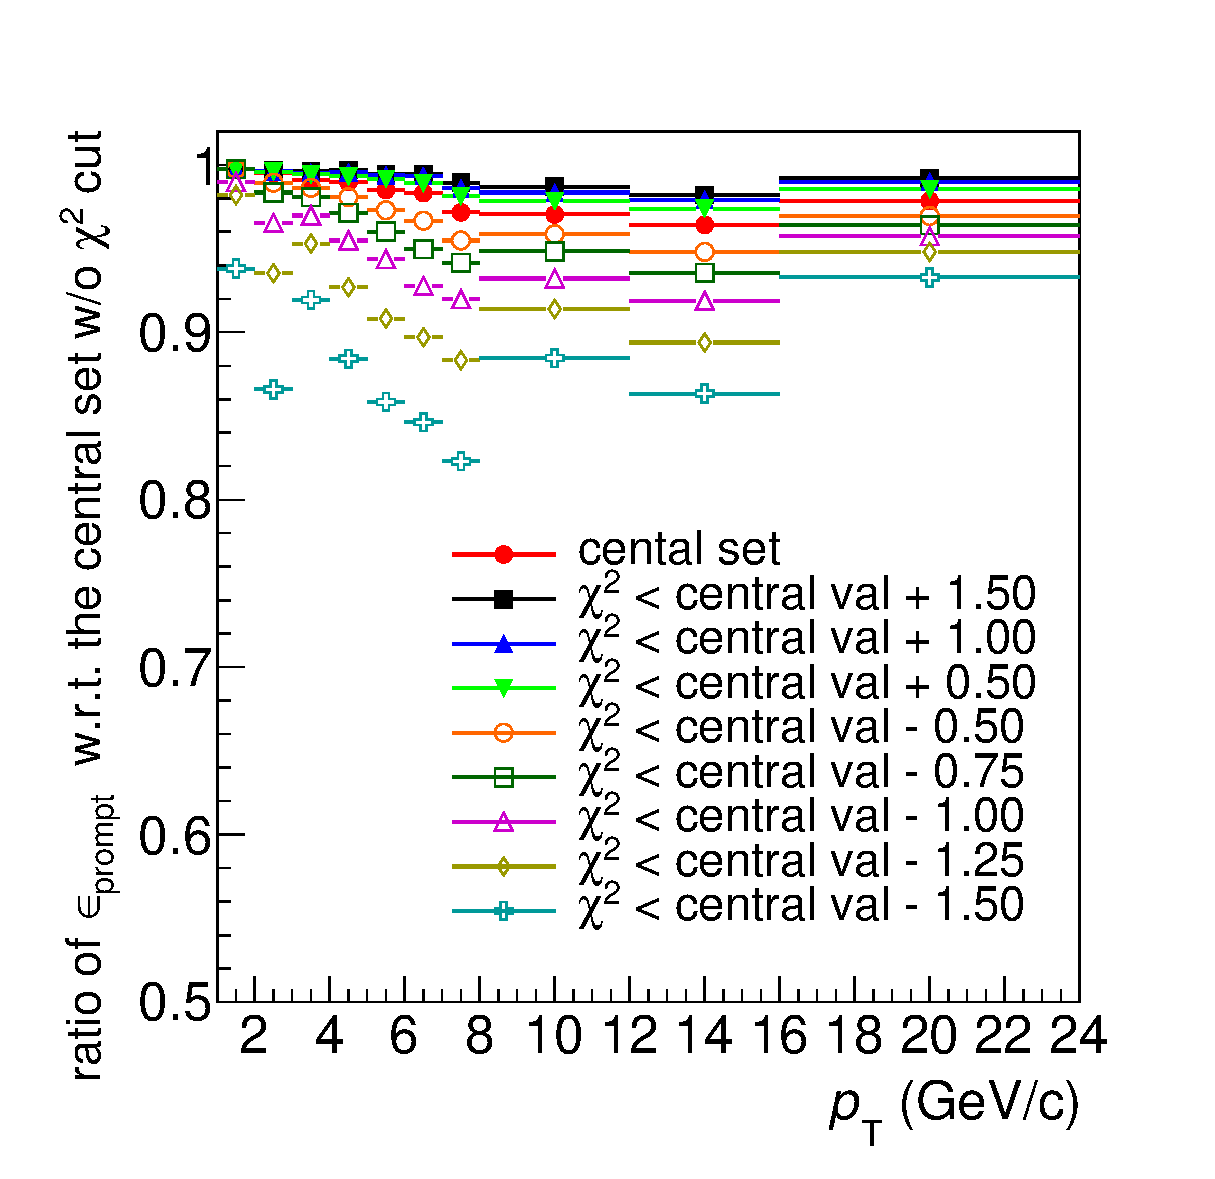
\includegraphics[scale=0.2]{KF_CutVarSyst_ratioeffprompt_chiS.eps}}
\put(130,15){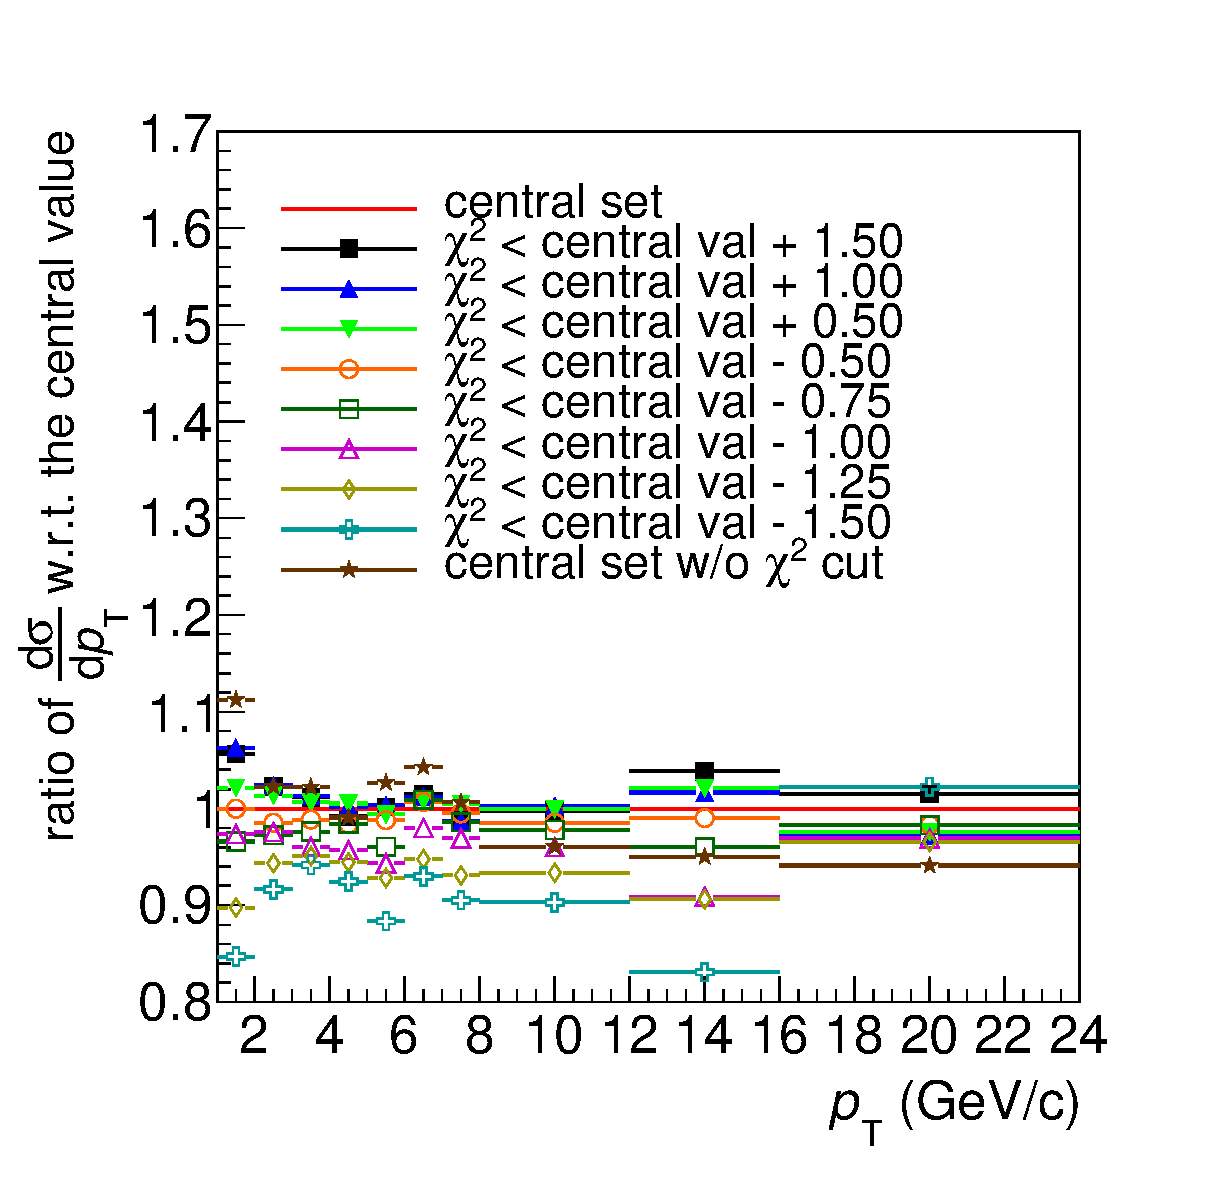
\includegraphics[scale=0.2]{KF_CutVarSyst_ratioonly_chiS.eps}}

\end{picture}
\end{frame}

\begin{frame}
\frametitle{Ricostruzione dei mesoni D$^+$ con il filtro di Kalman - Risultato}
\begin{picture}(320,250)

\put(10,140){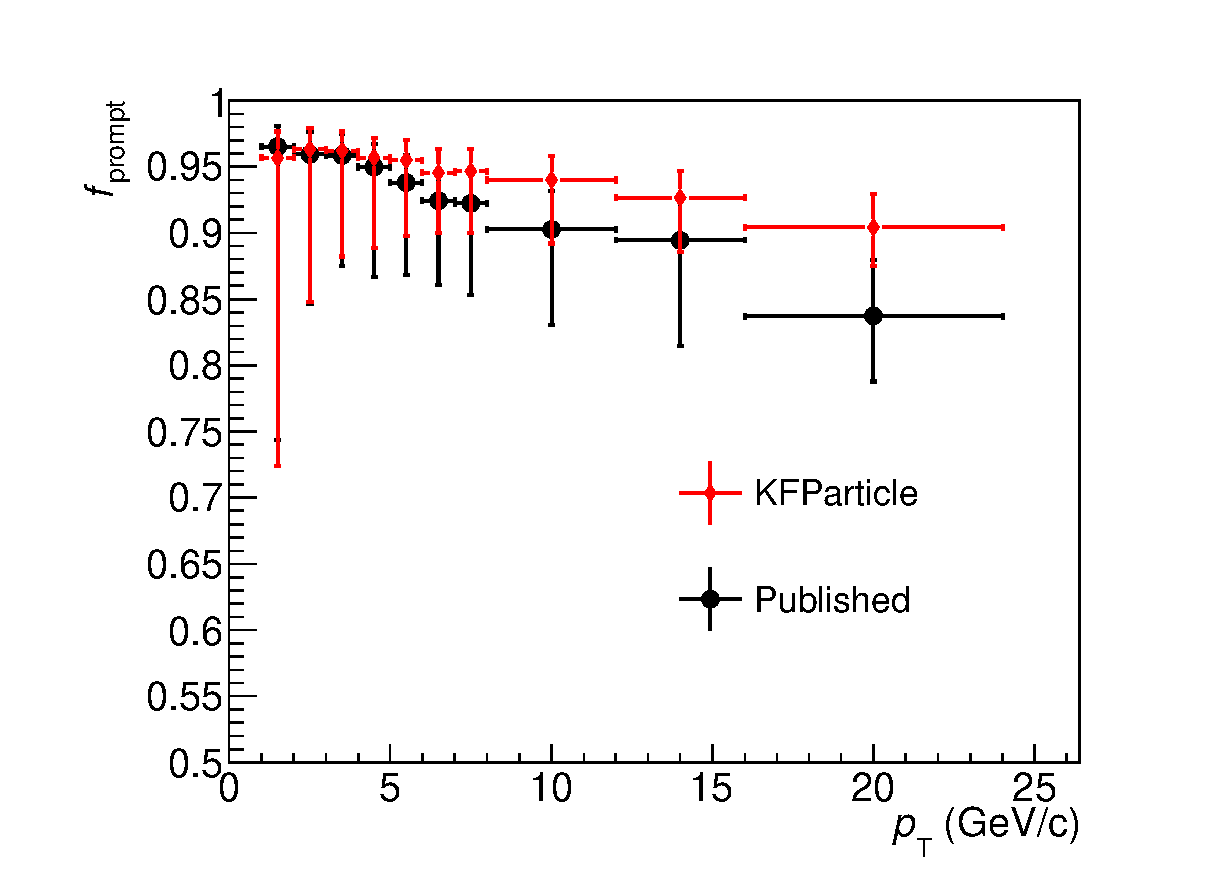
\includegraphics[scale=0.27]{PromptFrac_KF.eps}}
\put(180,80){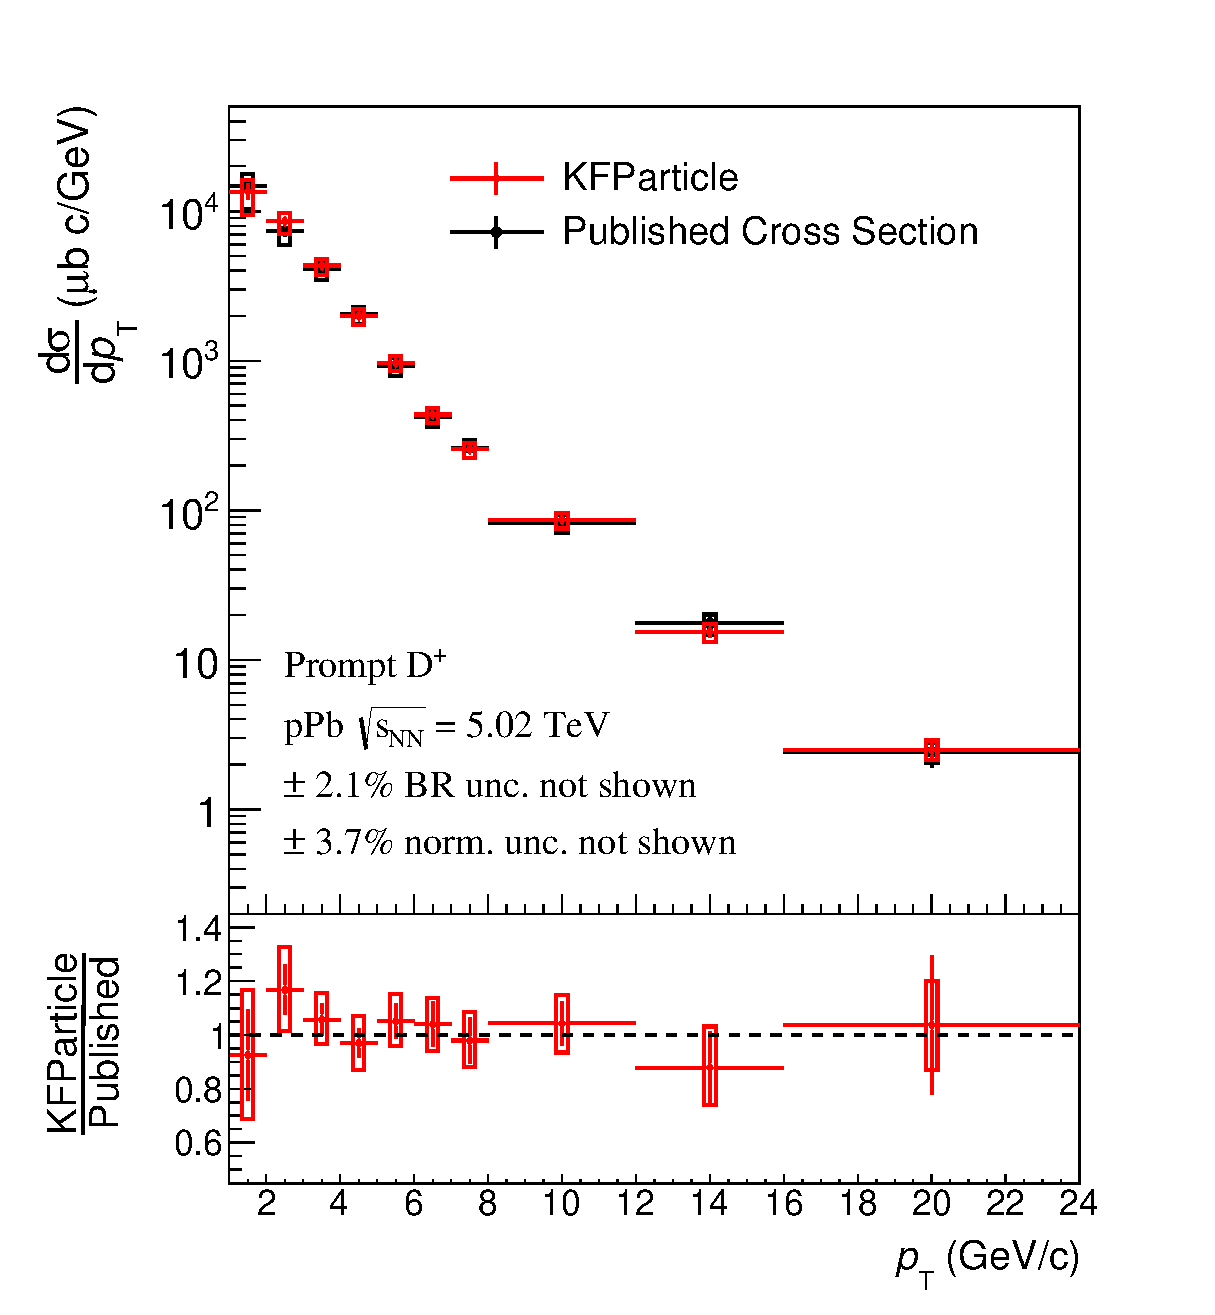
\includegraphics[scale=0.27]{CrossSection_KF.eps}}

\end{picture}
\end{frame}

\begin{frame}
\frametitle{Conclusioni e confronto}
\begin{picture}(320,250)
\put(0,85){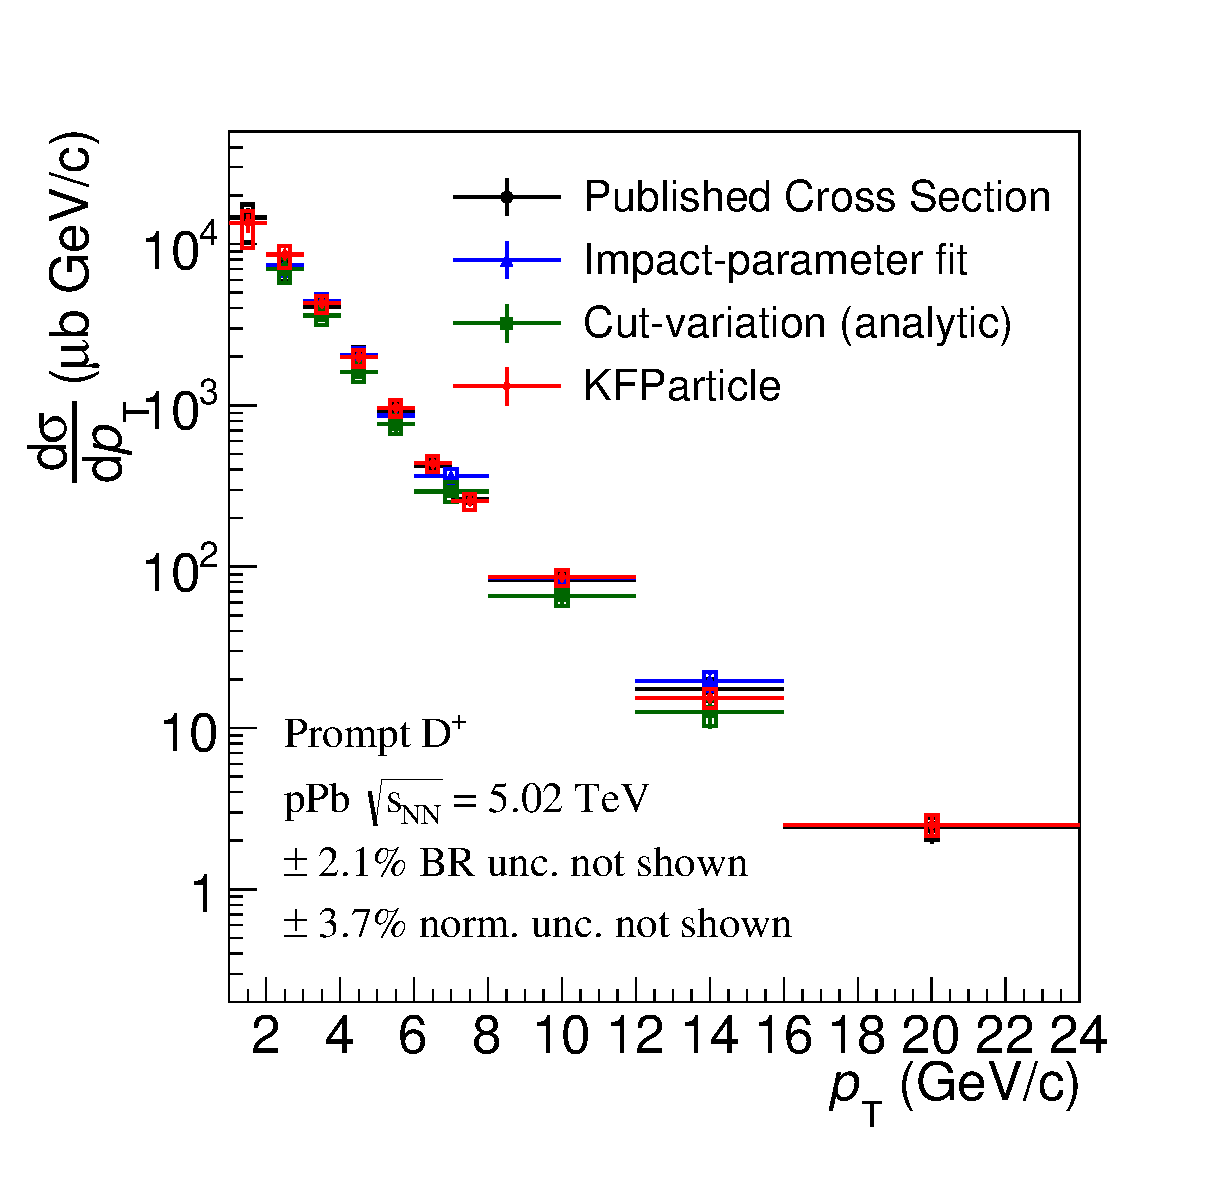
\includegraphics[scale=0.3]{CrossSecComp.eps}}

\end{picture}
\end{frame}

\section{Backup}
\begin{frame}
\frametitle{}
\begin{picture}(320,250)

\put(70,120){
\begin{minipage}[t]{0.55\linewidth}
\begin{center}
\fontsize{1.5cm}{1.75cm}\selectfont{\textcolor{blue}{BACKUP}}
\end{center}
\end{minipage}}

\end{picture}
\end{frame}

\begin{frame}
\frametitle{Confronto dei dati con la predizione di FONLL in collisioni pp}
\begin{picture}(320,250)

\put(0,65){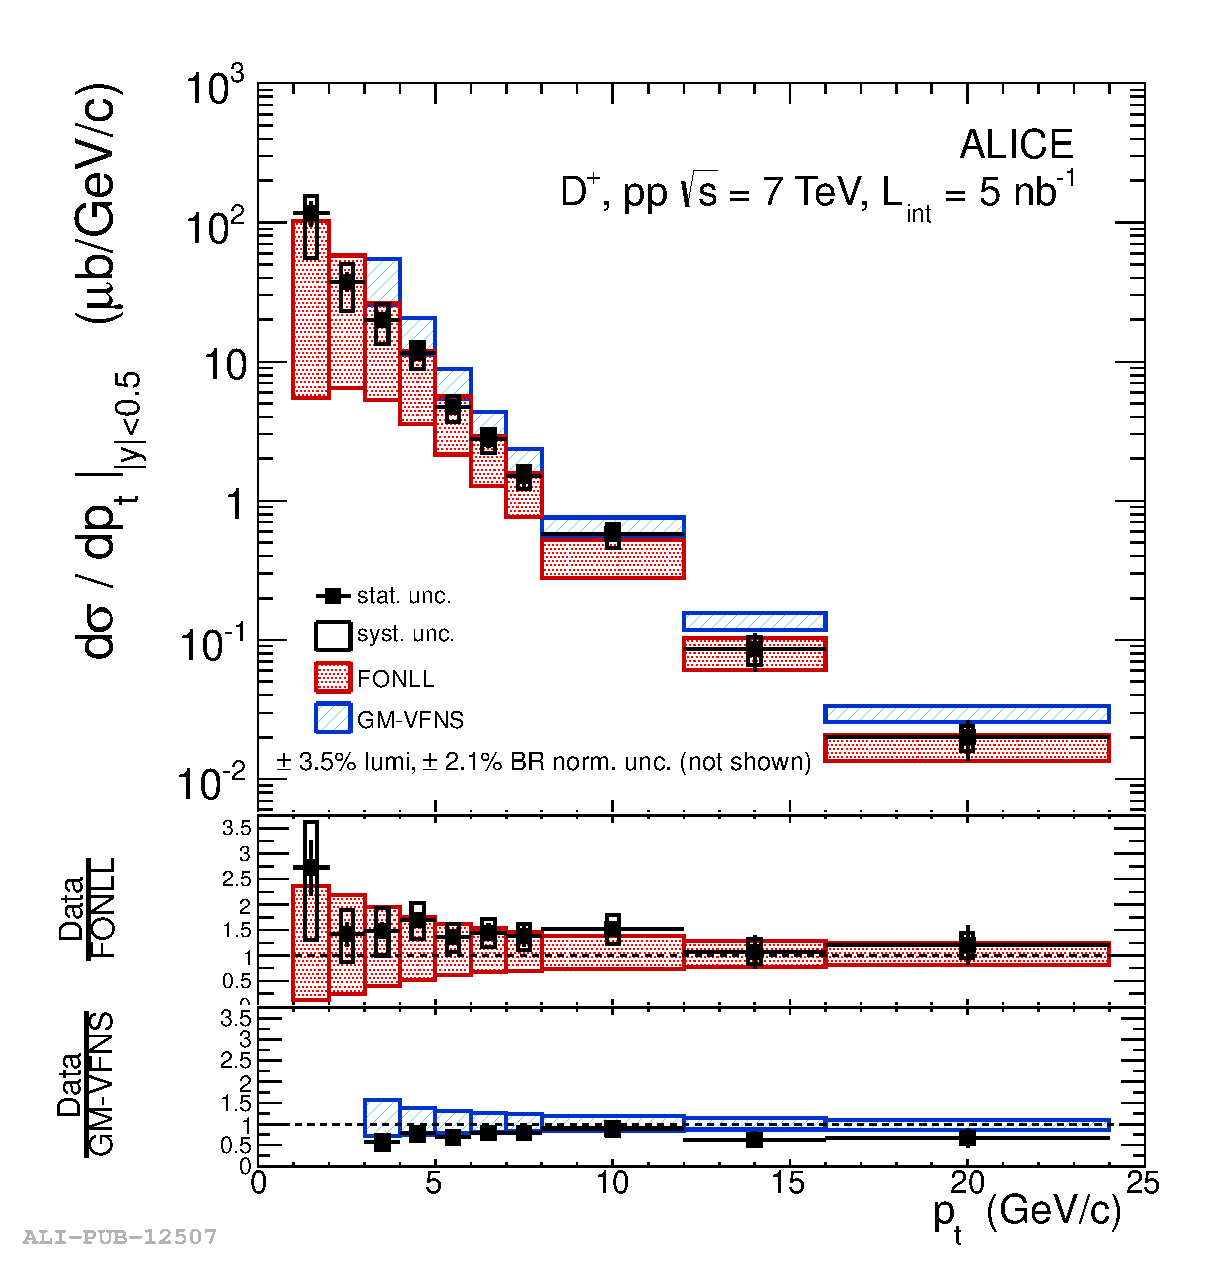
\includegraphics[scale=0.3]{2012-Jun-06-DplusCrossSection_pp7TeV.eps}}
\put(175,65){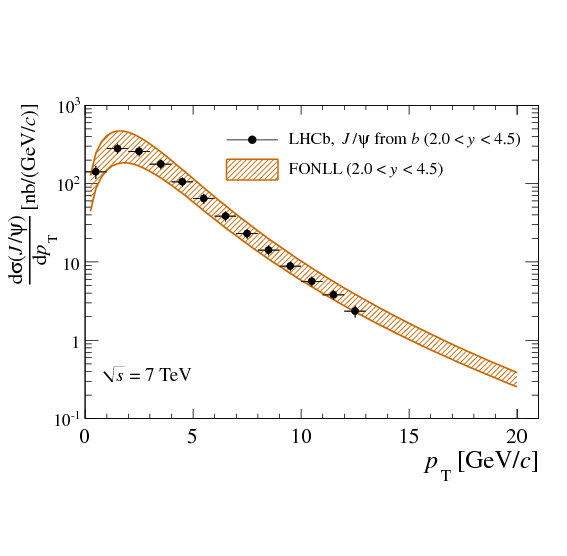
\includegraphics[scale=0.3]{jpsi_nonprompt_LHCb.png}}

\put(10,50){\captionsetup{labelformat=empty}
\begin{minipage}[t]{0.9\linewidth}
\begin{center}
Le sezioni d'urto per adroni contenenti $charm$ e $beauty$ misurate in collisioni pp sono in accordo con la predizione di FONLL \\$\Rightarrow$ nei metodi \textit{theory-driven} la sezione d'urto è calcolata utilizzando FONLL
\end{center}
\end{minipage}}

\end{picture} 
\end{frame}

\end{document}